\documentclass[10pt,b5paper,twoside]{book}

\usepackage[dutch,british]{babel}
\usepackage[nottoc]{tocbibind}
\usepackage{amsmath}
\usepackage{amsfonts}
\usepackage{amssymb}
\usepackage{graphicx}
\usepackage{gensymb}
\usepackage{textcomp}
\usepackage{hyperref}
\usepackage{doi}
\usepackage{xcolor}
\usepackage{nameref}
\usepackage{xspace}
\usepackage{titlesec}
\usepackage{fancyhdr}
\usepackage{wrapfig}
\usepackage{lmodern}
\usepackage[font={scriptsize, sf}, labelfont={sf,scriptsize,bf}]{caption}
\usepackage{apacite}
%\usepackage[Gray,squaren,thinqspace,thinspace]{SIunits}

\hypersetup{colorlinks=true, linkcolor=blue}
\setcounter{tocdepth}{2}

% Do not add extra vertical space
\raggedbottom

% Indent paragraphs
\setlength{\parindent}{1.0cm}

%\bibliographystyle{plain_custom}
\bibliographystyle{apacite_custom}

\renewcommand{\baselinestretch}{1.2}
\setlength{\parskip}{0ex plus 0.3ex minus 0.3ex}
\newcommand{\npar}{\par}
\newcommand{\mbet}{\par \vspace{1.5ex plus 0.02ex minus 0.02ex}}

% Emphasize and insert into index
\newcommand{\concept}[1]{\index{#1}\textbf{#1}\xspace}


\hypersetup{
    pdfauthor = {Ivar Clemens},
    %pdftitle = {Choosing our words},
    %pdfsubject = {Language production},
    %pdfkeywords = {language production; }
}

\newcommand{\textapprox}{\raisebox{0.5ex}{\texttildelow}}
\newcommand{\SBT}[1]{$\text{SBT}_\text{#1}$}

%% For the Chapter title, etc.
\newcommand{\bigrule}{\titlerule[0.5mm]}
\titleformat{\chapter}[display]
{\normalfont\filleft\bfseries\itshape}
{%
 \vskip-3em
\titlerule[1pt]%
\vspace{1pt}%
\titlerule
\vspace{1pc}%
\Large\MakeUppercase{\chaptertitlename} \thechapter}
{1pc}
{\titlerule
\vspace{1pc}%
\Huge}


%%%%%%%%%%%
% Document
%%%%%%%%%%%


\begin{document}

%%%%%%%%%%%%%%%
% Front matter

\frontmatter
\begin{titlepage}

\fontsize{12pt}{14pt}\selectfont

\qquad

\fontsize{17.28pt}{21pt}\selectfont

\noindent \concept{The title comes here}
\fontsize{15.28pt}{20pt}\selectfont
 \npar \noindent Subtitle comes here

\fontsize{12pt}{14pt}\selectfont

\vspace{1cm}

\noindent \concept{Ivar Clemens}

\vspace{3cm}

\end{titlepage}

\thispagestyle{empty}

%%%%%%%%%%%%%%%%%
% COPYRIGHT PAGE

\clearpage
\pagestyle{empty}
	
\null
\vfill
\noindent ISBN: rep-la-cethi-s!-!
\npar
%\noindent Illustration: Camila Tamie Piai
%\npar
\noindent Printed by Ipskamp Drukkers, Nijmegen, The Netherlands
\npar
\noindent \copyright 2014 Ivar Clemens


%%%%%%%%%%%%%%%%%%%%%%%
% MANDATORY TITLE PAGE

\begin{titlepage}

\fontsize{12pt}{14pt}\selectfont
\vspace*{\fill}
\begin{center}

\fontsize{17.28pt}{21pt}\selectfont

{\textsc{REPLACE WITH TITLE}}
 \npar REPLACE WITH SUBTITLE

\fontseries{m}
\fontsize{12pt}{14pt}\selectfont

\vspace{1cm}
Proefschrift
\vspace{1cm}
\npar
ter verkrijging van de graad van doctor
\npar
aan de Radboud Universiteit Nijmegen
\npar
op gezag van de rector magnificus prof. mr. S.C.J.J. Kortmann, 
\npar
volgens besluit van het college van decanen
\npar
in het openbaar te verdedigen op [dow] [dow] [month] [year]
\npar
om [hour].[min] precies
\npar
\vspace{1cm}
door
\npar
\vspace{1cm}
\concept{Ivar Clemens}
\npar
geboren op 2 juni 1984
\npar
te Boxtel, Nederland

\vspace{2.8cm}

\fontsize{17.28pt}{21pt}\selectfont

\end{center}
\end{titlepage}

\thispagestyle{empty}


%%%%%%%%%%%%%%%%%%%%%
% BACK OF TITLE PAGE

\clearpage
\pagestyle{empty}
	
\noindent \concept{Promotoren:}
\noindent \npar Prof. dr. W.P. Medendorp
\npar
\vspace{0.5cm}
\noindent \concept{Manuscriptcommissie:}
\noindent \npar Prof. dr. F. Surname


% Table of contents
\newpage
\renewcommand{\baselinestretch}{1.08}
\small\normalsize
\tableofcontents
\renewcommand{\baselinestretch}{1.2}
\small\normalsize


%%%%%%%%%%%%%%
% Actual text

\mainmatter
\selectlanguage{british}
\chapter{General introduction}
\newpage
...

\documentclass[10pt,b5paper,twoside]{book}


%
% Common packages and custom commands used by the main .tex files.
%

\usepackage[dutch,british]{babel}
\usepackage[nottoc]{tocbibind}
\usepackage{amsmath}
\usepackage{amsfonts}
\usepackage{amssymb}
\usepackage{graphicx}
\usepackage{gensymb}
\usepackage{textcomp}
\usepackage{hyperref}
\usepackage{doi}
\usepackage{xcolor}
\usepackage{nameref}
\usepackage{xspace}
\usepackage{titlesec}
\usepackage{floatrow}
\usepackage{longtable}
\usepackage{siunitx}
\usepackage[outercaption]{sidecap}
%\usepackage{fancyhdr}
\usepackage{wrapfig}
\usepackage{lmodern}
\usepackage[font={scriptsize, sf}, labelfont={sf,scriptsize,bf}]{caption}
\usepackage{src/apacite_custom}
\usepackage{src/thesis}

\pagestyle{plain}

\floatsetup[table]{font={scriptsize, sf}}

\hypersetup{colorlinks=true, linkcolor=blue, citecolor=blue}
\setcounter{tocdepth}{2}

% Do not add extra vertical space
\raggedbottom

% Indent paragraphs
\setlength{\parindent}{1.0cm}

\bibliographystyle{apacite_custom}

\renewcommand{\baselinestretch}{1.2}
\setlength{\parskip}{0ex plus 0.3ex minus 0.3ex}

\newcommand{\about}{$\approx$}

%% For the Chapter title, etc.
\newcommand{\bigrule}{\titlerule[0.5mm]}
\titleformat{\chapter}[display]
{\normalfont\filleft\bfseries\itshape}
{%
 \vskip-3em
\titlerule[1pt]%
\vspace{1pt}%
\titlerule
\vspace{1pc}%
\Large\MakeUppercase{\chaptertitlename} \thechapter}
{1pc}
{\titlerule
\vspace{1pc}%
\thispagestyle{empty}
\Huge}


\hypersetup{
    pdfauthor = {Ivar Clemens, Maaike de Vrijer, Luc Selen, Jan van Gisbergen, and Pieter Medendorp},
    pdftitle = {Multisensory processing in spatial orientation:\\An inverse probabilistic approach},
    %pdfsubject = {Language production},
    %pdfkeywords = {language production; }
}

\begin{document}

\selectlanguage{british}

\chapter{Multisensory processing in spatial orientation:\\An inverse probabilistic approach}
\chaptermark{}
\label{p1}

\newpage

\small {\bf Abstract} Most evidence that the brain uses Bayesian inference to integrate noisy sensory signals optimally has been obtained by showing that the noise levels in each modality separately can predict performance in combined conditions. Such a forward approach is difficult to implement when the various signals cannot be measured in isolation, as in spatial orientation, which involves the processing of visual, somatosensory, and vestibular cues. Instead, we applied an inverse probabilistic approach, based on optimal observer theory. Our goal was to investigate whether the perceptual differences found when probing two different states -- body-in-space and head-in-space orientation -- can be reconciled by a shared scheme using all available sensory signals. Using a psychometric approach, seven human subjects were tested on two orientation estimates at tilts \textless 120\textdegree: perception of body tilt [subjective body tilt (SBT)] and perception of visual vertical [subjective visual vertical (SVV)]. In all subjects, the SBT was more accurate than the SVV, which showed substantial systematic errors for tilt angles beyond 60\textdegree. Variability increased with tilt angle in both tasks, but was consistently lower in the SVV. The sensory integration model fitted both datasets very nicely. A further experiment, in which supine subjects judged their head orientation relative to the body, independently confirmed the predicted head-on-body noise by the model. Model predictions based on the derived noise properties from the various modalities were also consistent with previously published deficits in vestibular and somatosensory patients. We conclude that Bayesian computations can account for the typical differences in spatial orientation judgments associated with different task requirements.

\vfill

\noindent\underline{ \hspace{4cm} }

\noindent This chapter has been published as \newline
\noindent {\bf Clemens, I.A.H.}, De Vrijer, M., Selen, L.P.J., Van Gisbergen, J.A.M. and Medendorp, W.P. \citeyear{clemens2011}. Multisensory processing in spatial orientation: An inverse probabilistic approach. \emph{Journal of Neuroscience}, 31(14): 5365-5377. \newline
%\noindent Authors Clemens and De Vrijer contributed equally to this work.

\newpage

%%%%%%%%%
% Intro %
%%%%%%%%%

\section{Introduction}

To infer the current state of the body in space, the brain must rely on noisy sensory inputs. Thus, a degree of uncertainty in the reconstructed physical state is unavoidable. However, according to the rules of Bayesian inference, perceptual uncertainty can be reduced by combining overlapping information from different sensory modalities, weighting each signal in proportion to its reliability \cite{knill2004,kording2004,angelaki2008}. For example, psychophysical studies have shown that human observers behave optimally when integrating visual--proprioceptive \cite{vanbeers1999}, visual--haptic \cite{ernst2002}, or visual--auditory \cite{alais2004} cues. In these studies, the approach was to estimate noise levels of the two sensory modalities in separate unimodal experiments that were then used to predict performance in the bimodal case. Unfortunately, such a forward approach is difficult to implement when the involved sensory modalities cannot be studied in isolation, as in spatial orientation, which involves visual, somatosensory, and vestibular cues. Here the visual contribution can be eliminated easily, but to test whether somatosensory and vestibular cues are combined optimally, one cannot simply ``switch off'' one system to assess the noise level of the other.

Instead, we took optimality as a starting point and implemented an inverse probabilistic approach to deduce noise levels of the various individual sensors. We probed two spatial orientation estimates---body-in-space and head-in-space orientation--- which, according to optimal theory, will use all available sensory signals that can be obtained by various reference frame transformations. This transformation and integration scheme, shown in \figref{p1:fig1}, involves at least three sensory systems: (1) head sensors, supplying information about the orientation of the head with respect to gravity (vestibular system); (2) body sensors, providing an estimate of the orientation of the body in space (``somatic graviceptors'') \cite{mittelstaedt1997}; and (3) neck sensors, providing an estimate of the angle between head and body (neck proprioceptors).

\begin{figure}
    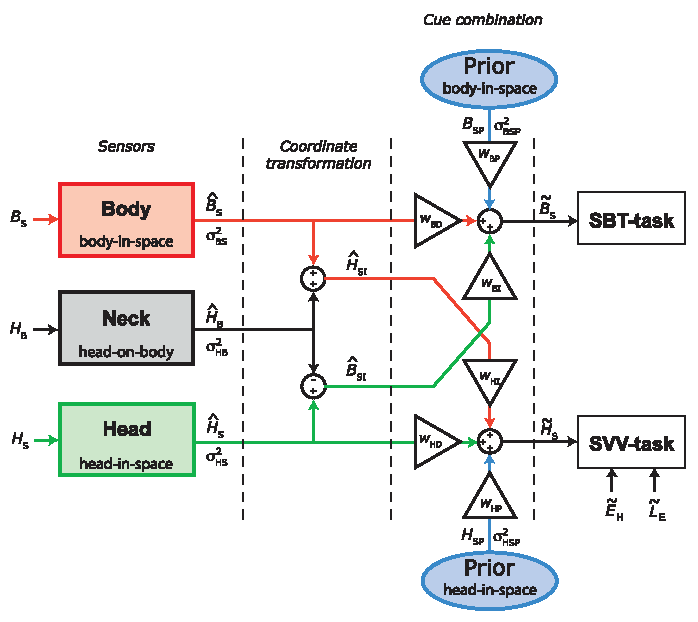
\includegraphics[width=0.75\textwidth]{src/paper1/figure1.pdf}

    \caption{Schematic representation of the sensory integration model. Sensory signals, denoted by a hat symbol (\textasciicircum), are assumed to be calibrated accurately, but contaminated by Gaussian noise. Optimal estimates are denoted by a tilde (\textasciitilde). Body sensors, neck sensors, and otoliths provide information about orientation of body in space ($B_S$), head on body ($H_B$), and head in space ($H_S$), respectively. Neck signal ($\hat{H}_B$) is used for a reference frame transformation of otolith information into a body-in-space signal ($\hat{H}_S - \hat{H}_B = \hat{B}_{SI}$), and for a transformation of body-tilt information into a head-in-space signal ($\hat{B}_S + \hat{H}_B = \hat{H}_{SI}$). For an optimal estimate of body-in-space orientation, $\tilde{B}_S$ (SBT task), the model combines the body-sensor signal ($\hat{B}_S$, red pathway) with a reference-frame-transformed otolith signal ($\hat{B}_{SI}$, green pathway). Relative contributions of the two pathways ($w_{BD}$ and $w_{BI}$) depend on their relative precision (\eqnref{p1:eqn2}). The scheme shows a symmetrical arrangement with two priors, but there is ample reason to believe that their effects are not identical. The simplest explanation of current and previous SBT data (see \nameref{p1:sec:methods}, \nameref{p1:sec:sbt_computation}) indicates that the associated prior in this task is uniform, which implies that $w_{BP}$ can be ignored. In the SVV task, an optimal estimate of head-in-space ($\tilde{H}_S$) is obtained by integration of otolith information ($\hat{H}_S$, green pathway), reference-frame-transformed information from body sensors ($\hat{H}_{SI}$, red pathway), and a significant contribution from prior information ($H_{SP}$, blue pathway). Relative weights are denoted by $w_{HD}$, $w_{HI}$, and $w_{HP}$, respectively. Estimate of line-in-space orientation is obtained by combining $\tilde{H}_S$ and estimates of eye-in-head ($\tilde{E}_H$) and line-on-eye ($\tilde{L}_E$) orientation. Noise variance in body sensors ($\sigma^2_{BS}$), neck sensors ($\sigma^2_{HB}$), otoliths ($\sigma^2_{HS}$), and width of prior ($\sigma^2_{HSP}$) defines their relative weights (see \nameref{p1:sec:methods}). Otolith noise may depend on tilt angle (\eqnref{p1:eqn11}). Note that the process of sensory integration, denoted here by summation of weighted sensory signals, is equivalent to multiplication of the underlying probability distributions (\eqnref[ and ]{p1:eqn2,p1:eqn6} and \nameref{p1:sec:appendix}).}
    \label{p1:fig1}
\end{figure}

In this scheme, an estimate of body orientation in space can be obtained directly from the body sensors, but also indirectly from the head-sensor signal, by subtracting the neck signal. Likewise, the estimate of head-in-space orientation can be obtained from the head sensors, but also through an indirect pathway, by combining the body-sensor signal with neck information. Importantly, as the two state estimates require different transformations, Bayesian theory predicts that the relative contribution of the sensory signals will differ as well \cite{mcguire2009}. Apart from the crucial role of sensory information, the scheme allows for the possibility that the estimates of the two orientation states can be further influenced by prior beliefs about sensory states.

Here, we used two psychophysical tasks -- subjective body tilt (SBT) and subjective visual vertical (SVV) to quantify the two orientation estimates in a group of healthy subjects. Using an inverse probabilistic approach, we obtained stable solutions for the noise properties of the involved sensor systems. Independent measurements of neck noise confirmed the levels predicted by the model. Forward model predictions based on these noise properties were consistent with previously published deficits of bilateral vestibular and paraplegic patients, which would be difficult to explain otherwise. Our results suggest that Bayesian integration of multisensory information explains the major task-dependent features in spatial orientation perception.


%%%%%%%%%%%
% Methods %
%%%%%%%%%%%

\section{Materials and Methods}
\label{p1:sec:methods}

\subsection{Subjects}

Seven subjects (6 male, 1 female) provided written informed consent to participate in the experiments. Ages ranged from 23 to 65 years. Subjects were free of any known vestibular or other neurological disorder and had normal or corrected-to-normal visual acuity. All subjects took part in SBT and SVV experiments (see below, \nameref{p1:sec:experiments}) and returned to the laboratory for an independent measurement of neck proprioception. Before each experiment started, subjects received careful instructions and performed a few practice runs to get used to the task. Participants never received any feedback about their performance, not even in the training trials. Each subject participated in 20 experimental sessions of {\textapprox}45 min each, yielding {\textgreater}15h recording time per participant.

\subsection{Setup}

Body tilt was controlled by a computer-controlled vestibular chair, which was configured to allow subject rotation in the roll axis. A digital position encoder measured roll position with an angular resolution of \siang{0.04}. The subject's body was tightly fixated using a five-point seat belt and adjustable shoulder and hip supports. Velcro straps restrained both legs and feet, and a padded helmet firmly fixated the head in a natural upright position for looking straight ahead. Subject-specific seat adjustments ensured that the naso-occipital axis, midway between the eyes, coincided with the roll axis of the chair. Experiments took place in complete darkness.

\subsection{Experiments}
\label{p1:sec:experiments}

\subsubsection{SBT}
\label{p1:sec:methods_sbt}

The SBT experiment served to obtain a psychometric measure of each subject's accuracy and precision of body-tilt perception at five body-tilt angles: upright (\siang{0}, \SBT{0} task) and \siang{45} and \siang{90} right side and left side down (\SBT{\textpm45} task and \SBT{\textpm90} task). Negative angles indicated left side down. We applied the method of constant stimuli, using a set of 10 equidistant body-tilt angles, centred on tentative estimates of the subject's \siang{0} (SBT0), \siang{45} (\SBT{45}), \siang{-45} (\SBT{-45}), \siang{90} (\SBT{90}), and \siang{-90} (SBT-90) body-tilt percept. The latter were determined in a few pilot trials that also served to familiarise the subject with the task, without providing a reference of the five respective orientations to be tested. Relative to the test angle, we used test angle intervals of \siang{3}, \siang{4}, and \siang{4} in the \SBT{0}, \SBT{\textpm45}, and \SBT{\textpm90} tasks, respectively. Body-tilt angles were tested 14 times in random order, yielding 140 responses for each psychometric curve.

To perform the psychophysical SBT experiments, two methodological problems had to be solved. The first relates to the number of experimental sessions that we could reasonably ask subjects to perform. We realised that returning the subject to upright for reorientation after each trial would require too large a number of experimental sessions. Our overriding concern was that starting each trial from upright would confound the \SBT{0} task in the sense that subjects could then simply notice the change in chair position. To prevent this, we always inserted a detour rotation before moving the subject to the test angle in a given trial. The detour, always to a tilt position clearly outside the psychometric test range, served to reset the subject's memory of the previous tilt position. These detour angles were chosen randomly from a range at \siang{30-40} clockwise (CW) and counterclockwise (CCW) from the presumed threshold. As an illustration, \figref{p1:fig2} shows how the subject was moved from one trial to the next in the course of an \SBT{90} experiment. Detour angles preceding each test angle were taken from the CW and the CCW detour range in equal proportions. An analysis of trial history effects indicated that detour angles did not affect the judgment in the subsequent trial ($p > 0.05$).

\begin{figure}
%\begin{wrapfigure}{l}[5pt]{0.5\textwidth}
    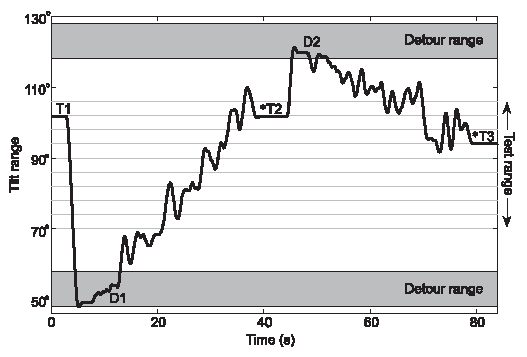
\includegraphics[width=0.75\textwidth]{src/paper1/figure2.pdf}

    \caption{Tilt paradigm in \SBT{90} task. T1, T2, T3, Test angles at which the subject was prompted with a beep signal (*) to indicate whether body orientation was CW or CCW from the instructed reference orientation (i.e., \siang{90} in this example). D1, D2, Detour angles randomly drawn from detour range (\siang{30-40} CW and CCW from centre of test range). Rotations from detour (D) to test (T) angle were performed in a noisy fashion (see \nameref{p1:sec:methods}, \nameref{p1:sec:methods_sbt}).}
    \label{p1:fig2}
%\end{wrapfigure}
\end{figure}

Each experimental run started in upright position with the room lights on. After the lights were turned off, subjects were first rotated at a constant angular velocity of \siang[/s]{30} to a random detour angle, outside of the test angle range, where they remained for 3 s. The chair then moved to a randomly chosen position within the test range with a very slow and noisy profile, defined by the sum of a ramp of \siang[/s]{0.4 - 2} and Gaussian white noise (bandwidth, 0 - 0.7 Hz; RMS amplitude, \siang{3.4}). Ramp speed was chosen such that the trajectory between detour angle and test angle was reached in 30 \si{\second} (\figref{p1:fig2}). These precautions were taken to enforce independent absolute tilt judgments and to deter reliance on sensed changes in tilt position that had occurred since the previous trial. Three seconds after arrival at the test angle, a beep signal prompted the subject to indicate whether body orientation was CW or CCW from the instructed reference orientation (\siang{0} in the \SBT{0} task, \siang{\textpm45} in the \SBT{\textpm45}, or \siang{\textpm90} in the \SBT{\textpm90} task), using a toggle switch. The subject was then rotated at a constant velocity to a new randomly drawn detour angle, and the above procedure was repeated. Each run, comprising seven test angles, lasted \textapprox5 min, after which the subject was rotated back to upright, and room lights were turned on. Between runs, there was a 60 s rest interval before the next run started. Each SBT task was tested in separate sessions of \textapprox45 min each, thus amounting to a total of 15 sessions per subject (i.e., \textapprox11 h of recording time).

\subsubsection{SVV}

The same subjects were also tested in a series of SVV experiments. Part of this dataset (four subjects) has been published previously as part of a larger dataset on visual verticality perception \cite{devrijer2009}. Data in the other three subjects were collected anew. Here we provide a brief summary of the paradigm. SVV was tested at nine roll-tilt angles, ranging from -120 to \siang{120} at \siang{30} intervals. A luminous line (angular subtend, \siang{20}), polarised with a bright dot at one end, was mounted in front of the subject. The line's rotation axis coincided with the chair rotation axis. In each experimental run, the subject was rotated from upright to the chosen test angle at a constant angular velocity of \siang[/s]{30}. After a 30 \si{\second} waiting period that allowed canal effects to subside, a luminous line was briefly flashed (20 \si{\milli\second}), and the subject indicated whether its orientation in space was CW or CCW from the perceived direction of gravity. The line orientation was selected randomly from a set of 11 line orientations. After all line orientations had been tested, the subject was rotated back to upright, and room lights were turned on. Positive and negative body-tilt angles were alternated regularly. As in the SBT experiment, we used the method of constant stimuli. The set of 11 line orientations was centred on a coarse estimate of the SVV threshold at each tilt angle. We used orientation intervals of \siang{3}, except for upright, where intervals of \siang{2} were taken. Each set of line orientations was tested in random order in 12 experimental runs, thus yielding a total of 132 responses for each psychometric curve. SVV data were collected in a total of five 45 min sessions per subject.

\subsection{Data analysis}

CW tilt angles of the body and the luminous line were defined positive. We quantified performance, for each roll-tilt angle (5 in the SBT and 9 in the SVV) independently, by examining the proportion of CW responses as a function of body orientation (SBT) and the proportion of CCW responses as a function of line orientation with respect to the body (SVV). Psychometric data were quantified by fitting a cumulative Gaussian function (\figref{p1:fig3}):

\begin{equation}
\label{p1:eqn1}
P(x) = \lambda + (1 - 2\lambda) \frac{1}{\sigma \sqrt{2\pi}} \int_{-\infty}^{x}{e^{-(y-\mu)^2 / 2\sigma^2}}dy,
\end{equation}
% Equation 1


in which $x$ represents body orientation in space (SBT experiment) or line orientation with respect to the body (SVV experiment). The mean of the Gaussian $\mu$ represents the subjective perception of the reference orientation in the SBT task, or the SVV compensation angle (the angle between the apparent visual vertical line and the body axis) in the SVV task. The width of the curve, $\sigma^2$, inversely related to precision, serves as a measure of the subject's variability in the SBT or SVV task. Parameter $\lambda$, representing the lapse rate, accounts for stimulus-independent errors caused by subject lapses or mistakes and was restricted to small values ($\lambda < 0.06$). Fits were performed using Matlab software (MathWorks) with the ``psignifit'' \cite{wichmann2001b} routine.

\subsection{Sensory integration model}

To provide a theoretical framework that explains the observed responses, we designed a sensory integration model for visual verticality and body-tilt perception that assumes optimal processing of all potentially relevant sensory signals, including body, head, and neck sensors. The model links accuracy and variability in the two spatial tasks to the properties of the underlying sensors. For simplicity, the scheme is limited to SBT and SVV signal processing in darkness.

In the scheme (\figref{p1:fig1}), we use the following conventions: physical variables are denoted by a capital with a subscript indicating the frame of reference. For example, $H_S$ represents the physical orientation of the head in space. Sensory signals and their reference-frame-transformed counterparts are denoted by a hat symbol (\textasciicircum), as in $\hat{H}_{S}$, which represents the orientation of the head in space as measured by the head-in-space sensors. The optimal estimate of a variable, obtained by integration of all available information, is indicated by a tilde (\textasciitilde), as in $\tilde{H}_S$, representing the final head-in-space estimate.

It is assumed that all sensory signals are accurately calibrated (i.e., unbiased) but corrupted by independent Gaussian noise with a given variance ($\sigma^2$), with subscripts to indicate the sensory modality (e.g., $\sigma_{BS}^2$ represents noise variance in the body-in-space sensors).

\subsubsection{SBT computation}
\label{p1:sec:sbt_computation}

To obtain an estimate of the orientation of the body in space, the brain can use ``direct'' sensory information from body sensors ($\hat{B}_S$), such as tactile receptors in the skin or so-called graviceptors in the trunk \cite{mittelstaedt1997, mittelstaedt1998, vaitl2002}. Alternatively, an ``indirect'' pathway, involving a reference frame transformation, can also provide a body-in-space estimate. For this purpose, sensory head-in-space information, provided by the otoliths, must be combined with information about head-on-body orientation, provided by proprioceptive signals from the neck ($\hat{B}_{SI} = \hat{H}_S - \hat{H}_B$). Because the sensors are contaminated by noise, the direct and indirect signals can be represented as Gaussian probability distributions with mean values of $\hat{B}_S$ and $\hat{H}_S - \hat{H}_B$, and variance levels of $\sigma_{BS}^2$ and $\sigma_{HS}^2 + \sigma_{HB}^2$, respectively. Theoretically, as shown in \figref{p1:fig1}, the brain could also use prior information about body-in-space orientation in the computation of the body-in-space estimate. The effect of including a prior on the SBT (centred on upright) would be a systematic error of underestimation at larger tilt angles. However, neither previous findings \cite{mittelstaedt1983, mast1996, jarchow1999, vanbeuzekom2001} nor the present results (\figref[ and ]{p1:fig3,p1:fig4}), showed such systematic errors across subjects. In modelling terms, this indicates a uniform (uninformative) prior, which corresponds to a weight of 0. Accordingly, a statistically optimal estimate of body-in-space orientation ($\tilde{B}_S$) is then given by the peak of the Gaussian distribution that results from the multiplication of the two distributions representing the direct and indirect sensory pathways. It follows that

\begin{equation}
\label{p1:eqn2}
\tilde{B}_S = w_{BD} \cdot \hat{B}_S + w_{BI} \cdot (\hat{H}_S - \hat{H}_B),
\end{equation}

with

\begin{equation}
\label{p1:eqn3}
w_{BD} = \frac{1/\sigma^2_{BS}}{1/(\sigma^2_{HS} + \sigma^2_{HB}) + 1/\sigma^2_{BS}}
\end{equation}

and

\begin{equation}
\label{p1:eqn4}
w_{BI} = \frac{1/(\sigma^2_{HS} + \sigma^2_{HB})}{1/(\sigma^2_{HS} + \sigma^2_{HB}) + 1/\sigma^2_{BS}}
\end{equation}

in which $w_{BD}$ and $w_{BI}$ (\figref{p1:fig1}) represent the respective weights of the direct and indirect pathways, which add up to 1 \cite{landy1995,jacobs1999,ernst2002,bays2007}. Note that the weight of each pathway depends on its reciprocal noise variance (also known as precision), so that precise signals have a stronger influence on the final estimate than noisy signals. Furthermore, because both sensory pathways are supposed to carry unbiased signals, the mean estimate of body in space in multiple trials, $\mu(\tilde{B}_S)$, will also be accurate.

It can further be shown that the variance in $\tilde{B}_S$ in multiple trials, denoted as $\sigma^2(\tilde{B}_S)$, equals

\begin{equation}
\label{p1:eqn5}
\sigma^2(\tilde{B}_S) = \frac{
\sigma^2_{BS} \cdot (\sigma^2_{HS} + \sigma^2_{HB})
}{
\sigma^2_{BS} + (\sigma^2_{HS} + \sigma^2_{HB})
}
\end{equation}

which implies that the final estimate has a lower variance than the signal provided by either the direct or the indirect pathway \cite{ernst2002,ernst2004}. Because we assume that sensory signals are accurate and that there is no prior information about body in space, the model predicts that there are no systematic errors in the SBT, so that $\mu(\tilde{B}_S) = B_S$. The variance in the SBT task is represented by $\sigma^2(\tilde{B}_S)$.

\subsubsection{SVV computation}

The scheme applies a similar sensory signal processing strategy to estimate the orientation of head in space, $\tilde{H}_S$, used in the SVV. A direct estimate of head-in-space orientation is provided by the head-in-space sensors ($\hat{H}_S$), and an indirect estimate is obtained by a reference frame transformation of the body-in-space signal ($\hat{B}_S$) by adding the head-on-body estimate ($\hat{H}_B$), provided by the neck sensors ($\hat{H}_{SI} = \hat{B}_S + \hat{H}_B$). Again, direct and indirect pathway signals are represented by two Gaussian probability distributions, with mean values of $\hat{H}_S$ and $\hat{B}_S + \hat{H}_B$, respectively, and corresponding variances of $\sigma^2_{HS}$ and $\sigma^2_{BS} + \sigma^2_{HB}$. In the computation of the head-in-space estimate, to account for systematic errors \cite{macneilage2007, devrijer2008}, it is further assumed that the brain uses prior knowledge about head-in-space orientation, which entails that small head-tilt angles are considered more probable than large tilts. Mathematically, the prior is represented by a Gaussian distribution that is centred at \siang{0} head tilt ($H_{SP} = 0^\circ$) with a variance of $\sigma^2_{HSP}$. Note that, in our scheme, the head-in-space prior, which contributes to the SVV computations, does not affect the body-in-space estimate. Integration of the direct and indirect sensory pathways and prior knowledge is performed by multiplication of the three Gaussian distributions. The peak of the resulting posterior distribution represents the optimal estimate of head-in-space orientation ($\tilde{H}_S$), which is given by the following:

% Equation 6
\begin{equation}
\label{p1:eqn6}
\tilde{H}_S = w_{HD} \cdot \hat{H}_S + w_{HI} \cdot (\hat{B}_S + \hat{H}_B) + w_{HP} \cdot H_{SP}
\end{equation}

with

% Equation 7/8
\begin{equation}
\label{p1:eqn7}
w_{HD} = \frac{1 / \sigma^2_{HS}}{1 / (\sigma^2_{BS} + \sigma^2_{HB}) + 1/\sigma^2_{HS} + 1/\sigma^2_{HSP}},
\end{equation}

\begin{equation}
\label{p1:eqn8}
w_{HI} = \frac{1 / (\sigma^2_{BS} + 1/\sigma^2_{HB})}{1 / (\sigma^2_{BS} + \sigma^2_{HB}) + 1/\sigma^2_{HS} + 1/\sigma^2_{HSP}}
\end{equation}
% Check eqn. 8 the 2nd 1/ might be a mistake

and

\begin{equation}
\label{p1:eqn9}
w_{HP} = \frac{1 / \sigma^2_{HSP}}{1 / (\sigma^2_{BS} + \sigma^2_{HB}) + 1/\sigma^2_{HS} + 1/\sigma^2_{HSP}}
\end{equation}
% Equation 9

In this equation, $w_{HD}$, $w_{HI}$, and $w_{HP}$ (which add up to one) represent the weights of the direct and indirect pathways and the prior, respectively, which are proportional to the relative precision of the sensory signals and the width of the prior. \eqnref{p1:eqn6} would result in an accurate estimate of $\tilde{H}_S$, if all three pathways were accurate by themselves. However, because the prior is centred on zero ($H_{SP} = 0\degree$), it introduces more and more bias toward upright, as head tilt increases further. Thus, optimization in terms of variance has a downside by causing underestimation of the actual head tilt. The amount of underestimation depends on the width of the prior and the reliability of the sensory inputs.

The variance in the head-in-space estimates, measured across many trials, $\sigma^2(\tilde{H}_S)$, can be derived directly from \eqnref{p1:eqn6} by applying the rules of error propagation (see \nameref{p1:sec:appendix} for complete derivation). From these calculations, it follows that

% Equation 10
\begin{equation}
\label{p1:eqn10}
\sigma^2(\tilde{H}_{S}) = w^2_{HD} \cdot \sigma^2_{HS} + w^2_{HI} \cdot (\sigma^2_{BS} + \sigma^2_{HB}),
\end{equation}

in which the variance contributions of the direct and indirect pathways are represented by their squared weights. Although it does not appear explicitly in \eqnref{p1:eqn10}, it is important to notice that the prior has a noise-reducing effect by downscaling the sensory-related weighting terms ($w_{HD}$ and $w_{HI}$). The narrower the prior, the larger its relative weight ($w_{HP}$) and the smaller the sensory weights, because $w_{HD} + w_{HI} + w_{HP} = 1$. Thus, the effect of the head-in-space prior is twofold: it reduces the variance, but as noticed above, this occurs at the cost of a bias in the final estimate of head-in-space orientation, which becomes pronounced at large tilts (see \nameref{p1:sec:appendix} for further details).

Previously, we have shown that to account for the typical nonlinear increase of the systematic SVV errors with tilt, the variability of the head-tilt signal in the model must increase with tilt angle \cite{devrijer2008,devrijer2009}. In line with this conclusion, decreasing effectiveness of the otoliths with increasing tilt has been suggested by various other reports \cite{schone1968,tarnutzer2009,tarnutzer2010} and may reflect the geometry of otolith organs, the nonuniform distribution of otolith afferents in the roll-plane and nonlinear firing rates \cite{tarnutzer2010}. This feature was incorporated by allowing the noise in the sensory head-tilt signal, $\sigma_{HS}$, to increase rectilinearly with tilt angle:

% Equation 11
\begin{equation}
\label{p1:eqn11}
\sigma_{HS} = a_{HS} |H_S| + b_{HS}
\end{equation}

in which $a_{HS}$ reflects the proportional increase of noise with tilt angle and $b_{HS}$ represents the noise at $H_{S} = 0\degree$. Note that, in the data fits, parameter $a_{HS}$ was allowed to be zero, so that the present model did not force $\sigma_{HS}$ to depend on head tilt.

To compute the SVV, the brain not only requires an estimate of head orientation in space ($\tilde{H}_S$), but also needs estimates of eye-in-head orientation ($\tilde{E}_H$) and retinal line orientation ($\tilde{L}_E$). Together, these signals determine the orientation of a visual line in space ($\tilde{L}_S$) according to $\tilde{L}_S = \tilde{H}_S + \tilde{E}_H + \tilde{L}_E$. The systematic error in the SVV experiment (${\Delta}SVV$) corresponds to the error in $\tilde{L}_S$ and is thus given by ${\Delta}SVV = {\Delta}H_S + {\Delta}E_H + {\Delta}L_E$, in which $\Delta$ denotes the bias in each estimate. For simplicity, we assumed that the visual signal representing retinal line orientation is accurate, so that ${\Delta}L_E = 0\degree$. As explained in a previous study \cite{devrijer2009}, underestimation of eye torsion causes errors in the eye-in-head estimate (${\Delta}E_H$), which can be represented by ${\Delta}E_H = -A_{OCR} \cdot \sin(\hat{H}_S$, where parameter $A_{OCR}$ denotes uncompensated ocular counterroll. Finally, the error in the head-in-space estimate is obtained by subtracting $\tilde{H}_S$ (see \eqnref{p1:eqn6}) from the actual head tilt $H_S$, which ultimately leads to the following relation for the mean SVV error, $\mu({\Delta}SVV)$, in multiple trials:

% Equation 12
\begin{equation}
\label{p1:eqn12}
\mu({\Delta}SVV) = (1 - w_{HD} - w_{HI}) \cdot H_S - A_{OCR} \cdot \sin(H_S)
\end{equation}

In \eqnref{p1:eqn12}, the influence of the prior works through the weight factors $w_{HD}$ and $w_{HI}$. Because these weights do not add up to 1 (see above, $w_{HD} + w_{HI} = 1 - w_{HP} < 1$), the result is a systematic error in the head-in-space estimate, which becomes more pronounced at large tilt. The noise level in the eye-in-head and line-on-eye estimates is probably relatively small compared with the noise in the head-in-space estimate considering results from Vandenbussche et al. \citeyear{vandenbussche1986}, who reported just-noticeable difference levels for orientation discrimination of \siang{\textless1}. Given this low value, SVV variance is determined mainly by the variance in the latter estimate, so that $\sigma^2({\Delta}SVV) \sim \sigma^2(\tilde{H}_S)$.

\subsection{Model fitting}

The model contains seven fit parameters ($a_{HS}$, $b_{HS}$, $\sigma_{HSP}$, $\sigma_{BS}$, $\sigma_{HB}$, $A_{OCR}$, and $\lambda$) that were fitted to all data (SBT and SVV) simultaneously for each subject. As stated earlier, parameters $a_{HS}$ and $b_{HS}$ represent the increase and offset of sensory noise in the head-in-space estimate, respectively. The parameter $\sigma_{HSP}$ denotes the width of the prior distribution, reflecting a priori knowledge about head-in-space. Noise levels in the body and neck sensors are represented by parameters $\sigma_{BS}$ and $\sigma_{HB}$. Finally, the amplitude of uncompensated ocular counterroll is denoted by $A_{OCR}$. In addition to these six parameters related to sensory processing, there is a seventh parameter to account for lapses ($\lambda$).

In addition to these ``parameters of interest'', the data were preprocessed before model fitting by applying mean correction \cite{mcguire2009}. Mean correction was performed to remove systematic errors in the SBT and the asymmetries in the SVV between CW and CCW tilt angles. Because the model is inherently left-right symmetric, it would try to account for differences in SVV bias between equal but opposite tilt angles by falsely increasing the variance. Likewise, because the model assumes that there is no bias in the SBT, it would try to explain any slight deviation from zero by excessively increasing the variance. The asymmetry in the SVV, if any, and a nonzero SBT bias, if any, are captured by fixed parameters of non-interest (n = 9) in the model fits. Thus, for the SBT data, one bias correction term was needed for each tilt angle (yielding five parameters of non-interest), and for the SVV data, one correction parameter was needed for each pair of equal but opposite tilt angles (yielding four parameters of non-interest). We emphasise that the nine parameters of non-interest are not free-fit parameters because they are not optimised by the model. So, although technically our number of free parameters amounts to a total of 16, only seven were determined by fitting the model.

In total, the seven free parameters of the model had to account for 149 data points, spread across various tilt angles, with each data point reflecting a proportion of CW responses based on either 14 (for the SBT) or 11 (for the SVV) experimental forced-choice CW/CCW responses. We fitted the model by maximizing the likelihood of the data [maximum likelihood estimation (MLE)], in relation to the set of six model parameters ($a_{HS}$, $b_{HS}$, $\sigma_{HSP}$, $\sigma_{BS}$, $\sigma_{HB}$, and $A_{OCR}$) and lapse rate ($\lambda$). Optimal parameter values were obtained by minimizing the negative likelihood function using the Matlab function ``fmincon'' \cite{devrijer2008, mcguire2009}. Simulations confirmed that the inverse modelling approach was not sensitive to overfitting. SDs of the best-fit parameters were obtained by performing 1999 bootstrap runs. For each run, we constructed 149 data points (reflecting the size of the dataset), each of which was obtained by random sampling with replacement from the original dataset. The model was fit to this new dataset. The distribution of model parameters across all runs was used to derive the 68.2\% confidence interval of each parameter.

We emphasise that the model fit provided an estimate of the proprioceptive variance of the neck ($\sigma_{HB}$), even though the head-on-body signal was not directly manipulated during the experiment. Nevertheless, this signal, as sensed by the neck proprioceptors, is essential to implement the reference frame transformation from the body-in-space to the head-in-space signal, and vice versa. Because the neck signal is noisy, these reference frame transformations induce neck-related noise in the original $B_S$ and $H_S$ signals, even when the head and body are aligned. Because the SBT and SVV tasks require different reference frame transformations, they depend differently on the noise properties of the three sensory systems (body and neck sensors and otoliths). By solving the inverse problem, the noise properties of the three sensory systems, as well as the other fit parameters, can be determined. Finally, we note that the inverse problem can only be solved using both tasks at multiple tilt angles; just using a single task (SVV or SBT, not both) would have made this problem intractable.

\subsection{Model evaluation}

To assess the importance of cross-modal sensory integration, we also fitted our model without the indirect, cross-modal pathways by setting the head-on-body noise to infinity, which effectively eliminates the indirect pathways and removes one degree of freedom. To compare the maximum-likelihood estimates from the full and the reduced model, we used a log-likelihood ratio test. The test statistic is two times the difference between the negative log-likelihoods of the data, given the reduced and the full model. A $\chi^2$ test with one free parameter (the difference in degrees of freedom between the two models) is used to calculate the $p$ value \cite{dobson2001}.

Furthermore, we evaluated our mechanistic model in comparison with a pure descriptive model of the same dataset based on separate psychometric accounts, each with three free parameters, at the five SBT and nine SVV angles. We used the Bayesian information criterion (BIC) for model comparison. BIC provides a measure of the adequacy of the model fit and corrects for the number of parameters. The BIC is defined as $BIC = -2 \log(L) + k \cdot \log(n)$, in which $L$ is the total likelihood of the data given the model, $k$ the number of free parameters, and $n$ the number of data points to be explained. The number of free parameters is 42 [14 psychometric curves $\times$ 3 parameters ($\mu$, $\sigma$, and $\lambda$)] for the psychometric curves, whereas for the mechanistic Bayesian model, the number of free parameters is seven. A more appropriate model is characterised by a lower BIC value.

%%%% ^^^ Fixme x should be cross

\subsection{Model validation: independent test of neck noise}
\label{p1:sec:model:necknoise}

The SBT and SVV measurements to test the model proposed in \figref{p1:fig1} have yielded solutions for the noise properties of the involved sensor systems. To validate the model structure and the noise predictions that were obtained, we also devised an experiment that independently measured the noise in the neck sensors (head-on-body sensors), in a psychometric fashion. In this experiment, subjects were lying on a bed, in supine position, with their head fixed on a rotating platform. The platform was constructed such that it could passively rotate the head relative to the body, in the roll plane, while accounting for the shifting rotation axis in the neck vertebrae. The rotation of the platform was computer controlled, keeping the speed below \siang[/s]{0.2}, which is far below detection threshold of the canals \siang[/s]{$>0.5$}) \cite{benson1989}. In the supine condition, there is no gravity modulation of the otolith signal, so we excluded the contribution of the vestibular system in detecting head-on-body orientation and were only probing the role of the neck afferents. We applied the method of constant stimuli, using a set of 11 head angles relative to body midline. Test angles ranged from $-6\degree$ to $6\degree$.

In complete darkness, subjects were first rotated at a constant angular velocity of \siang[/s]{$\leq15$} to a random detour angle similar to the idea shown in \figref{p1:fig2}. The head then moved to a randomly chosen position within the test range with a very slow speed (\siang[/s]{$<0.2$}) such that the test angle was reached within 20 \si{\second}. Meanwhile, auditory white noise was presented to the subjects through earphones to mask any auditory cues generated by the moving platform. After arrival at the test angle, the auditory noise was interrupted, signalling the subject to indicate whether head-on-body orientation was CW or CCW relative to the body midline, using a toggle switch. The subject was then rotated at a constant velocity to a new randomly chosen detour angle, and the above procedure was repeated. Each test angle was repeated 10 times, yielding a total number of 110 responses in each subject. Psychometric data were quantified by fitting a cumulative Gaussian function (see above, \eqnref{p1:eqn1}). The width of the curve, $\sigma^2$, inversely related to precision, serves as an independent measure of the subject's variability of the head-on-body estimate and was compared with the model prediction.

\subsection{Model simulation of patient data}

Based on the average parameter values of the model established in normal, healthy subjects, the model was also used to make predictions about SVV and SBT performance in two patient groups: bilateral vestibular patients and patients with somatosensory loss. The model simulated SVV and SBT in these patient groups by raising the variance values of the lost signals to infinity.


%%%%%%%%%%%
% Results %
%%%%%%%%%%%

\section{Results}

\subsection{Psychometric results}

The SBT experiment, performed in seven subjects, tested the accuracy and precision of SBT percepts, near upright (SBT0), at \siang{45} and \siang{90} right side down (\SBT{45} and \SBT{90}), and at \siang{45} and \siang{90} left side down (\SBT{-45} and \SBT{-90}). The same subjects also performed the SVV experiment, tested at nine roll-tilt angles, ranging from \siang{-120} to \siang{120} in \siang{30} intervals. \figref{p1:fig3} shows the results of a typical subject (S1) in both tasks. The top panels show the proportion of CW responses for the five SBT tasks, relative to the reference orientation. For an ideal observer, all psychometric functions would resemble a step centred at zero. Across the five reference orientations (\siang{0}, \siang{{\textpm}45}, or \siang{{\textpm}90}), the psychometric data indicate underestimations and overestimations of perceived body angle, but no consistent bias, which resembles previous reports \cite{mittelstaedt1983, mast1996, jarchow1999, vanbeuzekom2001} that body-tilt perception is accurate on average. We fitted psychometric curves through these data (see \nameref{p1:sec:methods}, \eqnref{p1:eqn1}), to obtain estimates for the mean ($\mu$), SD ($\sigma$), and lapse rate ($\lambda$). Parameter $\mu$ is a measure for the accuracy of the subject's body-tilt percept. Perceptual variability, inversely related to precision, is reflected by $\sigma^2$, whereas the lapse rate ($\lambda = 0.06$) accounts for stimulus-independent errors \cite{wichmann2001}. In all five SBT tasks, the $\mu$ values are relatively close to the veridical reference orientation (0\textdegree, 45\textdegree, or 90\textdegree), i.e., errors are \textless5\textdegree. The psychometric fits further show that variability is lower in the \SBT{0} task, with $\sigma \approx 4\degree$, than in the \SBT{\textpm45} and \SBT{\textpm90} task, where $\sigma \approx 10\degree$.

\begin{figure}
    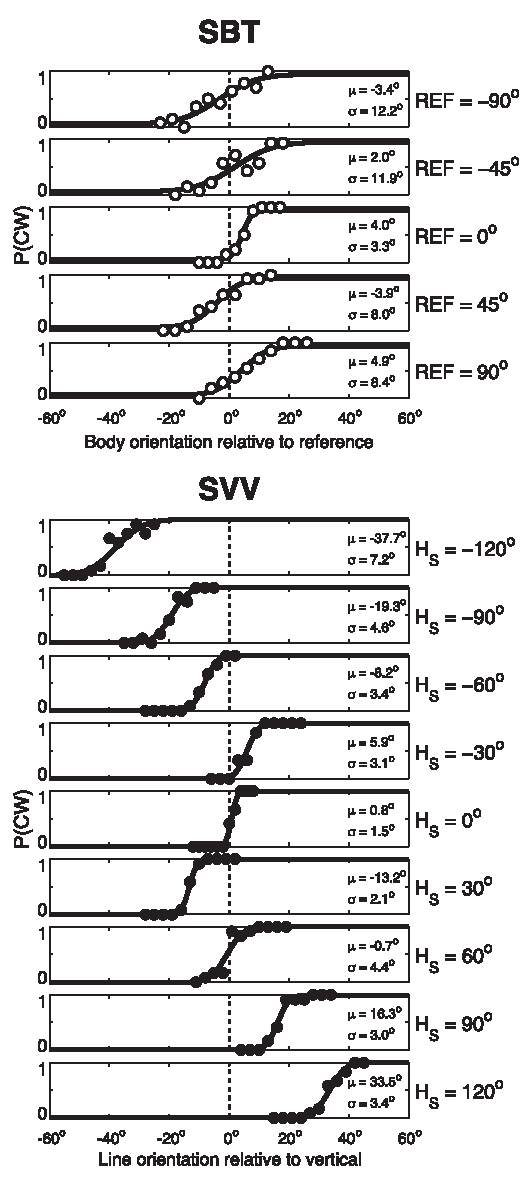
\includegraphics[width=0.5\textwidth]{src/paper1/figure3.pdf}

    \caption{SBT versus SVV performance in one subject (S1). Top, SBT. Proportion of CW responses is plotted against body orientation relative to the reference orientation (0 \si{\degree}, \textpm45 \si{\degree}, or \textpm90 \si{\degree}). $\mu > 0\degree$ indicates tilt underestimation. Bottom, SVV. Proportion of CW responses is plotted against line orientation relative to vertical. Solid lines, Best-fit cumulative Gaussians, typified by $\mu$ and $\sigma$.}
    \label{p1:fig3}
\end{figure}

The bottom section of \figref{p1:fig3} illustrates the performance of the same subject in the SVV task. Each panel demonstrates how the fraction of CW responses changes as a function of line orientation relative to the perceived vertical, for each tilt angle tested. Performance is very accurate in the upright condition. For moderate body tilts, i.e., 30\textdegree, this subject shows small systematic errors, indicating that the line must be set in a direction opposite to the head tilt to be perceived vertical in space. For larger tilts ($\ge 60$), systematic errors occur with increasing tilt angle, with amplitudes up to 40 \si{\degree}, as if tilt is underestimated. This response pattern is consistent with previous literature \cite{aubert1861, udodehaes1970, mittelstaedt1983, vanbeuzekom2000}. Close scrutiny also reveals that the precision in the vertical percept deteriorates away from the upright position.

Psychometric fits capture these observations. In the upright position, the percept of visual vertical is virtually unbiased, as indicated by a $\mu$ value of 0.8\textdegree. At large tilts, e.g., at \siang{-120} and 120\textdegree, $\mu = -37.7\degree$ and $\mu = 33.5\degree$, respectively, which means that the line must be tilted away from true vertical to be perceived as vertical in space. Furthermore, the fitted psychometric curves are steepest at \siang{0} tilt, reflected by $\sigma = 1.5\degree$. With larger tilt angles, $\sigma$ increases, reaching maximum values of 7.2 \si{\degree} and 4.3 \si{\degree} at tilts of -120 \si{\degree} and +120 \si{\degree}, respectively.

The results of this subject are exemplary for all subjects, as shown by the bias and SD data points in \figref{p1:fig4}. The mean results across the seven subjects are shown in the rightmost column. The bold lines in \figref{p1:fig4} represent the fits from our Bayesian model, which will be discussed later in this section.

\begin{figure}
	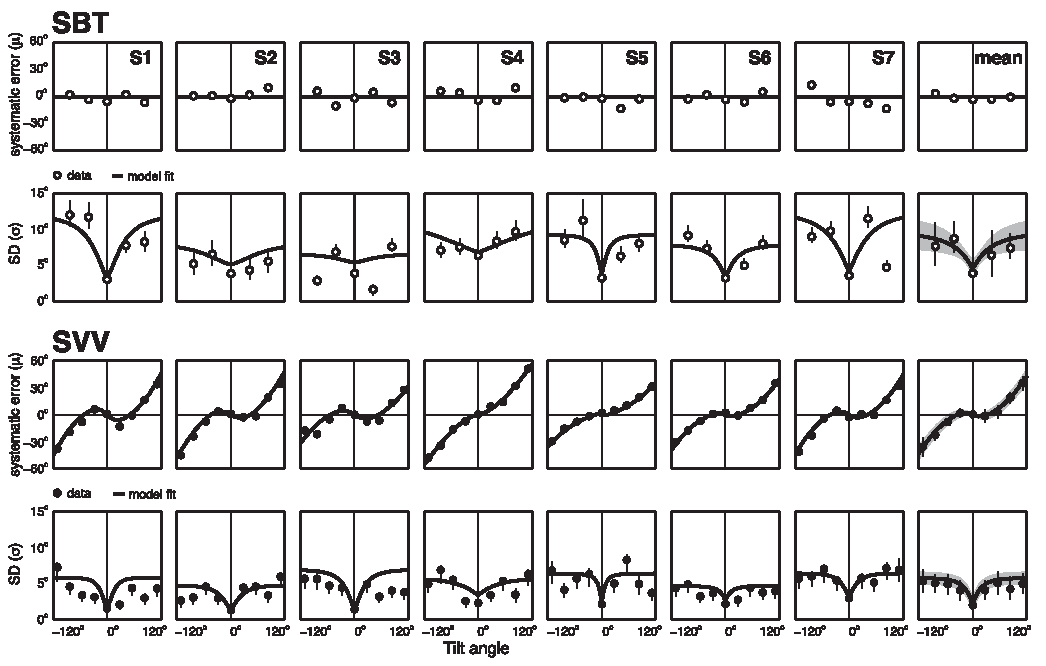
\includegraphics[width=1.0\textwidth]{src/paper1/figure4.pdf}

    \caption{Model predictions superimposed on parameters from the psychometric fits to the SBT (two top rows) and SVV data (two bottom rows). Accuracy and variability characteristics as a function of roll-tilt angle are shown; values are psychometric fits ($\mu$ and $\sigma$ values, $\circ$) and model predictions (line) from all subjects. Mean data and mean predictions across subjects are plotted in the rightmost column.}
    \label{p1:fig4}
\end{figure}

The two top rows in \figref{p1:fig4} show the accuracy ($\mu$) and precision ($\sigma$) of SBT percepts, now plotted against body orientation. For each subject, these values ($\mu$ and $\sigma$) were derived from the fitted cumulative Gaussian curves (\figref{p1:fig3}). Biases for SBT, shown in the top row of \figref{p1:fig4}, indicate moderate deviations in either direction from perfect performance, but no systematic pattern emerges. Across the seven subjects, the $\mu$ values ranged from \siang{-14.2} to \siang{+11.7} across the five SBT tasks. On average, however, there was no systematic bias for the five body orientations (ANOVA; F(4,24) = 1.4; $p = 0.25$), as also indicated by the rightmost panels. The data further show that, in all subjects, variability is statistically lower ($p < 0.05$) at the upright orientation, with $\sigma$ values \textless4\textdegree, than in the tilted conditions (\siang{45} and 90\textdegree), with $\sigma$ values ranging up to ~12\textdegree.

The two bottom rows of \figref{p1:fig4} summarise our SVV data across the entire tilt range. Accuracy is close to perfect at upright orientation in all subjects, with mean values ranging between \siang{0.1} and 2.8\textdegree. For tilts $\ge60\degree$, all subjects show systematic SVV errors (biases) of undercompensation, ranging up to maximum values close to 60\textdegree. Three subjects (S1, S2, and S3) also show slight errors of overcompensation in the smallest tilt range (\textless60\textdegree). The variability in the SVV is \siang{\textless3.0} for upright, which is consistently lower than in the tilted conditions, where variability reaches values ranging up to 8\textdegree.

Together, the results in \figref{p1:fig4} show that SVV and SBT have different accuracy and precision characteristics. Subjects perceive their body-tilt angle more accurately than the spatial orientation of the visual line. However, when it comes to variability, performance is reversed: SVV curves are narrower than the SBT curves in all subjects, at both tilt angles, meaning that they are consistently less variable in the SVV task than in the SBT task.

\subsection{Model predictions}

The bold lines in \figref{p1:fig4} present the predictions of the Bayesian integration model, fitted simultaneously to the original responses from the SBT and SVV tasks. The rightmost column of \figref{p1:fig4} shows the mean predictions from this model superimposed on the averaged parameters from the psychometric fits, indicating that the sensory integration model can account very well for all the characteristics of the data.

By design (see \nameref{p1:sec:methods}, the sensory integration model fits a horizontal fit line through $\mu_{SBT} = 0\degree$ because it cannot account for the small systematic SBT errors. As to SBT precision, the model predictions show an increase of noise with tilt angle similar to the actual increase of noise between \siang{0} and \siang{90} tilt, for all subjects. These model fits further suggest that the increase of SBT noise is steepest at small tilt angles and levels off at larger tilts. According to the model, the increase of SBT noise with tilt angle is attributable to the corresponding increase of noise in the head sensors (parameter $a_{HS}$), but levels off by the constant noise level in the body sensors. The third row in \figref{p1:fig4} depicts the model predictions of the systematic SVV errors, which show a very good match. Also with respect to SVV variability, fits and data show similar trends, suggesting an increase of SVV noise with tilt angle, which levels off at larger tilts.

For each subject, best-fit parameter values and their bootstrap-based SD levels are listed in \tabref{p1:tab1}. Parameter $b_{HS}$, representing the noise ($\sigma_{HS}$) in the otolith signal in the upright subject, ranges between \siang{1.1} and \siang{3.9}. Best-fit values of parameter $a_{HS}$ are significantly positive ($p < 0.05$) for all subjects, ranging from \siang[/\degree]{0.07} (S4) to \siang[/\degree]{0.23} (S1). This implies that the noise in the otoliths increases with tilt angle. The width of the head-in-space prior ($\sigma_{HSP}$) ranges from \siang{9.4} (S2) to \siang{18.7} (S5), with a mean of 12.5 \textpm \siang{3.2}, consistent with our previous report \cite{devrijer2009}. Best-fit values of parameter $\sigma_{BS}$, reflecting the noise in the sensory body-in-space signal, range from \siang{6.7} (S3) to \siang{15.0} (S5), with a mean of 10.8 \textpm \siang{3.1}, which is about twice as large as the best-fit values of parameter $\sigma_{HB}$, reflecting noise in the head-on-body signal, ranging from \siang{1.8} (S6) to \siang{9.3} (S3), with a mean of 4.9 \textpm 2.7\textdegree. Thus, the parameter fits imply that the neck sensors are more precise than the body-tilt sensors. As has been discussed extensively in our previous paper \cite{devrijer2009}, the amplitude of uncompensated ocular counterroll ($A_{OCR}$) shows large inter-subject variability.

\begin{table}

\begin{tabular}{lllllll}
\hline
Subject & $a_{HS}$ (\textdegree/\textdegree) & $b_{HS}$ (\textdegree) & $\sigma_{HSP}$ (\textdegree) & $\sigma_{BS}$ (\textdegree) & $\sigma_{HB}$ (\textdegree) & $A_{OCR}$ (\textdegree) \\
\hline
S1 & 0.23 \textpm 0.02 & 1.2 \textpm 0.32 & 11.6 \textpm 1.0 & 12.3 \textpm 1.1 & 3.3 \textpm 1.2 & 27.0 \textpm 2.2 \\
S2 & 0.12 \textpm 0.02 & 1.2 \textpm 0.52 & 9.4 \textpm 1.1 & 8.4 \textpm 2.9 & 6.4 \textpm 4.1 & 17.0 \textpm 3.8 \\
S3 & 0.20 \textpm 0.03 & 1.1 \textpm 0.42 & 14.4 \textpm 1.7 & 6.7 \textpm 1.9 & 9.3 \textpm 2.4 & 17.5 \textpm 2.1 \\
S4 & 0.07 \textpm 0.50 & 3.9 \textpm n/a & 11.2 \textpm 1.3 & 12.6 \textpm 2.3 & 7.1 \textpm 3.5 & 0 \textpm n/a \\
S5 & 0.11 \textpm n/a & 3.3 \textpm 1.0 & 18.7 \textpm 4.8 & 15.0 \textpm n/a & 3.6 \textpm 2.1 & 1.06 \textpm n/a \\
S6 & 0.23 \textpm 0.09 & 3.0 \textpm 1.5 & 9.5 \textpm 1.1 & 8.0 \textpm 0.83 & 1.8 \textpm n/a & 18.8 \textpm 4.1 \\
S7 & 0.20 \textpm 0.14 & 3.2 \textpm 1.0 & 12.8 \textpm 2.4 & 12.7 \textpm 6.1 & 3.0 \textpm n/a & 20.8 \textpm 9.0 \\
Mean & 0.16 \textpm 0.06 & 2.4 \textpm 1.2 & 12.5 \textpm 3.2 & 10.8 \textpm 3.1 & 4.9 \textpm 2.7 & 14.6 \textpm 10.2 \\
\end{tabular}

\caption{Best-fit parameter and bootstrap-based SD values. Imposed fit limits were as follows: $a_{HS}$: 0.5\textdegree/\textdegree; $b_{HS}$, $\sigma_{HSP}$, $\sigma_{BS}$, $\sigma_{HB}$, 50\textdegree; $A_{OCR}$, 30\textdegree. SD values are not shown (n/a) when bootstrapped values formed a skewed distribution. $a_{HS}$, Tilt-related increase in otolith noise; $b_{HS}$, otolith noise in upright position; $\sigma{HSP}$, width of head-tilt prior; $\sigma{BS}$, noise in body-in-space sensors; $\sigma{HB}$, noise in neck sensors; $A_{OCR}$, uncompensated ocular counterroll.}
\label{p1:tab1}
\end{table}

\subsection{Sensory weights}

To obtain the model fits in \figref{p1:fig4}, we made the assumption (see Introduction) that information from both direct and indirect pathways (\figref{p1:fig1}) is used to estimate body and head orientation in space. The sensory weights, indicating the relative contribution of both pathways, can be computed from the fit results in \tabref{p1:tab1}. To obtain the body-in-space estimate, necessary for the SBT, the model uses both direct information from the body sensors and indirect information from the combination of otolith and neck information. Because the variability of the otolith signal ($\sigma_{HS}$) increases with tilt angle ($a_{HS} > 0$), as shown in \tabref{p1:tab1}, the relative importance of direct and indirect pathways becomes dependent on tilt angle. This can be seen in \figref{p1:fig5} (top row), which shows the relative weights of these signals for each subject, derived from \eqnref{p1:eqn2} and the best-fit parameter values in \tabref{p1:tab1}. The mean (\textpm SD) pattern across subjects is shown in the rightmost pattern.

\begin{figure}
    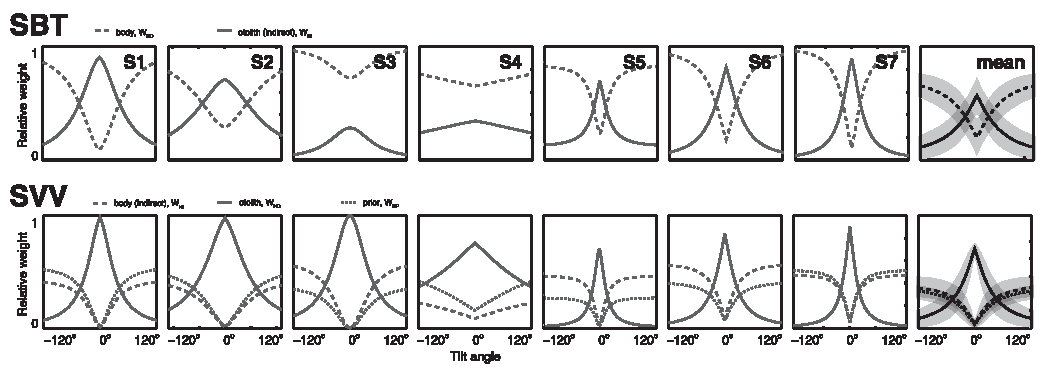
\includegraphics[width=1.0\textwidth]{src/paper1/figure5.pdf}

    \caption{Tilt dependence of weight factors in SBT (top) and SVV (bottom) for each subject. Trends with tilt angle are similar for all subjects. Head-in-space prior is only involved in SVV computations. Means across subjects are plotted in the rightmost column.}
    \label{p1:fig5}
\end{figure}

Instead of an overall dominance of body receptors in the direct pathway, the model implies that it is actually the indirect pathway, carrying the otolith signal, that dominates the behaviourally important range near upright. In most of our subjects (S1, S3, S5, S6, and S7), it was only when the otoliths became less reliable, at larger tilts, that the body sensors (direct pathway) got the upper hand ($w_{BD} > 0.5$).

For the SVV task, the model assumes that both information from the otoliths (direct) and the combination of body and neck information (indirect) is used. \figref{p1:fig5} (bottom row) illustrates the relative contributions from these sensors as well as from the prior, based on the model fits (\tabref{p1:tab1}) and \eqnref{p1:eqn6}. The SVV pattern looks similar to the SBT pattern (\figref{p1:fig5}, top row): in all subjects, the otoliths are very dominant near upright, with weights close to 1, but their contribution declines when tilt angle increases. As we saw for the SBT signal weights, this decline reflects increasing otolith noise levels. In the SVV, the decline is steeper than in the SBT, where the reference frame transformation leads to an enhanced noise level with a less pronounced tilt dependence. As the otolith contribution decays, the contributions of the prior and indirect pathway become more manifest. According to our model fits, the weight of the body sensors in the SVV task ($w_{HI}$) at \siang{90} tilt ranges between 0.19 (S4) and 0.53 (S6).

\subsection{Model evaluation}

To test whether the assumption of indirect pathways in the model is warranted, we compared its performance with a reduced version with only direct pathways (see \nameref{p1:sec:methods}). With this in mind, we performed a likelihood ratio test of the complete model fit (with direct and indirect pathways) versus the fit of a model with direct pathways only [i.e., SVV just based on head sensors (the otoliths), the SBT just based on body sensors]. The results are shown in \tabref{p1:tab2}. For each subject, the complete model provided a significantly better account of the data than the reduced model without multisensory integration through the indirect pathways. In other words, head, neck and body sensors all contribute to both SBT and SVV.

\begin{table}
\begin{tabular}{llllll}
\hline
Subject & MLE full model & MLE reduced model & $p$ & BIC full model & BIC psychometric fits \\
\hline
S1 & 231.5 & 312.4 & \textless 0.001 & 498.1 & 540.3 \\
S2 & 197.8 & 216.9 & \textless 0.001 & 430.6 & 539.3 \\
S3 & 267.5 & 313.4 & \textless 0.001 & 570.0 & 548.2 \\
S4 & 207.5 & 218.2 & \textless 0.001 & 450.0 & 569.1 \\
S5 & 195.6 & 216.3 & \textless 0.001 & 426.2 & 571.0 \\
S6 & 163.5 & 183.2 & \textless 0.001 & 362.0 & 502.5 \\
S7 & 248.0 & 260.0 & \textless 0.001 & 531.1 & 633.5 \\
\end{tabular}
\caption{Validation of the model. Log-likelihood ratio test of the full model (with indirect pathways) and reduced model (without indirect pathways). For all subjects, the full model outperforms the reduced model lacking multisensory integration through the indirect pathways. BIC values are much lower for the Bayesian integration model compared with separate psychometric fits in six of seven subjects.}
\label{p1:tab2}
\end{table}

We also compared our model, which provides a mechanistic explanation of the full dataset, with the pure descriptive account of the data as obtained by fitting separate psychometric curves to the data for the five SBT angles and nine SVV angles (\eqnref{p1:eqn1}, \figref{p1:fig3}, and \nameref{p1:sec:methods}, Model evaluation). Maximum-likelihood estimates were calculated and corrected for the number of free parameters using the BIC. As shown in \tabref{p1:tab2}, we found the lowest BIC values, indicating a better model, for the Bayesian model in all subjects, except S3. One might argue that the mean corrections before fitting the Bayesian model added another nine parameters that should be taken into account when comparing the models, even though these parameters were not fitted by the model. However, even for the worst-case scenario of 16 parameters, our Bayesian model still outperformed the individual psychometric fits ($\text{BIC}_\text{mechanistic} = 3583 < \text{BIC}_\text{psychometric} = \text{3910}$).

\subsection{Model validation}

To further validate the model, we independently tested one of its predictions that can be assessed experimentally in isolation: head-on-body variance. In supine position, subjects judged their head orientation (CW/CCW) relative to the body midline after it had been passively roll-rotated with speeds subthreshold for the canals to various angles (see \nameref{p1:sec:model:necknoise}). Psychometric fits indicate no systematic bias in these head-on-body percepts (data not shown). Figure \ref{p1:fig6} depicts the experimental noise levels derived from these psychometric fits and the predicted values provided by the model, including their 95\% confidence intervals. Because the variance of the estimates increases with the average head-on-body percept, we performed a regression on the log-transformed data \cite{hopkins2000}. The significant correlation between predicted and measured neck noise levels (slope, 1.03; intercept, -0.1; $p = 0.04$) provides an independent confirmation of the proposed model.

\begin{SCfigure}
    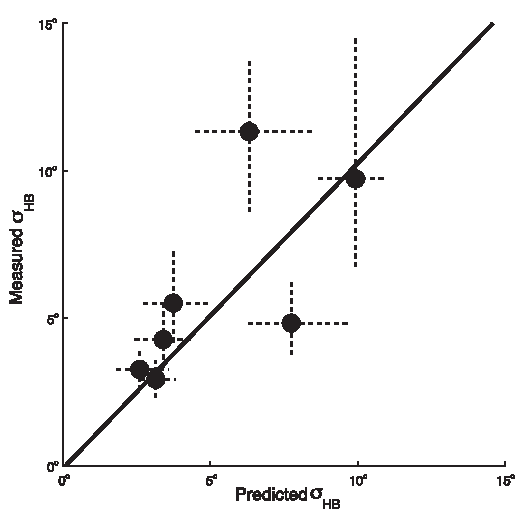
\includegraphics[width=0.35\textwidth]{src/paper1/figure6.pdf}

    \caption{Model validation. Independent measurement of neck (head-on-body) noise ver- sus the values predicted by the model. The dots represent the median values and the dashed lines the 95\% confidence interval determined from a bootstrap. Note that the variance of the estimates increases with the mean value. The solid line shows the regression based on log-transformed data (slope, 1.03; $p = 0.04$).}

    \label{p1:fig6}
\end{SCfigure}


%%%%%%%%%%%%%%
% Discussion %
%%%%%%%%%%%%%%

\section{Discussion}

In this study, we made intra-subject comparisons of the accuracy (bias) and precision (inverse variance) characteristics in two spatial orientation tasks: SBT and SVV. The main experimental findings were as follows: (1) the SBT is more accurate than the SVV, (2) the SBT is less precise than the SVV, and (3) both SBT and SVV precision are smaller in tilted conditions than near upright. Under the assumption of optimality, a Bayesian model of sensory integration could account very well for these findings. Independent measurements, in supine subjects, of head-on-body variance confirmed the predicted value.


\subsection{Comparison with previous work}

A world-vertical visual line appears tilted in space when the head is tilted in a darkened room \cite{aubert1861}. Mittelstaedt \citeyear{mittelstaedt1983} was the first to emphasise that this phenomenon cannot be explained by errors in the body-tilt percept. He showed that subjects could accurately adjust themselves to a horizontal position, but, once in this position, made substantial systematic errors in the perception of visual verticality. Later, combined tests confirmed the discrepancy between SVV and SBT accuracy \cite{mast1996, jarchow1999, vanbeuzekom2000, vanbeuzekom2001, kaptein2004, vingerhoets2008}. The present study is consistent with these findings, showing substantial systematic SVV errors at tilts $\ge60\degree$ and fairly accurate SBT performance.

Compared with the abundant literature on SBT and SVV accuracy, data on their perceptual variability are scarce. In contrast to Mittelstaedt's observation \citeyear{mittelstaedt1983}, Mast and Jarchow \citeyear{mast1996} found that the SBT was much more variable than the SVV. The present study, the first to measure both SVV and SBT precision using an extensive psychometric approach, has clearly established that SBT variability is consistently higher than SVV variability, both in the upright and in the horizontal (90\textdegree) tilt position.

Furthermore, although various studies have noted that SVV variability increased at larger tilts \cite{schone1964, schone1968, udodehaes1970, vanbeuzekom2001, devrijer2008}, little is known about SBT variability as a function of tilt angle. Nelson \citeyear{nelson1968} showed that subjects were more variable when adjusting themselves to a horizontal position than to a vertical (upright) position. The present findings are consistent with these early observations.


\subsection{Implications of the model}

After earlier indications that both the otoliths and body sensors contribute to the SBT \cite{clark1963, clark1964, nelson1968}, Mittelstaedt \citeyear{mittelstaedt1997} made a quantitative assessment of their impact, using an ingeniously designed experiment. Subjects lay on their side in a horizontal centrifuge. The crux of the experiment was to vary the distance between the rotation axis and the interaural axis to equalise the opposite contributions from the otoliths and the body sensors so that the subject felt horizontal. By testing normal, paraplegic, and nephrectomised subjects, Mittelstaedt inferred how much each sensory system contributes to body-tilt perception. It was shown that, apart from the otoliths, also internal ``graviceptors'' in the trunk (such as the viscera) participate in the computation of the SBT. Later, some related studies provided evidence that the distribution of blood in the body also affects postural perception \cite{vaitl1997, vaitl2002}. According to Mittelstaedt \citeyear{mittelstaedt1998}, the weight of the somatic graviceptors to estimate horizontal body orientation in healthy subjects is \textapprox0.6 on average, with considerable inter-subject variability. His estimate seems quite compatible with our $w_{BD}$ values at \siang{90} tilt, which range between 0.35 (S5) and 0.93 (S6) (\figref{p1:fig5}).

Previous attempts to identify the separate contributions of the otoliths, neck, and body sensors on the SVV have yielded mixed results. Whereas Mittelstaedt \citeyear{mittelstaedt1998} found no evidence that the SVV was affected by the body sensors in his centrifuge experiment, other studies indicate that neck- and trunk-tilt aftereffects \cite{wade1968}, neck muscle vibration \cite{mckenna2004}, and manipulation of tactile and interoceptive body cues \cite{trousselard2004} can affect the SVV. In other words, even in the absence of direct head-in-space information from the otoliths, the brain can still obtain an estimate of head orientation in space through the indirect sensory pathway. These findings suggest that these modalities operate together with the otoliths in the computation of the SVV, consistent with our model.


\subsection{Model evaluation}

The architecture of the model, as far as the reference frame transformations and the sensory integration is concerned, follows entirely from the principles of Bayesian inference. However, to account for our major findings and inter-subject differences, we made two less straightforward assumptions. First, to explain the increased variability in both tasks at \siang{90} tilt, we allowed for the possibility that the otoliths become more noisy with increases in tilt. Second, we hypothesised that prior knowledge is used in the visual vertical but not in body-tilt perception. Can these assumptions be justified on physiological and rational grounds?

One reason to assume that otolith noise depends on tilt angle is based on the fact that the utricle contains considerably more hair cells than the saccule \cite{rosenhall1972, rosenhall1974}. Because the utricle is most sensitive to tilts of \textapprox0\textdegree, whereas the saccule is most sensitive at \siang{\textapprox90} tilt \cite{jaeger2008}, this may well cause the proposed increase of otolith noise with tilt angle \cite{tarnutzer2010}. A tilt-dependent noise level of the otoliths would also help to explain why the perturbing effect of roll-optokinetic stimulation on the SVV \cite{dichgans1974, fernandez1976} and on the SBT \cite{young1975} is more pronounced at larger tilt angles and why the SVV is more strongly influenced by residual canal signals at larger tilt angles, after prolonged roll rotations \cite{lorincz2008}.

In the SVV literature, it is widely assumed that the visual vertical is determined by a weighted combination of a sensory head-tilt signal and a head-fixed reference, denoted as the idiotropic vector \cite{mittelstaedt1983}. Recently, this idiotropic vector has been reinterpreted in terms of a Bayesian prior \cite{eggert1998, macneilage2007, devrijer2008}, with which it is mathematically equivalent. Interestingly, when tested in gravity-free conditions, subjects still retain a sense of visual vertical, always aligned with their long-body axis, compatible with the idea of head-fixed prior \cite{mittelstaedt1983}. Vingerhoets et al. \citeyear{vingerhoets2008} recently found a similar phenomenon in the SVV during multiple-cycle dynamic roll rotation in normal gravity. Remarkably, when the same subjects were tested in a comparable dynamic SBT experiment, their responses showed very little bias on average, indicating that a prior is used only in the SVV and not for body-tilt estimation. To explain how this difference in computational approach might make sense, Vingerhoets et al. \citeyear{vingerhoets2008} speculated that precision is more important than accuracy for the visual system, for reasons of visual stability. Combining the sensory tilt signal with prior knowledge yields a more stable percept of visual space than can be derived from the sensory signal alone. In a recent study, Bortolami et al. \citeyear{bortolami2006} report virtually no bias in the haptically indicated vertical, which would be consistent with the suggestion that the prior plays primarily a role in visual processing. Likewise, for body-tilt perception, for which it might be less important to be precise and more useful to be accurate, the prior does not take part in this process.

\subsection{Clinical implications}

According to our model, statistically optimal performance requires the use of information from both direct and indirect pathways to estimate body and head orientation in space (\figref{p1:fig1}). Thus, if one of the sensory inputs is lost or severely disrupted, SBT and SVV performance will deteriorate, but should not completely break down due to their multimodality dependence. By setting the appropriate parameter values of the model to infinity, we simulated the model to predict SVV and SBT performance in two patient groups: bilateral vestibular patients (noise level of the otoliths set to infinity) and patients with somatosensory loss (noise level of the body sensors set to infinity). \figref{p1:fig7} shows the results of these simulations.

% FIXME: Change figure 7 such that the panels are side-by-side.
\begin{figure}
    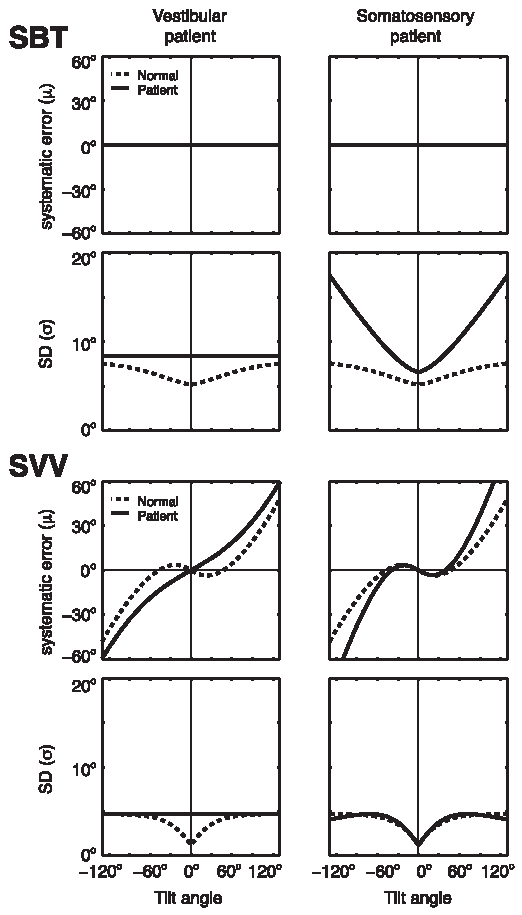
\includegraphics[width=1.0\textwidth]{src/paper1/figure7.pdf}

    \caption{Clinical implications of the model. The model simulates the SBT and SVV in a vestibular patient by raising the level of the otolith noise to infinity, keeping the other parameters at the mean values of \tabref{p1:tab1}. A somatosensory patient is modelled by setting the noise level of the body sensors to infinity. Solid lines, Patient predictions. Dashed lines, Prediction for normals.}
    \label{p1:fig7}
\end{figure}

When the otolith signal is lost (vestibular patient), the model predicts increased but constant noise levels in both the SBT and SVV, regardless of tilt angle. From the perspective of our model, the increased SBT variability can be attributed to the loss of the otolith contribution through the indirect body-in-space pathway. The increased bias in the SVV, predicted by the model, can also be understood: as the sensory-derived head-tilt estimate becomes noisier, the effect of the prior becomes more noticeable. Although there are no accuracy and variance measurements across the entire tilt range in these patients, the few previously published deficits are consistent with these predictions. Bisdorff et al. \citeyear{bisdorff1996} have shown that bilateral vestibular patients performed quite accurately in the SBT at upright, but were \textapprox40\% more variable than normal subjects. Bronstein et al. \citeyear{bronstein1996} showed that vestibular patients still compensated for their tilt angle when testing the SVV at 90\textdegree, but with a bias about twice as large as in normal subjects, consistent with our simulations.

The right column of \figref{p1:fig7} depicts a simulation of the SBT and SVV in a patient with loss of somatosensory information (somatosensory patient). In this case, the SBT depends solely on otolith information mediated through the indirect pathway. Although this signal is still accurate, it is spoiled by the larger variability of the neck signal, needed to perform the appropriate reference frame transformation. The model also predicts larger errors in the SVV in these patients than in normal subjects. Although there are no reports containing measurements of bias and variance in the SBT and SVV, paraplegic patients show that along with the otoliths, internal body sensors also contribute to the SBT if lesions are below the 12th thoracic segment \cite{mittelstaedt1997}. This evidence supports the design of our model.

In conclusion, we have tested the performance of healthy subjects in two psychophysical tasks that probe two spatial orientation estimates (SBT and SVV) and show that perceptual accuracy and precision in these tasks can be linked to the reference-frame-dependent weighting of sensory signals. We verified our theoretical framework by independent measurements of neck noise levels and by showing that it can account for the stereotypical performance of two patient groups. In this respect, our reverse-engineering approach also provides a new tool to establish diagnostic and prognostic markers of the quality of the signals involved in spatial orientation in neurological disease.


%%%%%%%%%%%%
% Appendix %
%%%%%%%%%%%%

\section{Appendix}
\label{p1:sec:appendix}

Here we provide further explanation about the Bayesian computations underlying the SVV as expressed in \eqnref[ and ]{p1:eqn6,p1:eqn10} in Materials and Methods. \figref{p1:fig8} illustrates graphically that the variance of the posterior distribution in a single trial ($\sigma^2_{\tilde{H}S}$) is not simply the same as the variance in its peak location in multiple trials, $\sigma^2(\tilde{H}_S)$. In a single trial (\panelref{p1:fig8}{A-C}), the optimal estimate of head tilt is based on the likelihood (\figref{p1:fig8}B, green curve) associated with the combined sensory input from the direct and the indirect pathway (\panelref{p1:fig8}{A}, green line, $\hat{H}_S$) and the prior (\panelref{p1:fig8}{B}, blue curve), by multiplication of the two probability distributions. The prior distribution is a Gaussian with mean $H_{SP}$ and variance $\sigma^2_{HSP}$. The peak of the resulting posterior distribution (\panelref{p1:fig8}{B-C}, orange curve) is used as the optimal estimate of head tilt ($\tilde{H}_S$), given by the following:

% Equation 13
\begin{equation}
\label{p1:eqn13}
\tilde{H}_S = w_{HS} \cdot \hat{H}_S + w_{HP} \cdot H_{SP},
\end{equation}

with

% Equation 14
\begin{equation}
\label{p1:eqn14}
w_{HS} = \frac{1 / \sigma^2_{HS}}{1 / \sigma^2_{HS} + 1 / \sigma^2_{HSP}},
\end{equation}

and

% Equation 15
\begin{equation}
\label{p1:eqn15}
w_{HP} = \frac{1 / \sigma^2_{HSP}}{1 / \sigma^2_{HS} + 1 / \sigma^2_{HSP}},
\end{equation}

in which $\sigma_{HS}$ denotes the noise in the sensory signal, known to the observer, and $w_{HS}$ and $w_{HP}$ represent the relative weights of the sensory signal and the prior, respectively. Note that \eqnref{p1:eqn13} is equivalent to \eqnref{p1:eqn1} in \nameref{p1:sec:methods}. The variance of the posterior distribution in a single trial is given by the following:

% Equation 16
\begin{equation}
\label{p1:eqn16}
\sigma^2_{HS} = w_{HS} \cdot \sigma^2_{HS} \\
              = \frac{\sigma^2_{HSP}}{\sigma^2_{HS} + \sigma^2_{HSP}} \cdot \sigma^2_{HS}
\end{equation}

and is reflected by the width of the orange curve in \panelref{p1:fig8}{B}. \panelref{p1:fig8}{D-F} illustrates performance in multiple trials, in which the posterior distributions vary due to sensory noise ($\sigma_{HS}$), whereas the prior remains fixed. The variance of each posterior distribution is fixed and is given by \eqnref{p1:eqn16}.

\begin{figure}
    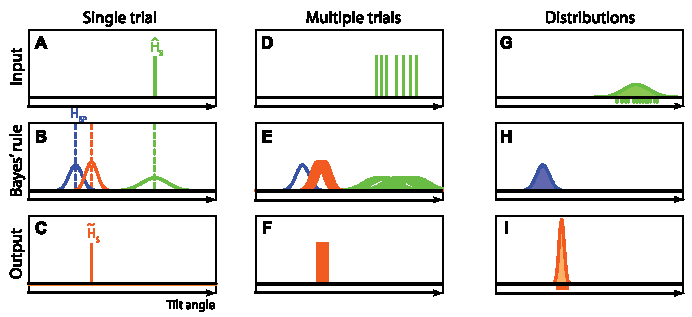
\includegraphics[width=0.80\textwidth]{src/paper1/figure8.pdf}
    \caption{Bayesian computations in single and multiple trials. \panel{A-C}, Single trial. \panel{D-F}, Multiple trials. \panel{G-I}, Resulting distributions. For further explanation, see \nameref{p1:sec:appendix}.}
    \label{p1:fig8}
\end{figure}

That the variance of the peak locations across multiple trials, $\sigma^2(\tilde{H}_S)$, is smaller can be shown by applying the rules of noise propagation to \eqnref{p1:eqn13}.

% Equation 17
\begin{equation}
\label{p1:eqn17}
\sigma^2(\tilde{H}_S) = \\
	\big( \frac{\delta\tilde{H}_S}{\delta\hat{H}_S^2} \big) \cdot \\
	\sigma^2(\hat{H}_S) + \\
	\big( \frac{\delta\tilde{H}_S}{\delta H_{SP}^2} \big) \cdot \\
	\sigma^2(H_{SP}) \\
	= w^2_{HS} \cdot \sigma^2_{HS} \\
	= \frac{\sigma^2_{HSP}}{\sigma^2_{HS} + \sigma^2_{HSP}} \cdot \sigma^2_{HS}
\end{equation}

which is equivalent to \eqnref{p1:eqn10} in Materials and Methods. Corresponding panels G-I (\figref{p1:fig8}) illustrate the distribution of the sensory signals for a given tilt angle (green-shaded curve), the prior distribution (blue-shaded curve), and the optimal estimates (orange-shaded curve), respectively. \panelref{p1:fig8}{I} illustrates that the distribution of the optimal estimates across many trials has a lower variance than the posterior distribution in each single trial (\panelref{p1:fig8}{B}), which follows from the comparison of \eqnref{p1:eqn16,p1:eqn17}, respectively.


\bibliography{refs}{}

\titleformat{\chapter}
{\normalfont\Large\bfseries}{\thechapter}{0.2em}{}
\titlespacing*{\chapter}{0pt}{-30pt}{10pt}

\end{document}


\thispagestyle{empty}

\chapter{Visual stability across combined eye and body motion}
\chaptermark{}

\vfill

\section*{Abstract}
\small
In order to maintain visual stability during self-motion, the brain needs to update any ego-centric spatial representations of the environment. Here, we use a novel psychophysical approach to investigate how, and to which extent, the brain integrates visual, extraocular, and vestibular signals pertaining to this spatial update. Participants were oscillated sideways at a frequency of 0.63 Hz while keeping gaze fixed on a stationary light. When the motion direction changed, a reference target was shown either in front or behind the fixation point. At the next reversal, half a cycle later, we tested updating of this reference location by asking participants to judge whether a briefly flashed probe was shown to the left or right of the memorized target. We show that updating is not only biased, but that the direction and magnitude of this bias depend on both gaze and object location, implying that a gaze-centered reference frame is involved. Using geometric modeling, we further show that the gaze-dependent errors can be caused by an underestimation of translation amplitude, by a bias of visually perceived objects towards the fovea (i.e., a foveal bias), or by a combination of both.

\noindent Published in the Journal of Vision \cite{clemens2012}.

\newpage

\section{Introduction}

A typical characteristic of human vision is that the position of the retina is constantly changing due to eye, head, and/or body movements. Yet, even during such self-motion, we retain a sense of whether visual objects are stable or moving with respect to an earth-centric reference frame (see e.g. Wallach, 1987). This capability is essential for a correct percept of the world and the maintenance of visual stability. 
Achieving visual stability is a complex process because visual signals are coded with respect to gaze, and not in an earth-fixed reference frame. When the visual scene lacks earth-centric landmarks, the brain should distinguish which changes in retinal input result from real world movement and which from eye movement. The usual view, dating back to Von Helmholtz (1867), is that this is achieved by subtracting the extraretinal signal of eye motion from the retinal image shifts \cite{wexler2005}.
Visual stability experiments in which participants made head-fixed saccades suggest that efference copies of the outgoing motor commands serve this purpose. Neurons in the frontal eye fields and the lateral intraparietal area demonstrate pre-saccadic shifts of receptive fields, elicited by an efference copy \cite{duhamel1992, kusunoki2003}. These gaze-centered shifts could allow the brain to anticipate and cancel out the changes in retinal input due to the saccade \cite{sommer2006}. Also, fMRI studies have reported evidence for shifting receptive fields in the human brain \cite{medendorp2003a}. 
Despite these important insights, head-fixed saccades are only one of a multitude of movements that are made in real life. Bringing the body in motion, like when driving a car, puts severe challenges on the mechanism underlying visual stability. In this case, when the body is translated passively, vestibular feedback informs the brain about the motion. This information must be combined with efference copies of orbital eye movements to interpret the changes in retinal input. Solving this problem is geometrically complicated because, during eye and body motion, the changes in retinal input depend nonlinearly on the depth and direction of objects that make up the retinal image, as in motion parallax \cite{medendorp2003b}.
Recent studies have reported fairly accurate reach or gaze responses to memorized target locations, presented prior to whole-body translations (see for review: Klier and Angelaki, 2008; Medendorp, 2011). However, such studies do not map one-to-one to the mechanisms of visual stability. First, the requirement of a motor response may invoke different processing mechanisms, which may be subject to different constraints. Second, motor response studies probe the system after the limb or eye movement, thereby revealing the combined result of all intervening spatial computations and transformations needed to guide the action. 
In the present study, we investigate visual stability across simultaneous eye and whole-body motion without involving the motor system. To this end, we used a two-alternative forced choice (2-AFC) psychophysical approach in combination with a visual updating paradigm. Participants had to retain object locations during sinusoidal whole-body motion, while keeping their gaze fixed on a world stationary point either in front of or behind the object.
By systematically manipulating the parameters of retinal and extraretinal signals related to body translation, binocular fixation, and object location, we test how the brain integrates these signals for the maintenance of visual stability. Our results show consistent errors in visual stability, which strongly depend on the location of the object relative to gaze. Using a modeling approach, we explore possible causes underlying these gaze-centered updating errors.


\section{Methods}

\subsection{Participants}

Eight participants (4 male, 4 female), aged between 22 and 41 years, provided written informed consent to participate in the experiment. All participants were free of any known vestibular or neurological disorder and had normal or corrected-to-normal visual acuity. Three participants (the authors) were knowledgeable about the purpose of the experiment, but their results did not differ from the five na�ve subjects. Participants never received any feedback about their performance.

\subsection{Setup}

A linear sled on a 800mm track was used to laterally translate participants. The sled, powered by a linear motor (TB15N, Technotion, Almelo, The Netherlands), was controlled by a Kollmorgen S700 (Danaher, Washington DC, USA) drive. The kinematics of the sled were controlled with an accuracy better than 34 ?m, 2 mm/s, and 150 mm/s2. The sled was configured such that participants were seated on the sled with the interaural axis aligned with the motion axis. Participants were restrained using a 5-point seat belt and a chin rest. In addition, the head was firmly held in place using an ear-fixed mold.  Emergency buttons at both sides of the sled chair enabled subjects to stop the sled motion immediately if needed. Eye movements were recorded using an EyeLink II (SR Research, Kanata, Canada) eye tracking system. Its camera system, which was mounted to the sled, remained stable with respect to the head during the entire experiment. Eye positions were calibrated based on the visual fixations during the experiment, under the assumption that these fixations were accurate.

\subsection{Visual stimuli}

Participants had to memorize the location of a earth-centric visual target (reference, R) during half a period of sinusoidal body translation. We tested the quality of this memory by asking them to judge and report the position of a probe stimulus (P) relative to that memorized location, following a psychophysical procedure. The reference and probe stimuli were both presented using a one-dimensional 450mm wide array, consisting of 180 red light emitting diodes (LEDs), with a spatial separation of 2.5 mm between neighboring LEDs. The LED array was oriented in parallel with the motion direction of the sled, centered w.r.t. the sled's trajectory and at the same vertical level as the participant's eyes. It was positioned with an accuracy better than 5 mm, at one of five different distances (850, 1050, 1200, 1400, or 2070 mm) from the participant's eyes in front of the sled. We further positioned an LED at either 850, 1050, 1200, 1400, or 2070 mm in front of the participant, on a virtual line orthogonal to the sled's motion direction and crossing the center of the LED array. These latter LEDs served as earth-stationary gaze fixation points (FP) during the experiment, so that gaze was directed either behind or in front of the stimulus array. The fixation points were displaced vertically by a few mm, such that the fixation point and the LED array did not occlude each other.

\subsection{Paradigm}

The experiments employed a paradigm that studies the constancy of spatial locations during 0.63 Hz sinusoidal whole-body motion in the lateral direction (left-right motion). We tested the effects of body translation (T, 150 or 300 mm peak-to-peak amplitude), fixation depth (FP, four spatial locations), and depth of the reference target (R, four spatial locations) on the quality of perceptual stability. These quantitative data will be interpreted using the geometric framework outlined in the subsection Model below.

\begin{figure}
	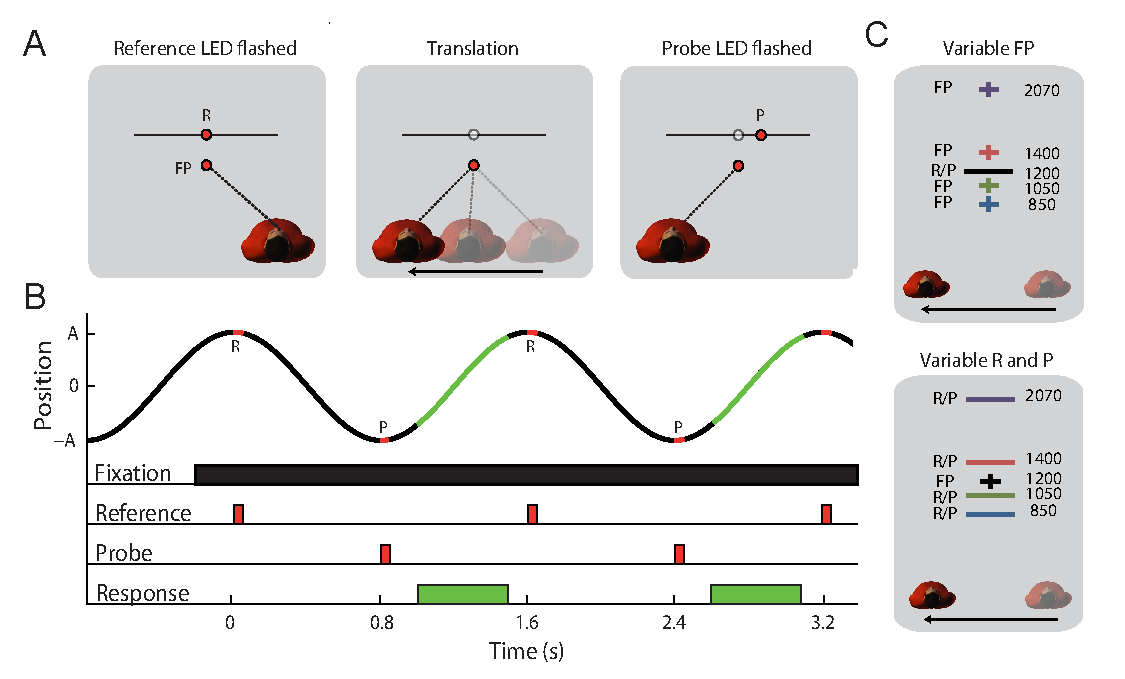
\includegraphics[width=1.0\textwidth]{src/paper2/figure1.pdf}
\end{figure}

Figure 1, panels A and B, illustrate the paradigm in detail; Figure 1C provides an overview of the experimental conditions. The experiment consisted of runs of either 30 or 15 trials. Each run started with the onset of a FP, to be fixated for the entire duration of the run. To avoid discontinuous acceleration at motion onset, sled velocity was linearly increased over one sinusoidal cycle (see Merfeld, Park, Gianna-Poulin, Black, and Wood, 2005 for a similar approach). Once the steady-state sinusoidal motion was reached, participants were tested using a visual updating task (Figure 1A). More specifically, at the most rightward position, when the body motion reversed direction, the reference R (here, the center LED) was presented for 50 ms. When the sled reached the left-most position, again during motion reversal, the participant's estimate for the location of R was tested by displaying another LED, the probe P, for 50 ms. The participant then had to report the location of this probe relative to R in a two-alternative forced choice (leftward, rightward) using a joystick. While we asked participants to respond in a timely manner, we did not explicitly constrain response time. Therefore, the next trial was only presented after a response was given. In practice, most responses were given within half a cycle (RT �SD = 0.59s �0.09, across participants). We used an adaptive algorithm to vary the spatial separation between reference and probe target from trial to trial \cite{kontsevich1999}, mapping out psychometrically the bias and precision of visual stability across whole-body motion. 
Participants were tested in 16 conditions, each comprising a unique combination of translation amplitude (T), visual fixation point (FP), and reference (R) position (see Fig 1C). The values used in this experiment are shown in Table 1. For each condition we presented 135 trials, which were divided into 4 runs of 30 trials and one run of 15 trials. In every condition 70 out of 135 trials were normal trials, that is, the central LED was used as reference. The other 65 trials in each condition were catch trials, of which 25 trials had the reference location shifted 36 mm to the left of the central led; another 25 had the reference location 36 mm rightward, and in 15 trials a random LED in the stimulus array was taken as the reference location. The catch trials were to prevent participants from simply making repeated stereotypic responses. After each run, the lights were turned on. Following a 30 s break, the experiment resumed automatically. The total experiment was divided into three sessions, tested on different days.  Each participant was tested on a total of 2160 trials.

% Table 1

\subsection{Data analysis}

To prevent effects caused by vergence and/or version eye-movements, we excluded trials in which participants did not maintain fixation within a 3 degree interval around FP, during the time interval starting 100ms before presenting the reference target and ending 100ms after cueing the probe. Overall, 6.4\% �1.7\% ({\textpm}SD) of all trials were discarded per participant based on these eye movement criteria. 
For each condition, we quantified performance by calculating the probability of a rightward response as a function of the location of the probe relative to reference location. We used a maximum likelihood fit of a cumulative Gaussian function to summarize the psychometric data:

\begin{equation}
\label{p1psych}
P(x) = \lambda + (1 - 2\lambda) \frac{1}{\sigma \sqrt{2\pi}} \int_{-\infty}^{x}{e^{-(y-\mu)^2 / 2\sigma^2}}dy,
\end{equation}

in which x represents the size of probe displacement. The mean of the Gaussian, $\mu$, represents the bias in visual stability (positive $\mu$ corresponding to a rightward bias). The width of the curve, corresponding to the standard deviation $\sigma$ of the Gaussian, is inversely related to precision, and serves as a measure of the participant's variability in the visual updating task. Parameter $\lambda$, representing the lapse rate, accounts for stimulus-independent errors caused by subject lapses or mistakes and was restricted to small values ($\lambda < 0.06$). Fits were performed using the 'psignifit' Matlab toolbox \cite{wichmann2001, wichmann2001b}.


\subsection{Model}

We investigated whether the observed bias can be explained by allowing a gain factor in the processing of the lateral translation by the vestibular system. That is, we assume that $\tilde{T} = {\alpha}T$, where $\tilde{T}$ is the perceived and $T$ the actual translation (Medendorp, Van Asselt, and Gielen, 1999). If the spatial update is performed entirely in a head-centered system, the effect of this gain would be straightforward. The reference flash $R$ is presented when the sled is in the rightmost position and the following translation of the sled by $T$ mm to the left in world coordinates amounts to a translation of the world, including the reference point, by $T$ mm to the right in head-coordinates. Due to the gain of the vestibular system the perceived translation equals ${\alpha}T$ mm to the right, leading to a predicted bias of

\begin{equation}
\mu = \tilde{T} - T = (\alpha - 1) T
\end{equation}

in mm on the LED array. Thus, when processed in a head-centered system, the bias would be negative for $\alpha < 1$, positive for $\alpha > 1$; it would be proportional to the translation amplitude, but would not depend at all on the reference and fixation point positions.
Previous experiments \cite{vanpelt2007} have shown that reach targets are updated not in head-centered coordinates, but rather within a gaze-dependent frame of reference. Following up on this, we also model the effect of the translation gain in a gaze-centered system. Let OF be the vector from the cyclopean eye to the fixation point and, similarly, $OR$ the vector to the reference point. The translation by $T$ mm to the left in world coordinates is in head-coordinates well approximated by a rotation of OF by $T/|OF|$ radians to the right and a rotation of OR by $T/|OR|$ radians to the right. (The approximation is good, since both $T<<|OF|$ and $T<<|OR|$. To express the gist of the prediction of the gaze-dependent model, this first-order approximation is very useful; in the actual calculations the precise geometry was used, without noticeable differences.)  Consequently, in gaze-centered coordinates (i.e., OF fixed straight ahead) the vector OR rotates by an angle of 

\begin{equation}
\phi \approx T (\frac{1}{|OR|} - \frac{1}{|OF|})
\end{equation}

radians to the right. In modeling the perceived rotation angle $\tilde{\phi}$ we again replace $T$ by $\tilde{T} = {\alpha}T$, but we also have to consider possible biases in the perception of $|OR|$ and $|OF|$. Following previous literature \cite{gogel1977, medendorp2003b}, we assume that the depth of the constantly visible fixation point is perceived accurately, i.e., $|\tilde{OF}| = |OF|$, but we allow that the perceived depth of the 50 ms flashed reference stimulus, $|\tilde{OR}|$, is biased towards this fixation point depth. Since the depth signals available in this experiment (vergence angle and disparity) express more directly in terms of inverse depth than depth itself. The simplest way to implement such a bias is to model the perceived reference depth as a weighted harmonic mean of the actual reference and fixation depths:

\begin{equation}
\frac{1}{|\tilde{OR}|} = \beta \frac{1}{|OR|} + (1 - \beta) \frac{1}{|OF|}
\end{equation}

where $\beta = 1$ represents the limiting case of accurate depth perception of the reference stimulus (no bias) and $\beta = 0$ the limiting case of full "assimilation" to fixation point depth. In total this leads to a perceived rotation angle of

\begin{equation}
\tilde{\phi} = {\alpha}T \cdot \beta(\frac{1}{|OR|} - \frac{1}{|OF|})
\end{equation}

radians to the right. Comparing Eq. 5 with Eq. 3 shows that our assumptions amount to a total gain of $\alpha\beta$ on the rotation angle, with freely interchangeable contributions of the parameters $\alpha$ and $\beta$. We substitute $\gamma = \alpha\beta$ and note that the resulting bias in angle, $\tilde{\phi} - \phi$, is observed as a bias in mm on the LED array at a distance $|OR|$:

\begin{equation}
\mu = (\tilde{\phi} - \phi)|OR| = (\gamma - 1)T(1 - \frac{|OR|}{|OF|})
\end{equation}

Thus, in the gaze-centered model the bias is again proportional to translation amplitude, but now it also depends critically on the fixation and reference point positions. In particular, the bias flips sign according to presenting the reference point in front of or behind the fixation point. On top of this, there is an overall (across all conditions) sign dependence on the combined values of the translation gain and fixation depth bias factors.

\section{Results}

Participants were tested in an experimental paradigm that studies the stability of spatial locations across combined eye and body motion. The task, illustrated in Figure 1, requires that subjects fixate an earth-stationary central fixation point, FP, which is visible throughout the run. At two successive reversals of motion direction, at the right and left excursion point of the sinusoidal motion, a reference (R) and a probe (P) target are briefly flashed. In a two-alternative forced choice task, the participant has to indicate whether the probe location was to the left or to the right of the reference location. The resulting psychometric data provide a quantitative assessment of the bias ($\mu$) and precision ($\sigma^{-2}$) of visual stability across self-motion (see Methods for details). Depending on the stimulus conditions (FP, R, and T), participants may erroneously judge the location of R, and hence provide biased responses.

Figure 2 shows the results of a typical participant, plotting the fraction of rightward responses (indicated by the circles) as a function of horizontal probe location relative to the reference. The 16 conditions are split into 4 panels according to the manipulated variable: FP distance (top panels), reference distance (bottom panels) and translation amplitude (left vs. right panels). Data for all individual probes are presented (circles). In an ideal observer, all psychometric functions would constitute a step response centered at zero, indicating no bias and no uncertainty. However, the actual data show consistent biases and non-zero variance.
When FP was behind R, we observed a leftward bias (top panels; red and purple curves), that increased when fixation was further away from the reference location (red vs. purple dots). When FP was in front of R (green and blue dots), the opposite pattern was seen. Furthermore, as T increases, psychometric curves move away from zero (t-test; $t(63) = -4.55$, $p < 0.05$) and become less steep (t-test; $t(63) = -4.64$, $p < 0.05$), a sign that there is decay in both accuracy and precision (compare left and right panels). Similar biases are observed when keeping FP constant, and varying the location of R, as demonstrated by the bottom panels. We derived estimates of the bias ($\mu$) and corresponding standard deviation ($\sigma$) values in each of the 16 conditions, for all subjects.

\begin{figure}
    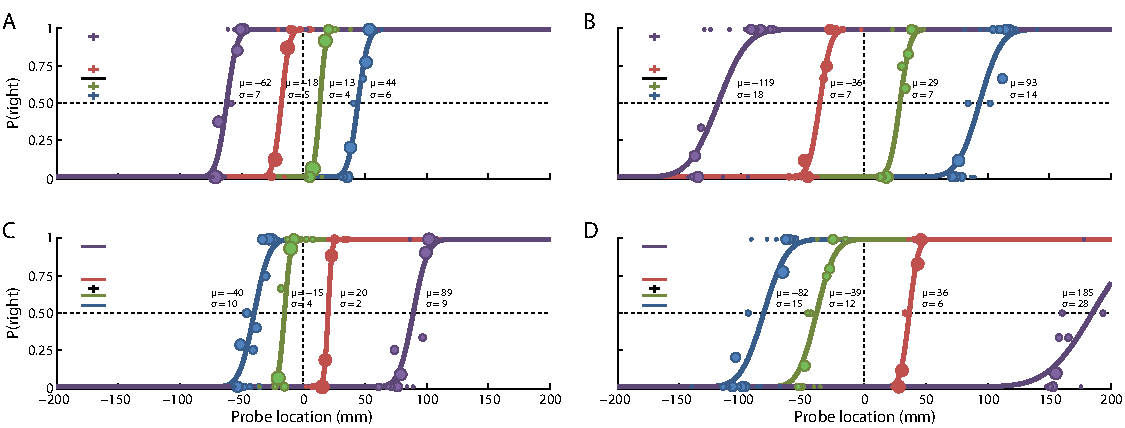
\includegraphics[width=1.0\textwidth]{src/paper2/figure2.pdf}
\end{figure}

Figure 3 depicts the bias ($\mu$) for each subject (dots), together with the mean bias {\textpm}SD across subjects (error bars), in top-view panels. This shows that the pattern in Figure 2 holds across all participants, with biases ranging between -126 and 212 mm. Clearly, the bias in updating of the central target increases with T and depends on FP, reversing for gaze fixation behind versus in front of the R (two top panels). Likewise, when FP was kept constant, the updating bias is not only larger for the larger T, but also depends on the location of R, with the bias in opposite directions for targets presented in front versus behind fixation (two bottom panels). Taken together, these observations suggest that the location of R relative to gaze, rather than the head-centric locations of FP or R, is a crucial factor in determining the updating bias. 

\begin{figure}
    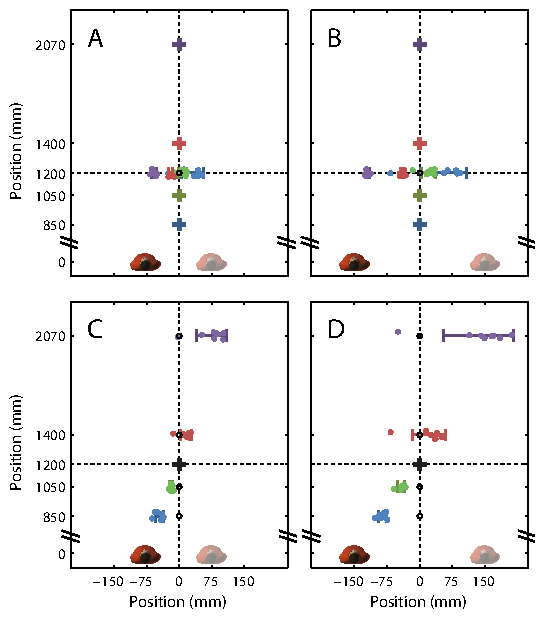
\includegraphics[width=0.75\textwidth]{src/paper2/figure3.pdf}
\end{figure}

To further analyze these observations, Figure 4 plots the bias values ({\textpm}SE across participants) as a function of gaze fixation FP (panel A), target location R (panel B) and reference location relative to gaze fixation FP - R (panel C). Both the location of FP and R, as well as the bias are expressed in units of degrees instead of millimeters because the former is more closely associated with native visual coordinates. (In practice, however, because of the large distance, visual angles are about proportional to the associated horizontal distances). While in panel A no clear relationship is observed ($R^2 = 0.09$, $F(1,14) = 1.32$; $p > 0.05$), panel B reveals only a weak linear relationship ($R^2 = 0.25$, $F(1,14) = 4.71$; $p < 0.05$). However, in panel C the data for all conditions are rearranged such that they fall into a single response curve. A linear fit shows a very strong correlation in this case ($R^2 = 0.97$, $F(1,14) = 483$, $p < 0.05$). This suggests that the observed errors almost solely depend on the location of R relative to gaze.

\begin{figure}
    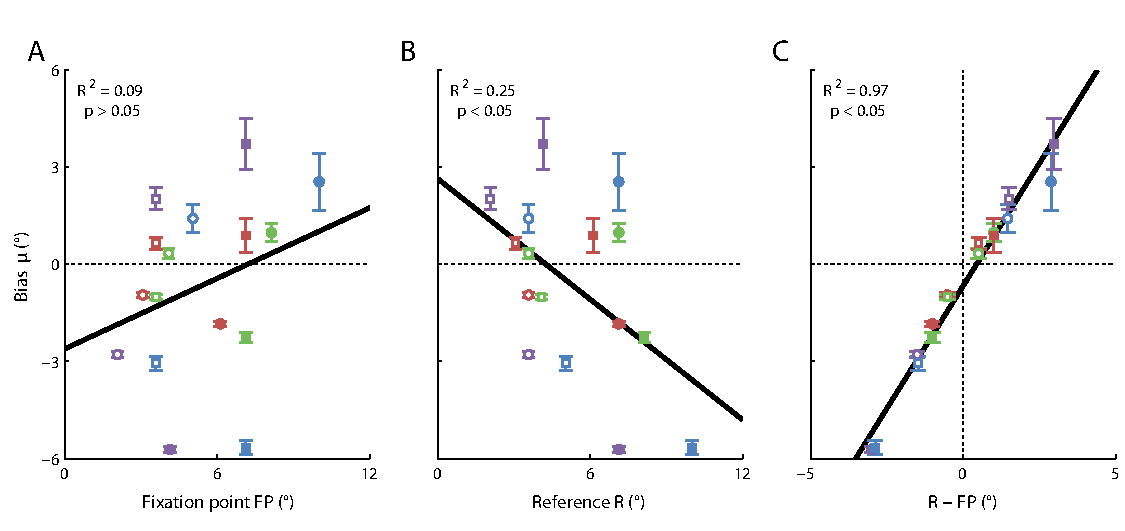
\includegraphics[width=1.0\textwidth]{src/paper2/figure4.pdf}
\end{figure}

To validate this notion, we fit two different models to explain the updating biases: a head- and gaze-centered model (see Eqs. 2 and 6 respectively, in Methods). Because the updating bias systematically depends on gaze, we expect the gaze-centered model to outperform the head-centered model. Indeed, the RMSE of the gaze-centered model was significantly lower (t-test; $t(7) = -3.68$, $p < 0.05$) than that of the head-centered model. Table 2 presents the RMSE values for both models and the fit-results of the gaze-centered model for each participant. According to this latter model, the best-fit value of the gain $\gamma$ (mean 0.25 \textpm0.08 SE) is considerably lower than the ideal value of one. In the Discussion we will address the possible implications of this small value.

% Table 2

Finally, in addition to accuracy, we also quantified the precision of the updated R. Figure 5 shows the standard deviation ($\sigma$ {\textpm}SE across participants) of the psychometric functions as a function of either FP (panel A), the head-centered location of R (panel B) or the gaze-centered location of R (panel C), in the same format as Fig. 4. No significant effects can be observed in panels A and B ($R^2 = 0.18$, $F(1,14) = 3.14$, $p > 0.05$ and $R^2 = 0.00$, $F(1,14) = 0.03$, $p > 0.05$ respectively). Panel C shows a significant linear relationship ($R^2 = 0.41$, $F(1,14) = 9.68$, $p < 0.05$). From this, we conclude that precision decreases for targets that are further or nearer in depth relative to fixation, and therefore also more peripheral in gaze-coordinates.

\begin{figure}
    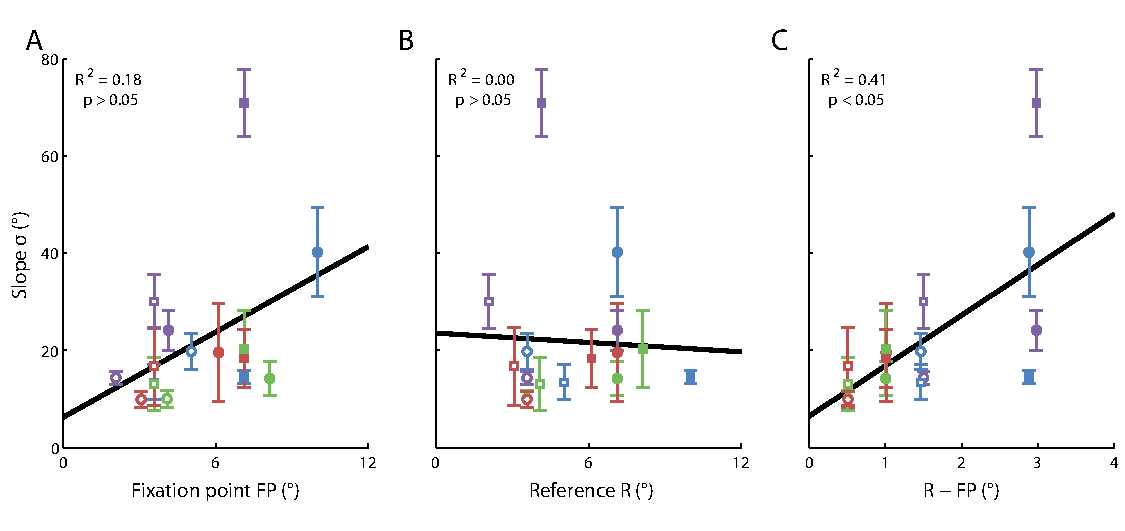
\includegraphics[width=1.0\textwidth]{src/paper2/figure5.pdf}
\end{figure}

\section{Discussion}

We investigated how the brain integrates retinal and extraretinal signals in order to maintain visual stability across combined eye and body motion. Participants had to remember the location of a world-fixed reference target, flashed in the periphery, while their body was passively translated and their binocular gaze actively changed in order to fixate a world-stationary target LED. When body motion reversed direction, a probe target was presented and the participant indicated whether it was shown to the left or right of the memorized reference. The resulting psychometric curves revealed substantial biases in the updating of the reference target, which increased with depth from fixation and reversed in sign for reference targets presented at opposite depths from fixation. In addition, precision of visual stability decreased when the distance between this target and the fixation point increased, likely due to the lower spatial resolution in the retinal periphery \cite{westheimer1982}. Geometric modeling suggests that these observations are consistent with spatial updating in a gaze-centered reference frame. In the following, we compare our results to previous work, and explore possible explanations of our observations in context of the gaze-dependent updating model.

\subsection{Relation to previous studies}

To our knowledge, there have been no other studies that have psychophysically investigated perceptual stability during combined eye and body motion. So far, related studies have tested spatial stability using paradigms in which participants make saccades or reaches to previously flashed targets after intervening self-motion (see Klier and Angelaki, 2008; Medendorp, 2011 for review). 
For actively generated self-motion, Medendorp et al. (2003b) had participants make saccade-vergence movements to remembered targets that were presented before they made a sidestep. Although their participants initially misperceived the targets, i.e. they underestimated the depths of distant targets and overestimated depths of near targets \cite{gogel1977, komoda1974, philbeck1997}, they accurately compensated for the intervening motion in the updating of the perceived target location, following the required non-linear updating patterns. Similar observations were made in relation to the updating of spatial locations across active self-motion for reaching \cite{admiraal2004, flanders1999, medendorp1999, vanpelt2007}. Compared to the present study, compensation for active intervening whole body motion was substantially better in all these studies.
Regarding passively induced self-motion, previous work by Isra\"el and Berthoz \nocite{israel1989} and more recent observations by Klier, Hess and Angelaki (2008) showed that human participants can also update the locations of saccade targets for passive whole body motion. Similar experiments in non-human primates have also demonstrated compensation for translational motion in the updating of saccadic space \cite{li2005a}. Although the amount of compensation depended on the depth of fixation, it was typically less than geometrically required (see their figure 4B), as in the present results. The same experiments were also conducted in labyrinthectomized monkeys, showing that their updating is even more compromised \cite{li2005b, wei2006}. This suggests that otolith information interacts with visual information to update saccade goals. 
Thus, in view of previous studies, our results are consistent with the notion that spatial ability is better maintained across active compared to passive body motion, perhaps due to the presence of efference copies of motor commands during active motion. Furthermore, based on the present findings it seems that perceptual updating is worse when compared to the action-oriented updating in previous studies. Should this be interpreted in favor of the proposal that visuospatial updating is organized in distinct processing pathways, one for conscious perception and one for the control of action \cite{goodale1992}? We do not want to suggest this. There may be other factors that contribute to the relatively low updating performance in the present study. Using geometric models (i.e., Eqs. 2 and 6) we will now explore such factors in more detail.

\subsection{Modeling implications}

In order to systematically explore possible explanations for the updating performance found in the present study, we now return to the head- and gaze-centered models of the updating mechanism presented in Eqs. 2 and 6 respectively. These models were inspired by the models proposed by Van Pelt and Medendorp (2007), with the addition of the possibility of a foveal bias. In the head-centered model (Eq. 2), the updating bias is proportional to the translation amplitude, but independent of reference and/or fixation point positions. However, since our data show a clear and systematic dependence on these positions (see Figs. 2-4), this model is not viable.
This leaves us with the gaze-centered model of Eq. 6, which incorporates these dependencies. Estimating the overall gain parameter ? in this gaze-centered model yielded a mean value of ? = 0.25 across participants. Since this ? is the product of parameters ? and ? (see Eq. 5), this entails that at least one of these parameters must be considerably smaller than one, the veridical value. That is, in the updating process the translation is perceived with a small gain (? << 1) and/or there is a distinct bias towards fixation depth (? << 1). We now explore the plausibility of these explanations in turn. 
For the perception of body translation at least two signals may be important: the vestibular signal from the otoliths and the changes in eye position while tracking the visual FP. Both linear acceleration (peak: 231 cm/s2) and frequency (0.63 Hz) were well above the detection thresholds of the otoliths \cite{benson1986, yu2012}. Furthermore, the firing rate of otolith afferents increases monotonically with acceleration in our frequency range \cite{fernandez1976, yu2012}, and can therefore be used to correctly decode acceleration. However, this does not mean that further processing of acceleration into a velocity or displacement signal is veridical \cite{merfeld2005}. In fact, it has been shown that the translational vestibuloocular reflex is not perfectly compensatory at the frequency that we have tested. However, when the vestibular signal is complemented by visual following mechanisms, participants are able to maintain fixation \cite{medendorp2002, paige1998}. This indicates that a near veridical percept of translation is possible by combining vestibular and eye position information. Yet, higher level processing of the translation signal might still be biased. For instance, the conversion of translated distance into an updating angle might be faulty, and/or the actual updating process itself could misinterpret an otherwise veridical updating angle. It has been shown that near-veridical updating takes place for e.g. reach targets \cite{henriques1998, vanpelt2007} where errors are attributed to the reference frame transformation instead. This suggests that the gaze-centered remapping process itself, which is thought to drive spatial updating, is not biased.
Thus, when considering previous work, it is most likely the higher level processing of the translation signal that governs the observed biases. One such processing step concerns the problem of attributing visual motion to either self-motion or object-motion \cite{vonhelmholtz1867}. If this attribution is flawed, it can have a profound influence on updating and might be the cause of our low updating gain. Support for this idea is found in work by Dyde and Harris (2008) who showed that participants make such attribution errors, in particular in conditions of passive translation and darkness, both of which apply to our study. In the active translation studies mentioned earlier, this effect is likely diminished by the presence of an efference copy that helps in disambiguating self-motion from object-motion.
A further explanation for our low overall gain is that depth perception of the reference point is biased (? << 1). Because the reference and probe lights were flashed for only 50ms at the zero velocity points of the sinusoidal motion and the head is unable to move relative to the body, depth perception of these lights is likely to be compromised. Actually, the spatial updating process that takes place in our experiment can alternatively be described in terms of a Bayesian model. To represent the brain's assumption that, lacking any precision information, the depth of peripheral stimuli is at or close to fixation point depth, such a model will involve a prior distribution centered at this fixation depth. The full specification of such a Bayesian model is beyond the scope of this paper. Here, we have opted for a more straightforward geometrical modeling approach (Eqs. 2 to 6), in which such a foveal depth bias appears in Eq. 4 with the weight 1 - ?. While such foveal influences have been reported previously \cite{brenner2008, mateeff1983}, for this to be the sole explanation for our low gain would require the foveal bias to be 80\%, which is quite extreme.
In conclusion, we have shown systematic biases in visual stability across combined eye and body movements. These biases are consistent with a gaze-centered updating model, with simple gain factors on both translation and depth perception.  


\documentclass[10pt,b5paper,twoside]{book}


%
% Common packages and custom commands used by the main .tex files.
%

\usepackage[dutch,british]{babel}
\usepackage[nottoc]{tocbibind}
\usepackage{amsmath}
\usepackage{amsfonts}
\usepackage{amssymb}
\usepackage{graphicx}
\usepackage{gensymb}
\usepackage{textcomp}
\usepackage{hyperref}
\usepackage{doi}
\usepackage{xcolor}
\usepackage{nameref}
\usepackage{xspace}
\usepackage{titlesec}
\usepackage{floatrow}
\usepackage{longtable}
\usepackage{siunitx}
\usepackage[outercaption]{sidecap}
%\usepackage{fancyhdr}
\usepackage{wrapfig}
\usepackage{lmodern}
\usepackage[font={scriptsize, sf}, labelfont={sf,scriptsize,bf}]{caption}
\usepackage{src/apacite_custom}
\usepackage{src/thesis}

\pagestyle{plain}

\floatsetup[table]{font={scriptsize, sf}}

\hypersetup{colorlinks=true, linkcolor=blue, citecolor=blue}
\setcounter{tocdepth}{2}

% Do not add extra vertical space
\raggedbottom

% Indent paragraphs
\setlength{\parindent}{1.0cm}

\bibliographystyle{apacite_custom}

\renewcommand{\baselinestretch}{1.2}
\setlength{\parskip}{0ex plus 0.3ex minus 0.3ex}

\newcommand{\about}{$\approx$}

%% For the Chapter title, etc.
\newcommand{\bigrule}{\titlerule[0.5mm]}
\titleformat{\chapter}[display]
{\normalfont\filleft\bfseries\itshape}
{%
 \vskip-3em
\titlerule[1pt]%
\vspace{1pt}%
\titlerule
\vspace{1pc}%
\Large\MakeUppercase{\chaptertitlename} \thechapter}
{1pc}
{\titlerule
\vspace{1pc}%
\thispagestyle{empty}
\Huge}


\hypersetup{
    pdfauthor = {Ivar Clemens},
    %pdftitle = {Choosing our words},
    %pdfsubject = {Language production},
    %pdfkeywords = {language production; }
}

\begin{document}

\selectlanguage{british}

\thispagestyle{empty}

\chapter{Integration of ocular and vestibular signals for self-motion perception in darkness}
\chaptermark{}

\newpage

\small {\bf Abstract} Self-motion is typically accompanied by compensatory eye movements that help minimize retinal slip and maximize dynamic visual acuity. To date, it is unknown whether these eye movements also have a reversed role, serving as a cue for self-motion perception. To address this question, we had participants ($n=8$) judge self-motion during different eye movement conditions in the absence of full-field optic flow.  In a 2-AFC task, participants indicated whether the second of two successive passive lateral whole-body translations was longer or shorter than the first. Eye movements during each translation were world-stationary, body-stationary in an otherwise dark room. Results of these two conditions show that the perceived translations were shorter with body-fixed gaze compared to world-fixed gaze. Using a linear model, we estimated the relative contributions of vestibular and eye movement signals to self-motion perception and found that eye movement signals contribute approximately 25 percent. The model was independently validated by successfully predicting the effects of eye movements on self-motion in a third condition without any visual fixation, i.e. when the eyes were free to move. We conclude that eye movement signals influence self-motion perception, even in the absence of visual stimulation, and even when oculomotor and vestibular estimates are in conflict, e.g. during body-fixed gaze. We hypothesize that adverse consequences of this seemingly inflexible arrangement are minimal under natural conditions because eye movements and self-motion are highly correlated, and because eye movements are most often accompanied by veridical optic flow cues to self-motion.

\vfill

\noindent\underline{ \hspace{4cm} }

\noindent This chapter is being prepared for publication \newline
\noindent {\bf Clemens, I.A.H.}, Selen, L.P.J., MacNeilage, P.R. and Medendorp, W.P. \citeyear{clemens2015a}. %Title. \emph{Journal}, volume(issue): from-to. \newline

\newpage

\section{Introduction}

An accurate estimate of self-motion is important to guide interactions with the environment. During passive self-motion both vestibular and optic flow signals provide information about self-motion \cite{gibson1955,benson1986,harris2000,israel1989,angelaki2005,carriot2013,chen2010}. However, also compensatory eye movements that maintain fixation on world-fixed objects carry self-motion information. These eye movements are driven by retinal slip or vestibular signals. For example, the linear vestibulo-ocular reflex (LVOR) stabilizes gaze during head translations, even in complete darkness \cite{paige1989,medendorp2002,angelaki2004}.  Many have shown that the brain uses oculomotor signals to extract the optic flow component related to self-motion \cite{warren1988,royden1992,freeman1998,lappe1999}. Here we investigate whether these oculomotor signals are also used to estimate self-motion directly.

When gaze is world-stable during whole-body translation, the eye displacement correlates with translation size and is modulated by fixation depth \cite{schwarz1989,paige1998,mchenry2000,medendorp2002}. When properly scaled this eye movement signal could serve as a self-motion cue. In contrast, when fixation is body-fixed the eyes remain stationary in their orbits \cite{paige1998,ramat2005} making them no longer informative about self-motion. If, however, the brain assumes that eye movements are always made to maintain world-stable gaze, as in the LVOR, it would equate the absence of eye movements with the absence of self-motion. As a result, self-motion with body-fixed gaze should be underestimated compared to self-motion with world-fixed gaze, despite identical vestibular cues.

In support of this notion, Guedry and Harris \citeyear{guedry1963} reported that lateral body displacements made while watching a body-fixed target, were underestimated relative to body displacements in darkness. While they explained this as a shift of attention between different sensory components, we consider the alternative hypothesis that eye movements themselves are a self-motion cue. This hypothesis implies that oculomotor signals are always combined with vestibular signals to estimate self-motion, even in complete darkness.  In this case, the size of the unconstrained eye movements should resemble a VOR movement that is intermediate between body- and world-fixed fixation, and should parametrically relate to the perceived self-motion.

To test this, we employed a two-alternative forced choice (2-AFC) paradigm in which participants were presented with two consecutive lateral translations. They had to indicate whether the second translation was longer or shorter than the first. Eye movements during each interval were free, world-stationary or body-stationary. We show that identical translations were perceived shorter when gaze was body-fixed compared to world-fixed. Furthermore, using a linear model we predicted perceived displacement during the free gaze condition based on vestibular signals and unconstrained eye movements. We conclude that eye movements influence self-motion perception even in the absence of optic flow or other visual stimulation.
\section{Materials and methods}
\label{p3:sec:methods}

\subsection{Participants}

Eight naive participants (three male, five female), aged between 22 and 29 years, provided written informed consent to participate in the experiment. All participants were free of any known vestibular or neurological disorder and had normal or corrected-to-normal visual acuity. Participants never received any feedback about their performance.

\subsection{Experimental setup}

A motorized linear sled \cite<see>[for details]{clemens2012} was used to laterally translate participants following a minimum jerk profile \cite{flash1985} of fixed duration (1 \si{\second}) and amplitudes ranging from 1 to 27 \si{\centi\metre}. Participants were seated on the sled such that the inter-aural axis aligned with the motion axis. They were restrained using a five-point seat belt and a chin rest. In addition, the head was held in place using a sled-fixed mold which resembled head-phones and pressed down on the head surrounding the pinnae. Auditory cues were suppressed using white noise presented through in-ear headphones. Experiments were conducted in complete darkness except for visual fixation points, projected by a laser pointer on a black bar 50 \si{\centi\metre} in front of the participant at eye level. Laser pointers used to project body-fixed targets were attached to the sled. Those used to project world-fixed targets were mounted on the wall behind the sled.

Eye movements were recorded at 500\si{\hertz} using an EyeLink II system (SR Research, Kanata, Canada) whose cameras were mounted to the sled and therefore remained stable with respect to the head during the entire experiment. Because the head and body positions were fixed during the experiment, the orientation of the eyes within the head, as measured by the tracker, was equivalent to the orientation of the eyes in space. The eye tracking system was calibrated before each session using 11 evenly spaced calibration points ranging from -22 to \siang{22} degrees. We used linear regression to link EyeLink measurements to gaze angles.

\subsection{Paradigm}
We used a two-alternative forced choice (2-AFC) task to measure perceived linear self-motion across three different eye fixation types: world-fixed, body-fixed, and unconstrained (free) fixation. We refer to these as world, body and free, respectively. A trial contained two sequential translation intervals of equal duration (1 \si{\second}) and in the same direction (either leftward or rightward). Different fixation types were presented in the two translation intervals. Participants were instructed to judge whether the translation during the second interval was longer or shorter compared to the first interval. They were additionally instructed to always look at the fixation point when it was visible; no instructions were given for when the fixation point was switched off (i.e. during free fixation).


\begin{figure}
    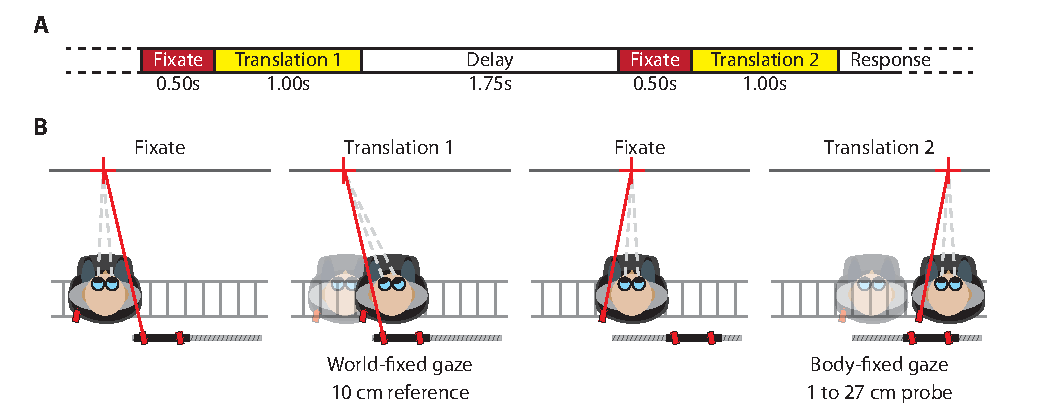
\includegraphics[width=1.0\textwidth]{src/paper3/figure1.pdf}

    \caption{\panelref{A} Time course of key events within a single trial. In each of the two intervals, a 0.50 \si{\second} fixation period (red) precedes the lateral translation (yellow). A 1.75 \si{\second} long delay period (shown in white) separates the two intervals. After the second translation, the participant responded whether this second translation was longer or shorter than the first. \panelref{B} Top-view illustrating key events during a body vs. world trial. First panel: participant fixates the world-fixed target (red cross) at the start of the first interval. Second panel: translation with world-fixed fixation target. Third panel: body-fixed fixation at start of second fixation interval. Fourth panel: translation with body-fixed fixation in second interval.}
    \label{p3:fig1}
\end{figure}

The time evolution of a single trial is shown in \figref{p3:fig1}. Each trial started with the onset of a central fixation point (i.e. aligned between the eyes) for 0.5 \si{\second}. Subsequently, the first translation interval commenced.  Depending on the fixation type, the fixation point remained visible (world and body) or was extinguished (free) during the translation interval. The trial shown in the figure depicts the 10 \si{\centi\metre} reference translation with world fixation. After this first interval, a delay followed in which the participant was kept in complete darkness for 1.75 \si{\second}. Then, the central fixation point reappeared, followed 0.5 \si{\second} later by the second interval, in which the probe translation was presented. The set of possible probe translations ranged from 1 to 27 \si{\centi\metre} in equidistant steps of 0.4 \si{\milli\metre}. The fixation type in the probe interval was always different than in the associated reference interval (the trial in \figref{p3:fig1} illustrates body fixation). After the second interval, the participant had to indicate whether he or she perceived the second translation as longer or shorter than the first using a 1-dimensional joystick. Moving the poke away from the body indicted that the second movement was longer, while moving it towards the body indicated that the second movement was shorter.


\begin{table}
    \begin{tabular}{llll}
    Comparison & Reference & 1st interval & Direction \\
    \hline
    Body vs. world & Body & Reference & Right \\
    & & & Left \\
    & & Probe & Right \\
    & & & Left \\
    \cline{2-4}
	& Body & Reference & Right \\
    & & & Left \\
    & & Probe & Right \\
    & & & Left \\
    \hline
    Body vs. free & Body & Reference & Right \\
    & & & Left \\
    & & Probe & Right \\
    & & & Left \\
    \cline{2-4}
	& Free & Reference & Right \\
    & & & Left \\
    & & Probe & Right \\
    & & & Left \\
    \hline
    World vs. free & World & Reference & Right \\
    & & & Left \\
    & & Probe & Right \\
    & & & Left \\
    \cline{2-4}
	& Free & Reference & Right \\
    & & & Left \\
    & & Probe & Right \\
    & & & Left \\
    \end{tabular}

    \caption{List of the three main comparisons that we tested. The (10 \si{\centi\metre}) reference movement was presented in either the first or second movement interval. We also manipulated movement direction (leftwards or rightwards), yielding a total of 24 trial types.}

    \label{p3:tab1}
\end{table}

Thus, a trial consists of two translations with different fixation types; in the three main conditions we compare the body versus world, world versus free, and body versus free fixation types. For each main condition, we varied which fixation type served as the reference stimulus and the order in which reference and probe were presented, which gives a total of four variations per main condition (see \tabref{p3:tab1}). In addition we varied translation direction (either leftward or rightward on consecutive trials). The amplitude of the probe translation was adaptively chosen using the Psi method. This method picks the amplitude for the next trial which maximizes the expected decrease in entropy based on participants' responses to earlier trials \cite{kontsevich1999}. This was done separately for all 24 trial types (3 main conditions x 2 reference stimuli x 2 reference/probe orders x 2 translation directions; see \tabref{p3:tab1}). A total of 25 trials were collected per trial type yielding a total of 200 trials for each of the three main conditions.

Trials were presented in three one-hour sessions. To prevent dark adaptation, we turned on the lights for 5 \si{\second} after every block of 6 trials, and for at least 30 \si{\second} every 4 blocks. We made sure that each of the 24 unique trial types were presented once every 4 blocks. After each block, the adaptive procedure determined which translation amplitudes to test in the following block. To increase the number of data-points available to the adaptive psychometric procedure at the beginning of the experiment, we collapsed across translation direction and reference order for the first 10 trials of every condition. After those collapsed trials, the procedure ran separately for each of the 24 distinct trial types.

\subsection{Data analysis}

For each combination of the three main conditions, and  the two reference/probe orders (see \tabref{p3:tab1}), we quantified the perceived probe translation  by calculating the probability of the probe translation judged longer compared to the 10 \si{\centi\metre} reference translation as a function of actual probe translation, given by x. We used a maximum likelihood fit of a cumulative Gaussian function to summarize the psychometric data:

\begin{equation}
\label{p3:eq1}
P(x) = \lambda + (1 - 2\lambda) \frac{1}{\sigma \sqrt{2\pi}} \int_{-\infty}^{x}{e^{-(y-\mu)^2 / 2\sigma^2}}dy,
\end{equation}

in which $|x|$ represents the size of the absolute probe displacement. The mean of the Gaussian represents the point of subjective equality (PSE). The slope of the curve reflects the precision ($1/\sigma$) of reference-probe discrimination performance. Parameter $\lambda$, representing the lapse rate, accounts for stimulus-independent errors caused by subject lapses or mistakes and was restricted to small values ($\lambda < 0.06$. Fits were performed using the Psignifit toolbox \cite{wichmann2001,wichmann2001b}.

For each trial type (see \tabref{p3:tab1}), we also quantified eye movements, corrected for drift, based on initial fixation. The main source of drift were tiny lateral movements of the eye tracking cameras due to sled motion. We discarded trials containing blinks as well as trials in which the final eye position exceeded two standard deviations from the condition's average. Based on these criteria, 6.1\%, 3.6\% and 1.6\% of all trials were rejected based on errors in body, world, and free fixation respectively. In addition we rejected 1.2\% of all trials because participants blinked within the movement interval.

For the remaining trials, we computed the average ratio between the measured eye excursion, $\varphi_i$, and the angle that would be needed were the trial testing the world-fixed condition. The latter is computed by taking the arc-tangent of the actual translation distance, $m_i$, divided by the fixation depth, $d_i$, which for small $\varphi$ can be approximated by $g = \varphi m/d$. We computed this ratio, $g$, for every fixation type and interval (see \tabref{p3:tab1}). Ideally, for body-fixed trials $g = 0$, and for world-fixed trials $g = 1$. Using this ratio, we are able to compute the expected eye excursion, $\hat{\varphi} = gd/m$, for any given translation distance even those we did not explicitly measure.

\subsubsection{Model}
\label{p3:sec:model}

Using a simple cue integration model, we investigated whether inter-subject and inter-condition differences in the observed PSEs in conditions containing a translation under free fixation depend on actual eye movement behavior. We modeled perceived distance, $p$, as a weighted linear combination of a vestibular and an oculomotor estimate of translation (\eqnref{p3:eq2}). We assumed that the vestibular estimate is equal to the actual translation, $m$, and that the oculomotor estimate is equal to expected eye movement given the  actual, $\hat{\varphi}_{m_i}$. As the weights represent the relative contributions of the oculomotor and vestibular systems, they can sum to any arbitrary value; in \eqnref{p3:eq2} their sum is fixed to 1. Thus, the weighting parameter $\alpha$ regulates the eye movement contribution and $1 - \alpha$  the vestibular contribution:

\begin{equation}
\label{p3:eq2}
p = \alpha \hat{\varphi}_m d + (1 - \alpha) m = \alpha g m + (1 - \alpha) m
\end{equation}

By definition, the probe displacement is perceived as equal in length to the 10 \si{\centi\metre} reference displacement at the PSE. By substituting both sides by the right hand side of \eqnref{p3:eq3} and using subscripts for reference ($r$) and probe intervals ($p$), we obtain:

\begin{equation}
\label{p3:eq3}
\alpha g_r m_r + (1 - \alpha) m_r = \alpha  g_p m_p \alpha + (1 - \alpha) m_p + \epsilon
\end{equation}

In the present experiment, the reference displacement, $m_r$, was always 10 \si{\centi\metre} and the probe displacement, $m_p$, was equal to the measured PSE for the presented combination of fixation types (i.e, $PSE$ in \eqnref{p3:eq1}). This model (i.e. \eqnref{p3:eq3}) was then fit to data from the body and world conditions using linear regression, finding weight α that minimizes the sum of squared errors ($\sum{\epsilon^2}$).

\begin{equation}
\label{p3:eq4}
m_r - m_p = \alpha(g_{f_p} m_p - g_{f_r} m_r + m_r - m_p) + \epsilon
\end{equation}

By only using data from conditions where a visual fixation point was present during both translations (i.e. body versus world) to fit the model, we could examine whether the same weight $\alpha$ can also explain the PSEs found in the conditions containing a free fixation interval. To this end, we solved Equation 3 for $m_p$ and computed PSE estimates, $P\hat{S}E$, for the body versus free and world versus free conditions (\eqnref{p3:eq5}).
                                                                                            \begin{equation}
\label{p3:eq5}
\hat{m}_p = P\hat{S}E = \frac
	{\alpha g_r + (1 - \alpha)}
	{\alpha g_p + (1 - \alpha)}
    m_r
\end{equation}

In addition to minimizing the sum of squared errors in \eqnref{p3:eq4}, we also fit \eqnref{p3:eq5} to the data in order to see if weight $\alpha$ depends on the way the model is formulated. Parameters obtained by fitting \eqnref{p3:eq5} fell well within the standard deviation reported in \tabref{p3:tab2} for all participants, suggesting that they did not depend on the way the model was formulated.

\section{Results}

The current experiments investigate the influence of fixation type and associated eye movements on the perception of self-motion. Participants were presented with two subsequent lateral translations (\figref{p3:fig1}) and they had to judge whether the second was longer or shorter than the first. During each interval participants fixated a body- or world-fixed target (body and world fixation) or were moved in absence of a fixation point (free fixation).

\begin{figure}
    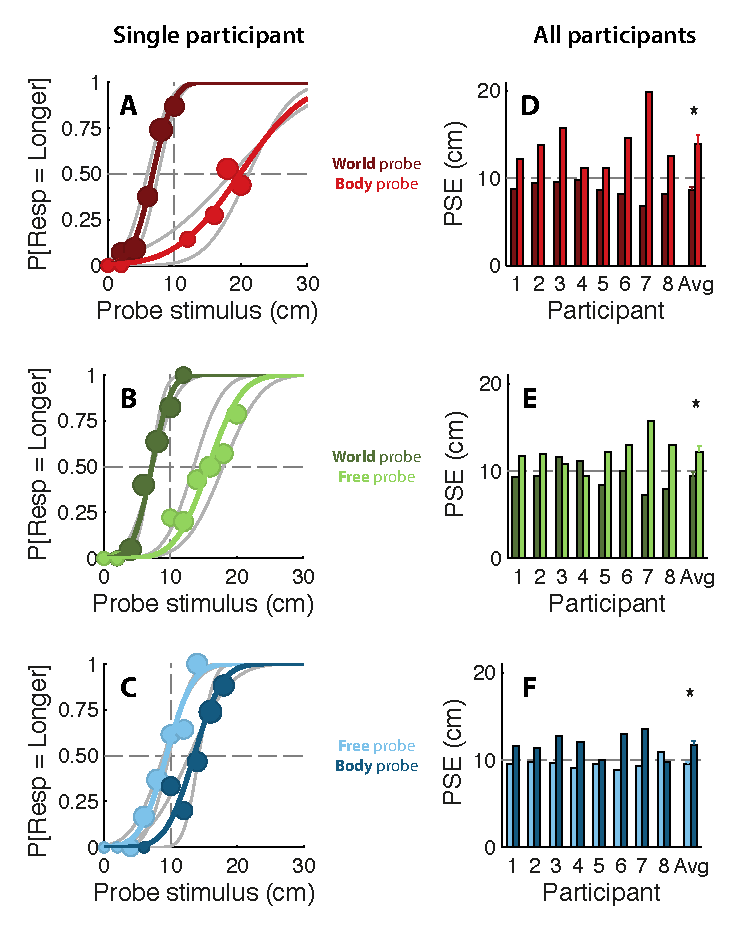
\includegraphics[width=1.0\textwidth]{src/paper3/figure2.pdf}

    \caption{Psychometric curves (colored lines) and associated binned data (circles) for one participant (top row). Circle size represents the number of trials within each 2 \si{\centi\metre} bin. Binning was only done in order to visualize this participant's responses and was not used otherwise. Gray lines show psychometric curves before collapsing across reference order. \panelref{A} Body-world comparison; body reference, dark red; world reference, light red. \panelref{B} World-free comparison; world reference, light green; free reference, dark green. \panelref{C}  Body-free comparison; body reference, dark blue; free reference, light blue. \newline
PSEs for all participants and the average {\textpm}SE (bottom row). \panelref{D} Body-world (dark red) and world-body (light red) conditions. \panelref{E} World-free (light green) and free-world (dark green) conditions. \panelref{F} Body-free (dark blue) and free-body (light blue) conditions. Because a t-test revealed a main effect of reference order, \ttest{47}{-5.2}{0.01}, we used the mean PSE across reference order (e.g. \figref{p3:fig3}, gray lines) instead of the PSE collapsing across reference order (e.g. \figref{p3:fig3}, colored lines); these values were not significantly different.}
    \label{p3:fig2}
\end{figure}

The performance of one participant is illustrated in the left column of \figref{p3:fig2}. Each row shows one main condition: body versus world fixation (top/red), world versus free fixation (middle/green), and body versus free fixation (bottom/blue). The lighter and darker colors in each panel indicate which fixation type was the reference movement (see Legend). The shift of the psychometric functions relative to the 10 \si{\centi\metre} reference (i.e. the PSE) quantifies the influence of fixation type. For example, the rightward shift of the light red curve in \figref{p3:fig2}A means that for a body fixation a longer translation (\about 19 \si{\centi\metre}) was required for that translation to be perceived equivalent to a 10\si{\centi\metre} reference translation with world fixation. On the other hand, the leftward shift of the dark red curve means that a shorter translation with world fixation (\about 7 \si{\centi\metre}) was required for that translation to be perceived equivalent to the 10 \si{\centi\metre} reference translation with body fixation. Together, these oppositely directed shifts demonstrate that translations with world fixation were perceived longer than equivalent translations with body fixation, regardless of which translation was the reference.  Similarly, the shifts in \figref{p3:fig2}B shows that world fixation translations were also perceived to be longer than free fixation movements and \figref{p3:fig2}C shows that free fixation translations were perceived to be longer than body fixation translations. Note that Figure 2 also shows an effects on slope, which will be further discussed in the paragraph \nameref{p3:sec:precision}.

Similar results were obtained for all subjects, as shown by the individual PSEs for all participants (right column of \figref{p3:fig2}). Statistical significance of the fixation-induced effects for each main condition (world versus body, \figref{p3:fig2}D; world versus free, \figref{p3:fig2}E; and free versus body, \figref{p3:fig2}F) was evaluated by comparing PSEs between the two reference conditions using a paired t-test. These PSEs were significantly different in all cases (world versus body, \ttest{7}{-4.09}{0.05}; world versus free, \ttest{7}{-2.48}{0.05}; free versus body, \ttest{7}{-3.38}{0.05}. As for the example subject, these results indicate that translations made with body fixation are perceived shorter than with world fixation, suggesting that self-motion perception is modulated by eye movements even in absence of full-field optic flow. The free fixation translations, which controlling for confounds of the small the fixation point, were perceived to be longer than body and shorter than world fixation translation intervals, which could be expected if their gain would be smaller than 1 but larger than 0.

\begin{figure}
    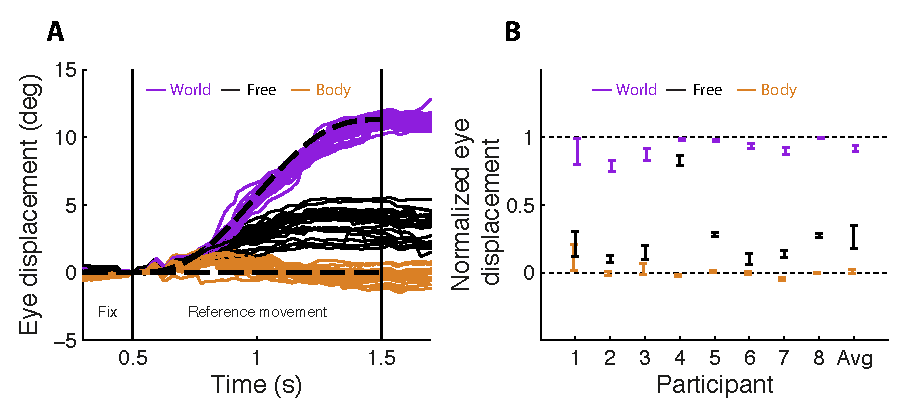
\includegraphics[width=1.0\textwidth]{src/paper3/figure3.pdf}

    \caption{\panelref{A} Actual (solid lines) and ideal (dashed lines) eye movement traces of one participant during world fixation (purple), body fixation (brown), and free fixation (black). All traces shown are for 10 \si{\centi\metre} reference movements. \panelref{B} Normalized eye position for each participant (\textpm95\% confidence interval) at the end of translation interval (error bars) for world fixation (purple), body fixation (brown) and free fixation (blue). In addition, the average {\textpm}SE across all participants is shown. Zero indicates that the eyes remained stationary relative to the body, and one indicates that eye position was perfectly world-fixed.}
    \label{p3:fig3}
\end{figure}

\subsection{Eye movement contributions to self-motion perception}

In order to relate psychophysical performance to eye movement behavior we recorded and analyzed eye movements during both intervals of every trial for all subjects. Exemplar eye traces for the 10 \si{\centi\metre} reference translation for the three fixation types are depicted in \figref{p3:fig3}A. Fixation behavior was quite accurate for both body fixations, where no eye movements were expected, and world fixation, where eye movement excursions of \siang{11} were expected, seemingly supported by  catch-up saccades. Under free fixation, the amount of eye movement was intermediate between body and world fixation and behavior was more variable. A similar pattern was observed in all participants, as illustrated by the normalized eye movement data (see \nameref{p3:sec:methods}, and \figref{p3:fig3}B).

\begin{figure}
    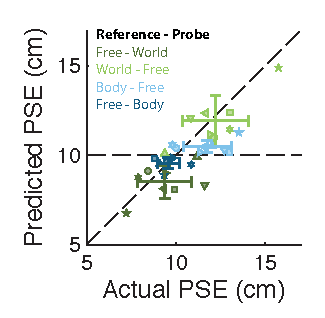
\includegraphics[width=0.5\textwidth]{src/paper3/figure4.pdf}

    \caption{Eye movement based prediction for the PSE plotted against the actual PSE.  A data point (symbol) is shown for each participant (symbol shape) and condition (symbol color) pair, following the same color scheme as in \figref{p3:fig2}. The identity line, corresponding to a perfect prediction, is shown in black.}
    \label{p3:fig4}
\end{figure}

\begin{table}
    \begin{tabular}{llll}
    Participant & Parameter ($\alpha$) \textpm SD \\
    \hline
    1 & 0.27 (\textpm 0.04) \\
    2 & 0.27 (\textpm 0.05) \\
    3 & 0.35 (\textpm 0.04) \\
    4 & 0.06 (\textpm 0.04) \\
    5 & 0.13 (\textpm 0.03) \\
    6 & 0.33 (\textpm 0.04) \\
    7 & 0.58 (\textpm 0.02) \\
    8 & 0.21 (\textpm 0.02) \\    
    \end{tabular}
    
    \caption{Estimated eye movement contribution (α) to the perception of self-motion (see Equation 5). Standard deviations are based on a bootstrap for each participant.}
    
    \label{p3:tab2}
\end{table}

To quantify the role of eye movements in self-motion, we tested a linear model in which perceived translation is a weighted average of a vestibular estimate (equal to the actual translation) and an oculomotor estimate (equal to the normalized eye movement times the actual translation; \eqnref{p3:eq2}). This model contains a single free parameter ($\alpha$), which corresponds to the relative weight given to the oculomotor estimate. We fitted this model to the two body versus world conditions and obtained the value of the oculomotor weight for every subject (\tabref{p3:tab2}). The average oculomotor weight is 0.25 \textpm0.12 (SD), indicating that the contribution of the eye movement signal to the self-motion estimate is about 25 percent. Note that participant 4, whose oculomotor weight is furthest from this mean ($\alpha = 0.06$), also shows a radically different eye movement gain during the free-fixation (see \figref{p3:fig3}B). We then used these oculomotor weights along with the normalized eye movement values to predict the PSEs in the remaining four conditions according to \eqnref{p3:eq5}. The predicted PSEs are plotted against the actually observed PSEs in \figref{p3:fig4}. The positive correlation ($\rho = 0.78$, $p < 0.01$) between observed and predicted PSEs suggests that eye movements are indeed used in self-motion perception, even in the absence of a fixation point (i.e. during free fixation). Furthermore, the fact that data points generally cluster near the unity line shows that our simple model does reasonably well in predicting perceptual performance across subjects and conditions based on oculomotor weight and normalized eye movement magnitude only. This holds true even for subject 7 whose oculomotor weight (\tabref{p3:tab2}) was approximately double the average, yet whose data points remain close to the unity line.

\begin{figure}
    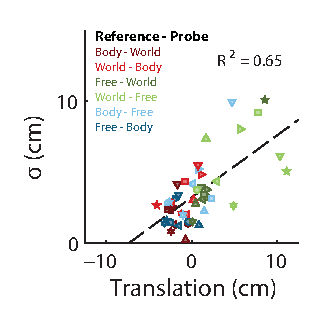
\includegraphics[width=0.5\textwidth]{src/paper3/figure5.pdf}

    \caption{Effect of difference movement amplitude between reference and probe interval (i.e. the bias) on response uncertainty ($\sigma$). A data point is shown for every participant and condition (symbol color) pair, following the same color scheme as in \figref{p3:fig2}. The dashed black line is the linear regression trend line.}
    
    \label{p3:fig5}
\end{figure}

\subsection{Precision depends on the PSE}
\label{p3:sec:precision}

The psychometric curves of the example participant in \figref{p3:fig2} show that precision ($\sigma^{-2}$ in \eqnref{p3:eq1}) decreases as the difference between translated distance in the reference and probe intervals (i.e. the bias) increases. To further investigate this effect, \figref{p3:fig5} shows a linear relation ($R^2 = 0.64$) between the bias and precision across all participants and conditions. This effect, which follows Weber’s perceptual law \cite{fechner1860} is consistent with the signal-dependence of (discrimination) precision that has been shown recently for vertical self-motion \cite{nesti2014}.


\section{Discussion}

We investigated the contribution of eye movements to the perception of passively-induced self-motion. Experiments were performed in the absence of full-field optic flow to eliminate the contribution of this visual motion signal. Perception of self-motion was compared across three fixation types: during free fixation the fixation target was extinguished before the movement, while during world and body fixation, targets  remained stable relative to the world and body, respectively. Our results show that self-motion is underestimated during body fixation (in which the eyes remain stationary) compared to world fixation (in which the eyes move to maintain fixation).The eye movements during free fixation, which  are driven by the VOR, show a non-unity gain with excursions in-between body- and world-fixation conditions. Self-motion perception reflects this pattern of eye movements, suggesting an important contribution of this extraretinal signal to the perception of self-motion.

 To quantitatively characterize the separate vestibular and eye movement contributions, we fit a single parameter model to the perceptual responses for the body versus world comparison conditions and validated this model independently by predicting the effects of eye movements on self-motion perception during free fixation conditions. This model takes into account subject specific oculomotor weight and eye movement patterns. Based on these inputs it accurately predicts the responses in the free fixation conditions. This demonstrates that extra-retinal eye movement signals are used as a cue in the perception of self-motion, contributing significantly to the self-motion percept with a weight of approximately 25 percent, even in the absence of optic flow.
 
It is surprising that an influence of eye movements can be observed even for body- stationary fixations, during which the stationary eye movement signal is clearly in conflict with the non-zero vestibular signal. While this demonstrates the strength of the assumption that fixation targets are world-stationary, it raises the question how reliable this assumption is. Simultaneous recording of angular head and eye movements during natural behavior reveals that approximately 80 percent of eye movements can be classified as compensatory, i.e. eye movements directed opposite to head movement and therefore consistent with maintenance of world-fixed fixation \cite{einhauser2007}. Similarly, other studies have shown that world-stationary fixations are common for many every day activities, ranging from making a cup of tea \cite{hayhoe2014} to driving a car \cite{land1994}, to walking \cite{foulsham2011} and even reaching, where people tend to look at the source and destination of the object, but not at the hand \cite{flanagan2003}. Because world-stationary fixations are so common, the natural world statistics imply that self-motion and eye movements are highly correlated, thus making eye movements a fairly reliable cue for self-motion.

Even when fixation is not world-fixed, eye movement signals are combined with optic flow signals to yield realistic self-motion estimates \cite<e.g>{royden1992, vandenberg2000}. During world-fixed fixation, the eyes move to compensate for body translation, thereby reducing the optic flow component in the retinal signal. The self-motion estimate will therefore be driven predominantly by the eye movement signal. On the other hand, in the body-fixed condition, eye movements are minimal and optic flow maximal such that perceived self-motion will be driven predominantly by the optic flow signal itself. Because our experiment was performed in darkness, this optic flow signal was absent in the body-fixed condition which can explain why self-motion was underestimated.

During body and world fixation, eye movements are driven by retinal slip of the fixation target. However, in the free fixation condition, retinal slip is not available and resulting eye movements resemble the linear vestibulo-ocular reflex (LVOR), in that the gain relative to world fixation was \about0.4 (see \figref{p3:fig3}B; \citeNP{ramat2003}). This reflex is thought to be driven by a double integration of the vestibular signal, converting the head acceleration signal from the otoliths to eye position \cite{green2007,walker2010}. If eye movements during free fixation are in fact vestibularly driven, then combination of this eye movement signal with the vestibular signal itself seems redundant. However such combination could reflect a strategy to reduce noise. Both the direct (vestibular) and indirect (LVOR) signals depend on integration of the linear acceleration signal and may be corrupted by independent noise sources. Combining them in a statistically optimal fashion will decrease the noise level towards the noise level of the original source signal \cite{faisal2008,clemens2011,fetsch2013}. The consequence of this integration will be a reduced self-motion estimate when the gain of the LVOR is less than 1, as we observed in the free condition.

\subsection{Alternative interpretations}

In the above, we suggest that eye movements themselves drive perception of self-motion. However, it is conceivable that a common correlate of eye movements, such as attention or visual motion influenced our results. In 1963, Guedry and Harris reported a substantial underestimation of displacement when their observers watched a small body-fixed target compared to displacements in the dark. They attributed their findings to an attentional shift from judgements of body displacement in the dark to judgements of target displacement in the fixation condition. We favor an explanation based on eye movement characteristics.  In their study, it is likely that the VOR caused eye movements  to occur during the translations in darkness. If these movements were used to augment self-motion perception, then the perception of such translations would be overestimated compared to translations made without eye movements, e.g. when fixating a body-fixed target. Because Guedry and Harris \citeyear{guedry1963} did neither record nor explicitly manipulate eye movements, they were not able to unveil their explicit role. Conversely, we did not manipulate attentional processes \cite{kitazaki2003}, so we cannot completely exclude the possibility they play a role.

Others have reported errors in the disambiguation of self and object-motion. Examples include the perceived motion of body-fixed visual targets during angular acceleration (the oculogyral illusion; \citeNP{carriot2011}), the apparent displacement of body-fixed stimuli during linear acceleration (the oculogravic illusion; \citeNP{graybiel1952}) and the apparent movement of world-stationary targets during self-motion in darkness \cite{dyde2008}. Similar disambiguation errors could cause the effects we observed. More specifically, if movement of the fixation point relative to the observer were always attributed to self-motion, then self-motion would be underestimated during body relative to world fixation, as we observed. However, such attribution errors cannot account for the effects in the free condition, because no fixation point was visible and no attribution was required. In the free condition, we demonstrate that eye movements by themselves, occurring in the absence of visual tracking and other external cues, influence the perception of self-motion.

\subsection{Implications for other studies}

Many previous self-motion studies have used a body-fixed fixation point to control for eye movement related effects. Our results suggest, however, that using a body-fixed fixation point causes underestimation of self-motion. For example, Li, Wei, and Angelaki \citeyear{li2005a} investigated spatial updating across lateral translation and found that saccades to updated targets undershot the actual target location. As self-motion perception drives this update, the effects of eye movements on self-motion perception should also influence the updating process. In other words, the observed undershoot could be due to the underestimation of self-motion caused by the body-fixed fixation point. Another example is a study on the perception of vertical object-motion during lateral translation \cite{dokka2013}. This study reports incomplete compensation for self-motion when judging the deviation from vertical motion of a moving object. This observation could also be due to underestimation of self-motion induced by the fixation of the body-fixed target.

A moving fixation point is also known to influence self-motion perception, as in the Slalom Illusion \cite{freeman2000}; observers viewing expanding optic flow while fixating a target that oscillates from left to right perceive slaloming motion which is inconsistent with the purely forward motion specified by the expanding optic flow display. However, this observation is consistent with the idea that oculomotor signals are used in estimating self-motion. Additionally, it has been shown that eye movements affect postural sway \cite{glasauer2005}.  Participants performed smooth pursuit eye movements in complete darkness and displayed lateral sway consistent with the stabilization of posture using a self-motion estimate influenced by pursuit eye movements.

Studies conducted to characterize vestibular-only sensitivity are often performed in complete darkness or with closed eyes \cite{grabherr2008,  macneilage2010b, macneilage2010a, roditi2012, valko2012, nesti2014}. However, the results of our free-fixation condition suggest that even under these circumstances, results could easily be influenced by vestibularly driven eye movements. Overall, we suggest that any study concerned with self-motion processing must consider the possible influence of eye movements.

\subsection{Possible neural substrate}

This leaves us with the question of where in the brain these effects originate. The locus of our effect is likely to carry both eye movement and vestibular signals. Prime candidate areas known to carry both vestibular and eye movement signals are the vestibular nuclei \cite{henn1974,daunton1979} and the cerebellum \cite{waespe1981}. On the other hand, eye movements could influence self-motion perception indirectly via optic flow processing. In particular, cortical areas that carry both vestibular and optic flow signals (which can be modulated by eye movements) include the ventral intraparietal area (VIP; \citeNP{bremmer2002,chen2011}), and the dorsal medial superior temporal area (MSTd; \citeNP{gu2008}). Future work should reveal how such brain areas, directly or indirectly, merge both vestibular and oculomotor signals into a coherent percept of self-motion.



\bibliography{refs}{}

\titleformat{\chapter}
{\normalfont\Large\bfseries}{\thechapter}{0.2em}{}
\titlespacing*{\chapter}{0pt}{-30pt}{10pt}

\end{document}

\documentclass[10pt,b5paper,twoside]{book}


%
% Common packages and custom commands used by the main .tex files.
%

\usepackage[dutch,british]{babel}
\usepackage[nottoc]{tocbibind}
\usepackage{amsmath}
\usepackage{amsfonts}
\usepackage{amssymb}
\usepackage{graphicx}
\usepackage{gensymb}
\usepackage{textcomp}
\usepackage{hyperref}
\usepackage{doi}
\usepackage{xcolor}
\usepackage{nameref}
\usepackage{xspace}
\usepackage{titlesec}
\usepackage{floatrow}
\usepackage{longtable}
\usepackage{siunitx}
\usepackage[outercaption]{sidecap}
%\usepackage{fancyhdr}
\usepackage{wrapfig}
\usepackage{lmodern}
\usepackage[font={scriptsize, sf}, labelfont={sf,scriptsize,bf}]{caption}
\usepackage{src/apacite_custom}
\usepackage{src/thesis}

\pagestyle{plain}

\floatsetup[table]{font={scriptsize, sf}}

\hypersetup{colorlinks=true, linkcolor=blue, citecolor=blue}
\setcounter{tocdepth}{2}

% Do not add extra vertical space
\raggedbottom

% Indent paragraphs
\setlength{\parindent}{1.0cm}

\bibliographystyle{apacite_custom}

\renewcommand{\baselinestretch}{1.2}
\setlength{\parskip}{0ex plus 0.3ex minus 0.3ex}

\newcommand{\about}{$\approx$}

%% For the Chapter title, etc.
\newcommand{\bigrule}{\titlerule[0.5mm]}
\titleformat{\chapter}[display]
{\normalfont\filleft\bfseries\itshape}
{%
 \vskip-3em
\titlerule[1pt]%
\vspace{1pt}%
\titlerule
\vspace{1pc}%
\Large\MakeUppercase{\chaptertitlename} \thechapter}
{1pc}
{\titlerule
\vspace{1pc}%
\thispagestyle{empty}
\Huge}


\hypersetup{
    pdfauthor = {Ivar Clemens},
    %pdftitle = {Choosing our words},
    %pdfsubject = {Language production},
    %pdfkeywords = {language production; }
}

\begin{document}

\selectlanguage{british}

\chapter{Translation perception is modulated by eye movements that are partially scaled by fixation depth}
\chaptermark{}

\label{p4}

\newpage

\small {\bf Abstract}
It has been shown that the compensatory eye movements, that minimise retinal slip during self-motion, also serve as a cue for translation perception. However, to provide an adequate translation estimate, the brain must internally scale these ensuing eye movements by fixation distance. Using a 2AFC approach, we investigated whether the brain applies this scaling.  Participants ($n = 8$) were translated sideways in the absence of full-field optic flow but with gaze maintained on either a nearby or faraway target, that was either fixed in the world (world-fixed) or moved along with the body (body-fixed). Results show that translations were perceived shorter with gaze on nearby than faraway world-fixed targets, indicating that eye movements are not properly scaled in translation perception. Translation perception was not affected by the depth of body-fixed targets. Taken together, our results suggest that eye movements are merely a rudimentary cue to self-motion, with a compensation for fixation depth that is partial at best.

\vfill

\noindent\underline{ \hspace{4cm} }

\noindent This chapter is being prepared for publication \newline
\noindent {\bf Clemens, I.A.H.}, Selen, L.P.J., MacNeilage, P.R. and Medendorp, W.P. \citeyear{clemens2015b}. %Title. \emph{Journal}, volume(issue): from-to. \newline

\newpage


%%%%%%%%%%%%%%%%
% Introduction %
%%%%%%%%%%%%%%%%


\section{Introduction}

An accurate internal estimate of self-motion is required to navigate effectively through a complex three-dimensional environment. The vestibular system as well as optic flow provide essential information about self-motion \cite{gibson1955, benson1986, harris2000, israel1989, angelaki2005, carriot2013, chen2010}. During navigation, however, the eyes typically move to maintain visual acuity on important objects. These eye movements disturb the optic flow patterns. Using the oculomotor signal, the brain is able to account for these disturbances by internally separating optic flow into two components, one caused by self-motion and the other by eye movement \cite{warren1988, royden1992, freeman1998, lappe1999}.

When the eyes track world-centred objects, their angular displacement is directly related to the size of the motion of the observer \cite{schwarz1989, paige1998, mchenry2000, medendorp2002}. Because  the majority of fixations are on world-stationary  objects, we recently proposed that these tracking eye movements could also be used as a self-motion cue, in addition to optic flow and vestibular signals. To test this hypothesis, we compared self-motion perception in the absence of full-field optic flow during passively induced whole-body translations \cite{clemens2015a}. Our results showed that self-motion is underestimated during body-centred fixations (in which the eyes remain stationary in their orbits) compared to fixations on world-stationary objects (in which the eyes must move to maintain fixation).

Geometrically, eye movements that keep fixation on a world-centred target during lateral whole body translation (i.e. the linear vestibulo-ocular reflex; LVOR), must scale with fixation depth \cite{angelaki2004}. When fixating body-centred targets these eye movements must be suppressed irrespective of fixation distance \cite{angelaki2004}. Conversely, when fixating world-centred targets, the brain must internally scale the ensuing eye movement by fixation distance to serve as an adequate self-motion cue. Because we did not manipulate fixation distance in our previous study, we could not dissociate whether eye movements are used as a rudimentary cue for self-motion (i.e. without taking fixation depth into account), or are properly scaled in the mechanisms for self-motion perception.

In the present study, we investigate how fixation distance influences perception of self-motion during passive side-to-side translations. Using a psychophysical approach, participants had to indicate whether the second body displacement of two one-second translation intervals was smaller or longer than the first. We show that translation amplitude is perceived smaller when fixating a far compared to a nearby world-centred target, indicating that eye movements are not properly scaled in self-motion perception. Together with the observation that self-motion perception is not affected by the depth of a body-centred fixation target, we conclude that eye movements are merely a rudimentary cue to self-motion, with a compensation for fixation depth that is partial at best.


%%%%%%%%%%%
% Methods %
%%%%%%%%%%%


\section{Materials and methods}
\label{p4:sec:methods}

\subsection{Participants}

Eight naive participants (three male, five female), aged between 22 and 29 years, gave written informed consent to participate in the study. They were all free of any known vestibular or neurological disorder and had normal or corrected-to-normal visual acuity. Participants never received any feedback about their performance.  The experimental setup and methods used here are similar to those used in our previous paper on the influence of eye movement type on self-motion perception \cite{clemens2015a}. We only provide a brief summary here, and refer to our previous paper for further details.

\subsection{Experimental setup}

Participants were seated on a motorised linear sled with their body and head restrained such that the inter-aural axis aligned with the motion axis. The sled laterally translated participants following a minimum jerk profile of fixed duration (1 \si{\second}) and amplitudes ranging from 1 to 27 \si{\centi\metre}. Auditory cues were suppressed using white noise presented through in-ear head-phones. Experiments were conducted in complete darkness except for visual fixation points, projected by body- or world-fixed laser pointers on a black bar, either 50 or 200 \si{\centi\metre} in front of the participant and at eye level. Eye movements were recorded at 500Hz using an EyeLink II system (SR Research, Kanata, Canada). Eye position was calibrated before every session using 11 evenly spaced calibration points ranging from -22 to 22 degrees.


\subsection{Paradigm}

We used a two-alternative forced choice (2AFC) task to study the influence of fixation depth on the perception of linear translation. We tested two fixation depths: near (50 \si{\centi\metre}) and far (200 \si{\centi\metre}) and two different eye fixation conditions: world-, and body-fixed fixation. A trial contained two sequential motion intervals of equal duration (1 \si{\second}), with the motion in the same direction (either leftward or rightward).

%Fixation condition (world-, or body-fixed) was the same in both intervals, but a different fixation depth was presented in each. Participants had to judge whether the translation during the second motion interval was longer or shorter than in the first motion interval.

\begin{figure}
    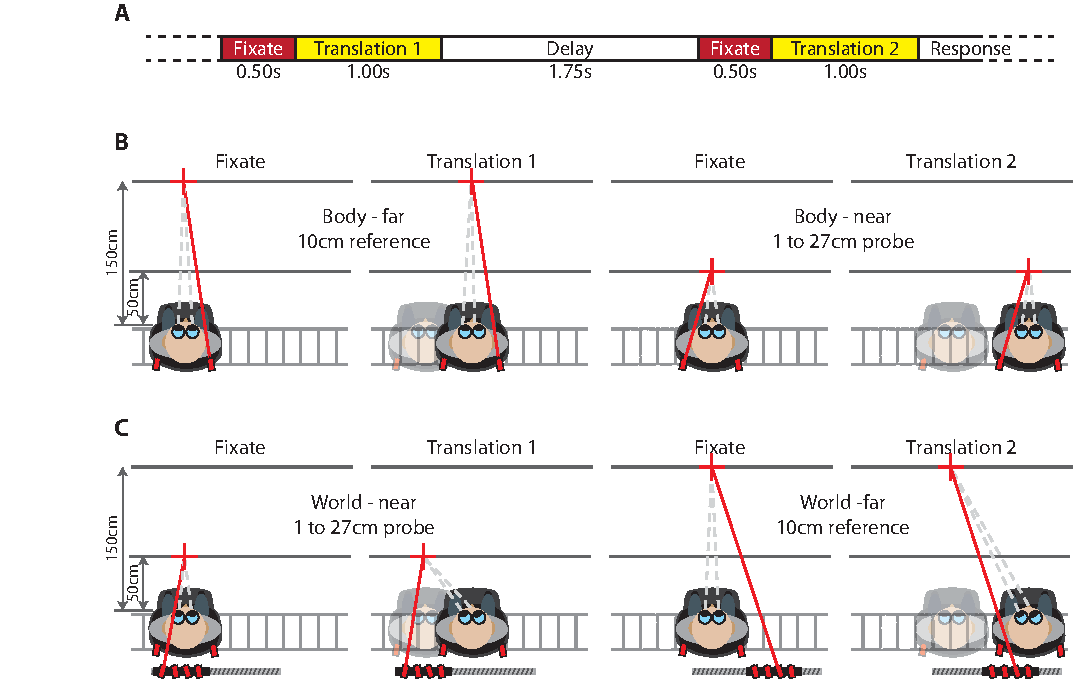
\includegraphics[width=1.0\textwidth]{src/paper4/p4_figure1.pdf}

    \caption{\panel{A} Time course  of key events within a single trial. In each of the two intervals, a 0.50 \si{\second} fixation period (red) precedes the lateral translation (yellow). A 1.75 \si{\second} long delay period (shown in white) separates the two intervals. After the second translation, the participant responded whether this second translation was longer or shorter than the first. \panel{B} and \panel{C} Top-view illustrating key events in a far versus near body-fixed fixation trial (\panel{B}) and a near versus far world-fixed fixation trial (\panel{C}). The first panel shows the initial fixation to the target (red cross) followed by a translation in the second panel. The third panel shows the initial fixation before the second movement interval followed by a translation in the fourth panel.}
    \label{p4:fig1}
\end{figure}

The timing of a single trial is shown in \panelref{p4:fig1}{A}. Every trial started with the onset of a central fixation point (i.e. aligned between the eyes), at a depth of 50 or 200\si{\centi\metre}, for 0.5 \si{\second}. Subsequently, the first 1\si{\second} motion interval commenced. During this translation, the fixation point either remained world stationary (world condition), or moved along with the participant (body condition).  Subsequently a 1.75 \si{\second} delay followed in which the sled was stationary and no  fixation light was shown. Next, a central fixation point reappeared at the other depth (50 or 200\si{\centi\metre}) than was used in the first interval. After 0.5 \si{\second}, the second 1 \si{\second} translation interval started, with the same fixation condition as in the first interval. After this second interval, the participant responded whether the second displacement was perceived longer or shorter than the first by moving a 1-dimensional joystick away from (longer) or towards (shorter) the body. Top-view illustrations of example body-centred and world-centred trials are shown in \panelref{p4:fig1}{B} and \hyperref[p4:fig1]{C} respectively.

\begin{table}
    \begin{tabular}{llll}
    Comparison & Reference & 1st interval & Direction \\
    \hline
    Body & Near & Reference & Right \\
    Near vs. far & & & Left \\
    & & Probe & Right \\
    & & & Left \\
    \cline{2-4}
	& Far & Reference & Right \\
    & & & Left \\
    & & Probe & Right \\
    & & & Left \\
    \hline
    World & Near & Reference & Right \\
    Near vs. far & & & Left \\
    & & Probe & Right \\
    & & & Left \\
    \cline{2-4}
	& Far & Reference & Right \\
    & & & Left \\
    & & Probe & Right \\
    & & & Left \\
    \end{tabular}

    \caption{List of the 2 main comparisons that we tested. The (10cm) reference movement was presented in either the first or the second interval. We also manipulated movement direction (leftward vs rightward) yielding a total of 16 trial types.}

    \label{p4:tab1}
\end{table}

% Should look at the 4 vs 16 in the next part, sounds confusing.
Across trials, we varied the order of the fixation depths and the order  of the reference and probe interval, resulting in four variations of both the world and body condition (see \tabref{p4:tab1}).

Leftward and rightward motion alternated between trials, but were not considered as variations of the condition. To determine the point of subjective quality (PSE), the size of the probe translation was adaptively chosen based on the participants' earlier responses (Psi method; \citeNP{kontsevich1999}). This was done separately for all 16 trial types (2 main conditions x 2 depth orders x 2 reference/probe orders x 2 movement directions; see Table 1). A total of 25 trials was collected per trial type yielding a total of 200 trials for each of the two main conditions.

These trials were presented in two one-hour sessions. To prevent dark adaptation, we turned on the lights for 5 \si{\second} after every 8 trials, and for at least 30 s after every 16 trials. Each of the 16 unique trial types were presented once in every block of 16 trials. After each block, the adaptive procedure determined which translation size to test in the following block. To increase the number of data-points available to the adaptive psychometric procedure at the beginning of the experiment, we collapsed across movement direction and reference order for the first 10 trials. After that, the procedure ran separately for the 16 distinct trial types.

\subsection{Data analysis}

For each combination of the two main conditions and the two reference/probe orders we computed the probability $P(x)$ of probe translation $x$ being  judged as longer than the reference translation. To summarise these data, we fit cumulative Gaussian functions to these probabilities, resulting in a total of four Gaussian functions per participant (see \tabref{p4:tab1}):

\begin{equation}
\label{p4:eq1}
P(x) = \lambda + (1 - 2\lambda) \frac{1}{\sigma \sqrt{2\pi}} \int_{-\infty}^{x}{e^{-(y-\mu)^2 / 2\sigma^2}}dy,
\end{equation}

The mean of the Gaussian, $\mu$, represents the point of subjective equality (PSE). The slope of the curve reflects the precision ($1/\sigma$) of reference-probe discrimination performance. Parameter $\lambda$, representing the lapse rate, accounts for stimulus-independent errors caused by subject lapses or mistakes and was restricted to small values ($\lambda < 0.06$). Fits were performed using the Psignifit toolbox \cite{wichmann2001,wichmann2001b}.

For each trial type (see \tabref{p4:tab1}), we also quantified the eye movements, corrected for drift based on initial fixation. We discarded trials containing blinks as well as trials in which final eye position exceeded two standard deviations from the condition's average. Based on these criteria, 12\% of all trials were discarded. Of the remaining trials, we computed the average ratio between the measured eye excursion, $\varphi_i$, and the angle that  the eyes would have  moved through had they perfectly tracked a world-stationary fixation target at the same fixation depth. The latter is computed by taking the arc-tangent of the actual translation distance, $m_i$, divided by the fixation depth, $d_i$, which for small $\varphi$ can be approximated by $g_c = \frac{\varphi_i m_i}{d_i}$. We computed this ratio, $g_c$, for every trial type $c$ (see \tabref{p4:tab1}). Ideally, for body-fixed trials, $g_c = 0$; and for world-fixed trials, $g_c = 1$.


\subsection{Model}

Using a straightforward model, we investigate to what extent fixation depth is taken into account in the contribution of eye movements to self-motion perception. As in \citeA{clemens2015a}, we model the perceived translation, $p_i$, as a weighted combination of a vestibular, $m_i$, and oculomotor estimate of translation, $\hat{\varphi}_i$ (\eqnref{p4:eq4}).

\begin{equation}
\label{p4:eq4}
p_i = \alpha_{d_i} \hat{\varphi}_i + (1 - \alpha_{d_i}) m_i
\end{equation}

Variable $i$ represents either the reference, $r$, or probe, $p$, interval. To serve as a veridical cue for self-motion, eye movements need to be scaled by the depth of fixation, $d$. This scaling is reflected by parameter, $\alpha_{d_i}$. If this parameter is the same across the two fixation depths, $d$, then there is no depth-dependent modulation of the oculomotor estimate of translation.

By definition, at the PSE, the probe translation is perceived as equal in length to the 10 cm reference translation, $p_r = p_p$. By substituting both sides by the right hand side of \eqnref{p4:eq4}, we obtain:

\begin{equation}
\label{p4:eq5}
\alpha_{d_r} \hat{\varphi}_r + (1 - \alpha_{d_r}) m_r = \alpha_{d_p} \hat{\varphi}_p + (1 - \alpha_{d_p}) m_p + \epsilon
\end{equation}

We fit \eqnref{p4:eq5} to the data using linear regression, finding one weight for each of the two fixation depths (that is, $\alpha_{50}$ and $\alpha_{200}$) that minimises the sum of squared errors ($\Sigma \epsilon^2$). Because these parameters can, in theory, contain both a depth-dependent and a depth-independent scaling, we compute their ratio, $\alpha_{200}/\alpha_{50}$, to remove any depth independent components. In case of perfect compensation, the expected ratio is $200/50 = 4$, while in case of depth-independent scaling it is 1.


%%%%%%%%%%%
% Results %
%%%%%%%%%%%


\section{Results}

In a recent study we have shown that eye movement signals contribute to the perception of body translation, even in the absence of optic flow or a visual fixation point \cite{clemens2015a}. Because eye rotations must be scaled by target depth ($\varphi d = T$) to serve as an adequate translation cue, we tested self-motion perception for near (50 \si{\centi\metre}) and far (200 \si{\centi\metre}) fixations. Participants were presented with two subsequent translations \figref{p4:fig1} while they kept fixation on a world- or body-stationary target that was presented either nearby or far away. After the two translation intervals, participants had to judge whether the second translation was longer or shorter than the first.

\begin{figure}
    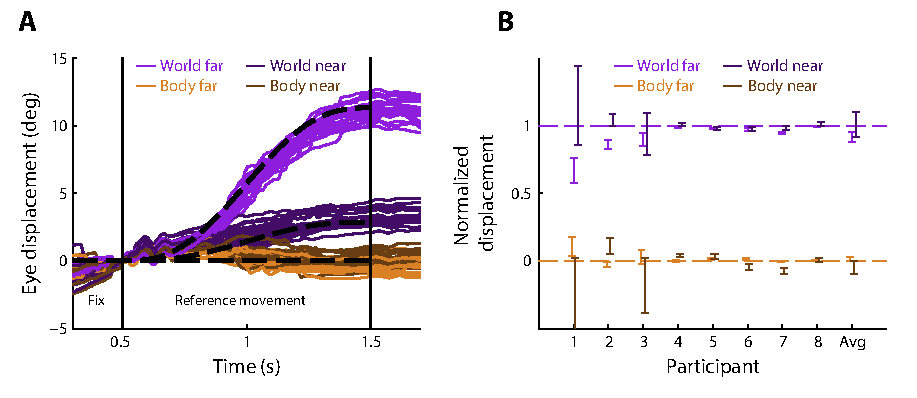
\includegraphics[width=1.0\textwidth]{src/paper4/p4_figure2.pdf}

    \caption{\panel{A} Actual (solid lines) and ideal (dashed lines) eye movement traces of one participant in the body-fixed (brown and orange) and world-fixed conditions (purple and pink). Gaze was directed at a near (brown and purple) or far (orange and pink) target. All traces shown are for 10 \si{\centi\metre} reference displacements. \panel{B} Normalised eye position for each participant (\textpm 95\% confidence interval) at the end of the translation interval for the near and far world fixed targets (purple and pink respectively) as well as the near and far body fixed fixation targets (brown and orange respectively). In addition, the average \textpm SE across all participants is shown. Zero indicates the eyes remained stationary relative to the body, and one indicates the eyes followed the near world fixed target perfectly.}
    \label{p4:fig2}
\end{figure}

We first investigated the ability of participants to fixate body and world stationary targets. \panelref{p4:fig2}{A} depicts exemplar eye traces for the 10cm reference translation with nearby and far fixation points in both the body and world condition. Changes in gaze are largely absent in the body near and body far conditions (brown and orange traces respectively), as required. During the world conditions, the eye excursions were large when fixating nearby targets and small when fixating far away ones (purple and pink traces respectively), which reflects the geometrical constraints.

We normalised the eye movement data by taking the average ratio between the measured eye excursion and the geometrically required eye displacement were the target world stationary. \panelref{p4:fig2}{B} shows that these normalised eye displacements are about zero during body fixed fixations (brown and orange) and close to one in the world fixed fixations (purple and pink data points), for all participants. The question is whether these eye movements are inversely scaled by fixation depth in order to interpret them as linear self-motion cues.

\begin{figure}
    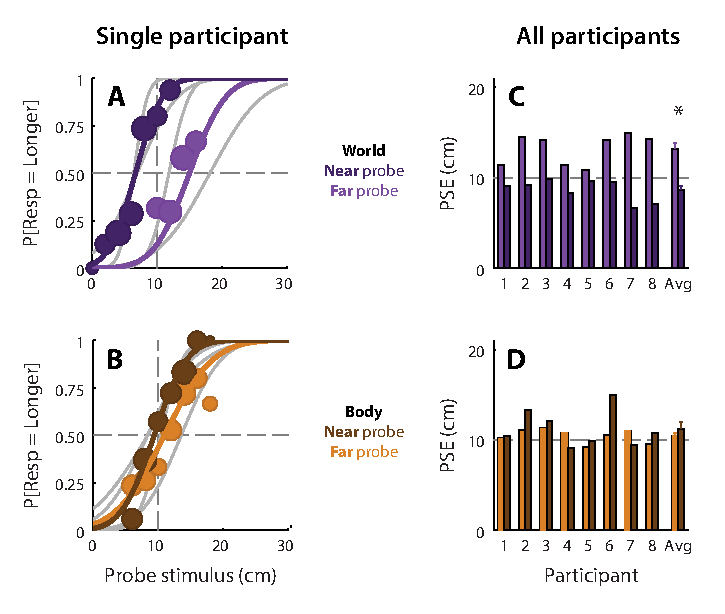
\includegraphics[width=1.0\textwidth]{src/paper4/p4_figure3.pdf}

	\caption{\panel{A} and \panel{B} Psychometric curves (coloured lines) and associated binned data (circles) for one participant. Circle size represents the amount of trials within the bin. Psychometric curves before collapsing across reference order are shown as gray lines. \panel{A} World-fixed condition (purple) while fixation was either near (dark) or far (light). \panel{B} Body-fixed condition (brown) while fixation was either near (dark) or far (light).
	\panel{C} and \panel{D} Individual and average points of subjective equality (PSEs). Colour scheme matches panels A and B.
	}
	\label{p4:fig3}
\end{figure}

\figref{p4:fig3} illustrates psychophysical data on self-motion perception of a single participant for the two-fixation depths in both the world (\panelref{p4:fig3}{A}) and body condition (\panelref{p4:fig3}{B}). Lighter and darker colours indicate which fixation depth was the reference translation (see figure legend). The influence of fixation depth is characterised by a shift of the psychometric functions relative to the 10 \si{\centi\metre} reference translation (i.e. the PSE). For example, the rightward shift of the pink curve in \panelref{p4:fig3}{A}, representing the world-condition, means that with a far target a longer translation (\about15 \si{\centi\metre}) was required to be perceived equivalent to a 10 \si{\centi\metre} reference translation with nearby fixation. Likewise, the leftward shift of the purple curve indicates that a shorter translation with near fixation (\about6 \si{\centi\metre}) is required to be perceived the same as the 10 \si{\centi\metre} reference translation with far fixation. Together, these opposite biases suggest that translations are perceived shorter for fixations further away. For the body condition, no shift of the psychometric curves is visible (\panelref{p4:fig3}{B}), indicating that fixation depth (i.e. near versus far) has no effect in absence of eye movements.

Similar results were obtained for all participants, as shown by the individual PSEs (right column of \figref{p4:fig3}). Statistical significance of the effects of fixation depth was evaluated by comparing PSEs for the two fixation depths using a paired t-test. PSEs  differed significantly between the two fixation depths in the world condition, $t(7) = 5.42$, $p < 0.01$ (\panelref{p4:fig3}{C}), but not in the body condition, $t(7) = -1.17$, $p = 0.28$ (\panelref{p4:fig3}{D}), confirming the single subject results (\panelref{p4:fig3}{A and B}). Thus, increasing fixation depth does not influence self-motion perception during body-stationary fixations, but causes self-motion to be perceived as shorter during world-stationary fixations.

\begin{table}
    \begin{tabular}{l|lll|l}
	Participant & $\alpha_{50}$ & $\alpha_{200}$ & $\frac{d_{200}}{d_{50}}$ & $\alpha$ \\
    \hline
	1 & 0.37 & 0.25 & 1.46 & 0.27 \\
	2 & 0.51 & 0.41 & 1.25 & 0.27 \\
	3 & 0.36 & 0.30 & 1.22 & 0.35 \\
	4 & 0.14 & 0.29 & 0.49 & 0.06 \\
	5 & 0.11 & 0.04 & 2.79 & 0.13 \\
	6 & 0.49 & 0.15 & 3.34 & 0.33\\
	7 & 0.40 & 0.53 & 0.76 & 0.58 \\
	8 & 0.42 & 0.35 & 1.25 & 0.21 \\
    \end{tabular}

    \caption{Best-fit parameter values for 50 and 200 \si{\centi\metre} fixation distances, $\alpha_{50}$ and $\alpha_{200}$ respectively (see \eqnref{p4:eq5}), and their ratio, $\alpha_{200} / \alpha_{50} = d_{200} / d_{50}$, for each participant. Best-fit parameter values, $\alpha$, from our previous paper \protect\cite{clemens2015a} are included for reference.}

    \label{p4:tab2}
\end{table}

\begin{figure}
    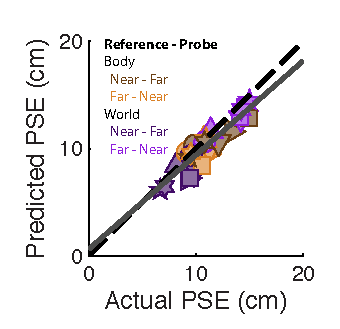
\includegraphics[width=0.5\textwidth]{src/paper4/p4_figure4.pdf}

	\caption{Eye movement based prediction for the PSE plotted against the actual PSE. A data point (symbol) is shown for each participant (symbol shape) and condition (symbol colour) pair, following the same colour scheme as in \figref{p4:fig3}. The identity line, corresponding to a perfect prediction is shown (solid line) as well as the best fit line (dashed).}
	\label{p4:fig4}
\end{figure}

We used a simple linear model to quantify to what extent eye movements are scaled by fixation depth in order to serve as a linear self-motion cue (see \nameref{p4:sec:methods}). This model describes the perceived translation distance as a weighted average of a vestibular estimate, equal to the actual translation, and an oculomotor-based estimate. The latter estimate depends on the eye excursion which should be scaled by fixation depth to serve as a valid cue. Our model contained two weighting parameters, $\alpha_{50}$ and $\alpha_{200}$, one per fixation depth (see \tabref{p4:tab2} for best-fit values). Using these parameters we predicted the PSEs, i.e. $m_p$ in \eqnref{p4:eq5}, and plotted them against the actually observed PSEs in \figref{p4:fig4}. The positive correlation ($\rho = 0.92$, $p < 0.01$) between observed and predicted PSEs shows that our simple model does reasonably well in predicting perceptual performance.

\begin{figure}
    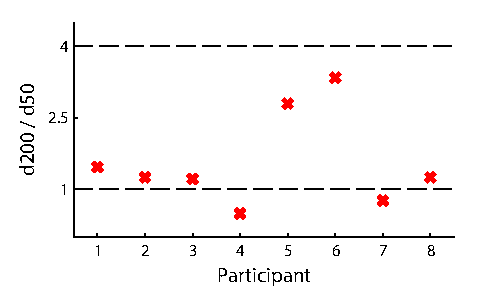
\includegraphics[width=0.75\textwidth]{src/paper4/p4_figure5.pdf}

	\caption{Ratio between near and far parameter values, $\alpha_{200} / \alpha_{50} = d_{200} / d_{50}$ for every participant. Both perfect depth compensation, $\alpha_{200} / \alpha_{50} = 200 / 50 = 4$, as well as the lack thereof, $\alpha_{200} / \alpha{50} = 1$, are represented by a dashed line.}
	\label{p4:fig5}
\end{figure}

By examining the ratio of these weighting parameters, we remove any depth-independent contributions. In absence of  depth scaling, i.e. when $d_{50} = d_{200}$, the ratio should be one. For perfect compensation, that is when $d_{50} = 50  \wedge d_{200} = 200$, the ratio should be $4$. The actual ratio between $d_{50}$ and $d_{200}$ is plotted for each participant in \figref{p4:fig5}. While two participants show moderate compensation for depth, the majority of participants show no clear sign of scaling of eye movements by fixation distance. This is consistent with the observation that translations are perceived shorter with far compared to near fixations in the world condition.


%%%%%%%%%%%%%%
% Discussion %
%%%%%%%%%%%%%%


\section{Discussion}

% Relation to previous work / Should rewrite this paragraph!
In our previous study, we demonstrated that oculomotor signals play a substantial role in the perception of translation, even in the absence of optic flow or any other visual stimulation \cite{clemens2015a}. Although the vestibular system provided the most significant contribution, oculomotor signals were shown to account for about 20\% of the overall percept. Because these experiments were performed with a single fixation depth, it was not clear whether the brain weighted the oculomotor signal in a depth-dependent manner when using it as a translation cue, or merely uses the signal as a rudimentary cue to self-motion. In the present study we tested between these two possibilities.

% Basic observations
We assessed translation perception during both body- and world-fixed fixation at two different fixation depths. Our results show that self-motion was underestimated when comparing far and near fixation trials in the world-fixed condition, which argues against a proper scaling of the eye movement signal. Fixation depth did not influence translation perception during body-fixed fixation (where eye movements are virtually absent).

% Model results
To quantify the relative depth-dependent scaling of eye movements for nearby and far away fixation targets, we fitted a straightforward linear model to the perceptual responses based on the oculomotor behaviour across four conditions. While two participants show partial scaling, the other six participants did not show any sign of scaling. Thus, we conclude that while oculomotor signals provide a robust cue to translation perception, they are not properly scaled by fixation depth.


\subsection{Relation to other studies}

% Relation to Clemens, 2015
\begin{figure}
    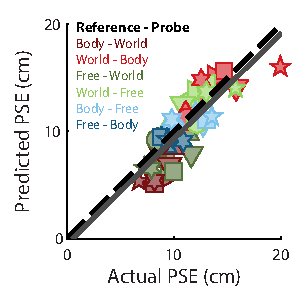
\includegraphics[width=0.5\textwidth]{src/paper4/p4_figure6.pdf}

    \caption{Predicted versus actual PSEs for Clemens \protect\citeyear{clemens2015a} using parameter $\alpha_{50}$ from the present paper. A data point (symbol) is shown for each participant (symbol shape) and condition (symbol colour) pair, following the same colour scheme as in \protect\figref{p3:fig2}: Body-world comparison; body reference, dark red; world reference, light red. World-free comparison; world reference, light green; free reference, dark green. Body-free comparison; body reference, dark blue; free reference, light blue.}
    \label{p4:fig6}
\end{figure}

In our previous experiment we compared translation perception with body-fixed versus world-fixed fixations at near depth (50 \si{\centi\metre}) only \cite{clemens2015a}. \figref{p4:fig6} shows how well our $\alpha_{50}$ parameter explains the data in our previous paper. The positive correlation between the actual PSEs in the previous study and those predicted using the model of the present paper ($\rho = 0.60$, $p = 0.06$) adds confidence to the parameter values presented here. The average difference between the values found here and those reported previously (see \tabref{p4:tab2}) is 12 \textpm 8 percent-points, which is relatively small given the independent measurements.

% Relation to the VOR
The function of the LVOR is to keep the eyes stable in the world during linear translation \cite{paige1989,busettini1994,paige1998}. Because it also needs to scale with fixation depth \cite{angelaki2004}, it is possible that the LVOR and self-motion perception have the same underlying signal. Because of the visual fixation point in our paradigm, visual following mechanisms may even augment the LVOR compensation. If the oculomotor signal generated by the LVOR is used for self-motion perception, one would expect that the LVOR compensation at 50 and 200cm closely relate to the corresponding oculomotor weights in the present study (see \figref{p4:fig5} and \tabref{p4:tab2}). To further explore this, we derived the LVOR gains for 50 and 200 \si{\centi\metre} from Paige et al. \citeyear{paige1989} and computed their expected depth ratio, $d_{200} / d_{50}$. This ratio, 1.87, is in between the ratio of the 6 participants who did not show any sign of scaling ($\frac{d_{200}}{d_{50}} = 1.07 \pm 0.16$) and the 2 participants that did show scaling ($\frac{d_{200}}{d_{50}} = 3.06 \pm 0.27$), suggesting that our effect might share a pathway with the LVOR.


\subsection{Alternative explanations}

It is important to point out that while the vestibular signal and thus noise is constant for a given translation distance, the noise in the associated oculomotor estimate might change with fixation distance because the magnitude of the eye movement is modulated by fixation depth and may show signal-dependent noise.

If this were the case, the nearby world-fixed fixations would cause larger eye movements with more noise compared to the far world-fixed fixations with smaller eye movements. The oculomotor based translation estimate would be weighted less for near versus far fixation, potentially explaining the partial compensation for fixation depth we have observed. In addition, the noise levels in the oculomotor estimate could also depend on fixation depth itself: the retinal displacement of a world stationary fixation point decreases with fixation depth, making it less informative about the amount of self-motion. The noise level in the oculomotor estimate would therefore be higher for far away compared to nearby fixation points. For world stationary targets, this would predict an underestimation of self-motion while fixating far away compared to nearby, which is in line with our observations. However, it also predicts a similar effect for body stationary targets. As no such effects between the near and far body stationary fixation targets have been observed, we consider it an unlikely alternative explanation.

Could the lack of scaling be explained by how participants perceive the distance of the fixation points? Because the difference between body- and world-fixed fixation points is reduced at far fixation distances, the lack of scaling could - in theory - be explained by participants incorrectly perceiving both the body- and world-fixed far fixation points as being body-fixed. We consider this an unlikely explanation, because the target displacement associated with a world-fixed target was between 0.3 and 8.5 degrees in our experiment, which is easily perceived. This adds confidence to our claim that eye movements influence self-motion perception, but with moderate to no scaling for fixation depth.


\bibliography{refs}{}

\titleformat{\chapter}
{\normalfont\Large\bfseries}{\thechapter}{0.2em}{}
\titlespacing*{\chapter}{0pt}{-30pt}{10pt}

\end{document}

\chapter{Summary and discussion}

...


%%%%%%%%%%%%%%
% Back matter

\backmatter

\bibliography{refs}{}

\titleformat{\chapter}
{\normalfont\Large\bfseries}{\thechapter}{0.2em}{}
\titlespacing*{\chapter}{0pt}{-30pt}{10pt}

\selectlanguage{dutch}
\clearpage
\pagestyle{empty}

\chapter*{Nederlandse samenvatting}
\phantomsection
\addcontentsline{toc}{chapter}{Nederlandse samenvatting}

Summary

\selectlanguage{british}
\chapter*{Curriculum vitae}

...
\clearpage
\pagestyle{empty}

\chapter*{List of publications}
\phantomsection
\addcontentsline{toc}{chapter}{List of publications}

\begin{enumerate}

\item \textbf{Clemens, I. A. H.}, De Vrijer, M., Van Gisbergen, J. A. M. \& Medendorp, W. P.
\citeyear{clemens2011}. Multisensory processing in spatial orientation: An inverse probabilistic approach. \textit{Journal of Neuroscience}, \textit{31}(14), 5365-5377.

\item \textbf{Clemens, I. A. H.}, Selen, L. P. J., Koppen, M. \& Medendorp, W. P. \citeyear{clemens2012}. Visual stability across combined eye and body motion. \textit{Journal of Vision}, \textit{12}(12).

\item Lodder, G. M. A., Scholte, R. H. J., \textbf{Clemens, I. A. H.}, Engels, R. C. M. E., Goossens, L \& Verhagen, M. \citeyear{lodder2015}. Loneliness and overt visual attention to social cues: An eye-tracking study. \textit{Submitted}

\item \textbf{Clemens, I. A. H.}, Selen, L. P. J., MacNeilage, P. R. \& Medendorp, W. P. \citeyear{clemens2015a}. Title. \textit{In preparation}

\item \textbf{Clemens, I. A. H.}, Selen, L. P. J., MacNeilage, P. R. \& Medendorp, W. P. \citeyear{clemens2015b}. Title. \textit{In preparation}

\end{enumerate}

\chapter*{Acknowledgments}
\clearpage
\pagestyle{empty}

\chapter*{Donders Graduate School for Cognitive Neuroscience Series}
\phantomsection
\addcontentsline{toc}{chapter}{Donders Series}%

%\noindent \begrip{}
\npar\npar
\footnotesize
\noindent 1.	Van Aalderen-Smeets, S.I. (2007). \emph{Neural dynamics of visual selection.} Maastricht University, Maastricht, the Netherlands.\npar \noindent 2.	Schoffelen, J.M. (2007). \emph{Neuronal communication through coherence in the human motor system.} Radboud University Nijmegen, Nijmegen, the Netherlands.\npar \noindent 3.	De Lange, F.P. (2008). \emph{Neural mechanisms of motor imagery.} Radboud University Nijmegen, Nijmegen, the Netherlands.\npar \noindent 4.	Grol, M.J. (2008). \emph{Parieto-frontal circuitry in visuomotor control.} Utrecht University, Utrecht, the Netherlands.\npar \noindent 5.	Bauer, M. (2008). \emph{Functional roles of rhythmic neuronal activity in the human visual and somatosensory system.} Radboud University Nijmegen, Nijmegen, the Netherlands.\npar \noindent 6.	Mazaheri, A. (2008). \emph{The influence of ongoing oscillatory brain activity on evoked responses and behaviour.} Radboud University Nijmegen, Nijmegen, the Netherlands.\npar \noindent 7.	Hooijmans, C.R. (2008). \emph{Impact of nutritional lipids and vascular factors in Alzheimer's disease.} Radboud University Nijmegen, Nijmegen, the Netherlands.\npar \noindent 8.	Gaszner, B. (2008). \emph{Plastic responses to stress by the rodent urocortinergic Edinger-Westphal nucleus.} Radboud University Nijmegen, Nijmegen, the Netherlands.\npar \noindent 9.	Willems, R.M. (2009). \emph{Neural reflections of meaning in gesture, language and action.} Radboud University Nijmegen, Nijmegen, the Netherlands.\npar \noindent 10.	Van Pelt, S. (2009). \emph{Dynamic neural representations of human visuomotor space.} Radboud University Nijmegen, Nijmegen, the Netherlands.\npar \noindent 11.	Lommertzen, J. (2009). \emph{Visuomotor coupling at different levels of complexity.} Radboud University Nijmegen, Nijmegen, the Netherlands.\npar \noindent 12.	Poljac, E. (2009). \emph{Dynamics of cognitive control in task switching: Looking beyond the switch cost.} Radboud University Nijmegen, Nijmegen, the Netherlands.\npar \noindent 13.	Poser, B.A. (2009). \emph{Techniques for BOLD and blood volume weighted fMRI.} Radboud University Nijmegen, Nijmegen, the Netherlands.\npar \noindent 14.	Baggio, G. (2009). \emph{Semantics and the electrophysiology of meaning. Tense, aspect, event structure.} Radboud University Nijmegen, Nijmegen, the Netherlands.\npar \noindent 15.	Van Wingen, G.A. (2009). \emph{Biological determinants of amygdala functioning.} Radboud University Nijmegen Medical Centre, Nijmegen, the Netherlands.\npar \noindent 16.	Bakker, M. (2009). \emph{Supraspinal control of walking: Lessons from motor imagery.} Radboud University Nijmegen Medical Centre, Nijmegen, the Netherlands.\npar \noindent 17.	Aarts, E. (2009). \emph{Resisting temptation: The role of the anterior cingulate cortex in adjusting cognitive control.} Radboud University Nijmegen, Nijmegen, the Netherlands.\npar \noindent 18.	Prinz, S. (2009). \emph{Waterbath stunning of chickens – Effects of electrical parameters on the electroencephalogram and physical reflexes of broilers.} Radboud University Nijmegen, Nijmegen, the Netherlands.\npar \noindent 19.	Knippenberg, J.M.J. (2009). \emph{The N150 of the Auditory Evoked Potential from the rat amygdala: In search for its functional significance.} Radboud University Nijmegen, Nijmegen, the Netherlands. \npar \noindent 
20.	Dumont, G.J.H. (2009). \emph{Cognitive and physiological effects of 3,4-methylenedioxymethamphetamine (MDMA or 'ecstasy') in combination with alcohol or cannabis in humans.} Radboud University Nijmegen, Nijmegen, the Netherlands. \npar \noindent 21.	Pijnacker, J. (2010). \emph{Defeasible inference in autism: A behavioral and electrophysiogical approach.} Radboud University Nijmegen, Nijmegen, the Netherlands.\npar \noindent 22.	De Vrijer, M. (2010). \emph{Multisensory integration in spatial orientation.} Radboud University Nijmegen, Nijmegen, the Netherlands.\npar \noindent 23.	Vergeer, M. (2010). \emph{Perceptual visibility and appearance: Effects of color and form.} Radboud University Nijmegen, Nijmegen, the Netherlands.\npar \noindent 24.	Levy, J. (2010). \emph{In cerebro unveiling unconscious mechanisms during reading.} Radboud University Nijmegen, Nijmegen, the Netherlands.\npar \noindent 25.	Treder, M. S. (2010). \emph{Symmetry in (inter)action.} Radboud University Nijmegen, Nijmegen, the Netherlands.\npar \noindent 26.	Horlings C.G.C. (2010). \emph{A weak balance: Balance and falls in patients with neuromuscular disorders.} Radboud University Nijmegen, Nijmegen, the Netherlands.\npar \noindent 27.	Snaphaan, L.J.A.E. (2010). \emph{Epidemiology of post-stroke behavioural consequences.} Radboud University Nijmegen Medical Centre, Nijmegen, the Netherlands.  \npar \noindent 
28.	Dado-Van Beek, H.E.A. (2010). \emph{The regulation of cerebral perfusion in patients with Alzheimer's disease.} Radboud University Nijmegen Medical Centre, Nijmegen, the Netherlands.  \npar \noindent 29.	Derks, N.M. (2010). \emph{The role of the non-preganglionic Edinger-Westphal nucleus in sex-dependent stress adaptation in rodents.} Radboud University Nijmegen, Nijmegen, the Netherlands.\npar \noindent 30.	Wyczesany, M. (2010). \emph{Covariation of mood and brain activity. Integration of subjective self-report data with quantitative EEG measures.} Radboud University Nijmegen, Nijmegen, the Netherlands.\npar \noindent 31.	Beurze S.M. (2010). \emph{Cortical mechanisms for reach planning.} Radboud University Nijmegen, Nijmegen, the Netherlands.\npar \noindent 32.	Van Dijk, J.P. (2010). \emph{On the Number of Motor Units.} Radboud University Nijmegen, Nijmegen, the Netherlands.\npar \noindent 33.	Lapatki, B.G. (2010). \emph{The Facial Musculature - Characterization at a Motor Unit Level.} Radboud University Nijmegen, Nijmegen, the Netherlands.\npar \noindent 34.	Kok, P. (2010). \emph{Word order and verb inflection in agrammatic sentence production.} Radboud University Nijmegen, Nijmegen, the Netherlands.\npar \noindent 35.	van Elk, M. (2010). \emph{Action semantics: Functional and neural dynamics.} Radboud University Nijmegen, Nijmegen, the Netherlands.\npar \noindent 36.	Majdandzic, J. (2010). \emph{Cerebral mechanisms of processing action goals in self and others.} Radboud University Nijmegen, Nijmegen, the Netherlands.  \npar \noindent 37.	Snijders, T.M. (2010). \emph{More than words - Neural and genetic dynamics of syntactic unification.} Radboud University Nijmegen, Nijmegen, the Netherlands.\npar \noindent 38.	Grootens, K.P. (2010). \emph{Cognitive dysfunction and effects of antipsychotics in schizophrenia and borderline personality disorder.} Radboud University Nijmegen Medical Centre, Nijmegen, the Netherlands.\npar \noindent 39.	Nieuwenhuis, I.L.C. (2010). \emph{Memory consolidation: A process of integration – Converging evidence from MEG, fMRI and behavior.} Radboud University Nijmegen Medical Centre, Nijmegen, the Netherlands.\npar \noindent 40.	Menenti, L.M.E. (2010). \emph{The right language: Differential hemispheric contributions to language production and comprehension in context.} Radboud University Nijmegen, Nijmegen, the Netherlands. \npar \noindent 41.	Van Dijk, H.P. (2010). \emph{The state of the brain, how alpha oscillations shape behaviour and event related responses.} Radboud University Nijmegen, Nijmegen, the Netherlands.\npar \noindent 42.	Meulenbroek, O.V. (2010). \emph{Neural correlates of episodic memory in healthy aging and Alzheimer's disease.} Radboud University Nijmegen, Nijmegen, the Netherlands.\npar \noindent 43.	Oude Nijhuis, L.B. (2010). \emph{Modulation of human balance reactions.} Radboud University Nijmegen, Nijmegen, the Netherlands.\npar \noindent 44.	Qin, S. (2010). \emph{Adaptive memory: Imaging medial temporal and prefrontal memory systems.} Radboud University Nijmegen, Nijmegen, the Netherlands.\npar \noindent 45.	Timmer, N.M. (2011). \emph{The interaction of heparan sulfate proteoglycans with the amyloid protein.} Radboud University Nijmegen, Nijmegen, the Netherlands.\npar \noindent 
46.	Craj\'e, C. (2011). \emph{(A)typical motor planning and motor imagery.} Radboud University Nijmegen, Nijmegen, the Netherlands.\npar \noindent 47.	Van Grootel, T.J. (2011). \emph{On the role of eye and head position in spatial localisation behaviour.} Radboud University Nijmegen, Nijmegen, the Netherlands.\npar \noindent 48.	Lamers, M.J.M. (2011). \emph{Levels of selective attention in action planning.} Radboud University Nijmegen, Nijmegen, the Netherlands.\npar \noindent 49.	Van der Werf, J. (2011). \emph{Cortical oscillatory activity in human visuomotor integration.} Radboud University Nijmegen, Nijmegen, the Netherlands.\npar \noindent 50.	Scheeringa, R. (2011). \emph{On the relation between oscillatory EEG activity and the BOLD signal.} Radboud University Nijmegen, Nijmegen, the Netherlands.\npar \noindent 
51.	B\"ogels, S. (2011). \emph{The role of prosody in language comprehension: When prosodic breaks and pitch accents come into play.} Radboud University Nijmegen, Nijmegen, the Netherlands.\npar \noindent 52.	Ossewaarde, L. (2011). \emph{The mood cycle: Hormonal influences on the female brain.} Radboud University Nijmegen, Nijmegen, the Netherlands.\npar \noindent 53.	Kuribara, M. (2011). \emph{Environment-induced activation and growth of pituitary melanotrope cells of Xenopus laevis.} Radboud University Nijmegen, Nijmegen, the Netherlands.\npar \noindent 54.	Helmich, R.C.G. (2011). \emph{Cerebral reorganization in Parkinson's disease.} Radboud University Nijmegen, Nijmegen, the Netherlands.\npar \noindent 55.	Boelen, D. (2011). \emph{Order out of chaos? Assessment and treatment of executive disorders in brain-injured patients.} Radboud University Nijmegen, Nijmegen, the Netherlands.\npar \noindent 56.	Koopmans, P.J. (2011). \emph{fMRI of cortical layers.} Radboud University Nijmegen, Nijmegen, the Netherlands.\npar \noindent 57.	van der Linden, M.H. (2011). \emph{Experience-based cortical plasticity in object category representation.} Radboud University Nijmegen, Nijmegen, the Netherlands.\npar \noindent 58.	Kleine, B.U. (2011). \emph{Motor unit discharges - Physiological and diagnostic studies in ALS.} Radboud University Nijmegen Medical Centre, Nijmegen, the Netherlands. \npar \noindent 59.	Paulus, M. (2011). \emph{Development of action perception: Neurocognitive mechanisms underlying children's processing of others' actions.} Radboud University Nijmegen, Nijmegen, the Netherlands.\npar \noindent 60.	Tieleman, A.A. (2011). \emph{Myotonic dystrophy type 2. A newly diagnosed disease in the Netherlands.} Radboud University Nijmegen Medical Centre, Nijmegen, the Netherlands. \npar \noindent 61.	Van Leeuwen, T.M. (2011). \emph{'How one can see what is not there': Neural mechanisms of grapheme-colour synaesthesia.} Radboud University Nijmegen, Nijmegen, the Netherlands.\npar \noindent 62.	Van Tilborg, I.A.D.A. (2011). \emph{Procedural learning in cognitively impaired patients and its application in clinical practice.} Radboud University Nijmegen, Nijmegen, the Netherlands.\npar \noindent 63.	Bruinsma, I.B. (2011). \emph{Amyloidogenic proteins in Alzheimer's disease and Parkinson's disease: Interaction with chaperones and inflammation.} Radboud University Nijmegen, Nijmegen, the Netherlands.\npar \noindent 64.	Voermans, N. (2011). \emph{Neuromuscular features of Ehlers-Danlos syndrome and Marfan syndrome; expanding the phenotype of inherited connective tissue disorders and investigating the role of the extracellular matrix in muscle.} Radboud University Nijmegen Medical Centre, Nijmegen, the Netherlands. \npar \noindent 65.	Reelick, M. (2011). \emph{One step at a time. Disentangling the complexity of preventing falls in frail older persons.} Radboud University Nijmegen Medical Centre, Nijmegen, the Netherlands. \npar \noindent 66.	Buur, P.F. (2011). \emph{Imaging in motion. Applications of multi-echo fMRI.} Radboud University Nijmegen, Nijmegen, the Netherlands.\npar \noindent 67.	Schaefer, R.S. (2011). \emph{Measuring the mind's ear: EEG of music imagery.} Radboud University Nijmegen, Nijmegen, the Netherlands.\npar \noindent 68.	Xu, L. (2011). \emph{The non-preganglionic Edinger-Westphal nucleus: An integration center for energy balance and stress adaptation.} Radboud University Nijmegen, Nijmegen, the Netherlands.\npar \noindent 69.	Schellekens, A.F.A.  (2011). \emph{Gene-environment interaction and intermediate phenotypes in alcohol dependence.} Radboud University Nijmegen, Nijmegen, the Netherlands.\npar \noindent 70.	Van Marle, H.J.F. (2011). \emph{The amygdala on alert: A neuroimaging investigation into amygdala function during acute stress and its aftermath.} Radboud University Nijmegen, Nijmegen, the Netherlands. \npar \noindent 71.	De Laat, K.F. (2011). \emph{Motor performance in individuals with cerebral small vessel disease: An MRI study.} Radboud University Nijmegen Medical Centre, Nijmegen, the Netherlands.
\npar \noindent 72.	M\"adebach, A. (2011). \emph{Lexical access in speaking: Studies on lexical selection and cascading activation.} Radboud University Nijmegen, Nijmegen, the Netherlands. \npar \noindent 73.	Poelmans, G.J.V. (2011). \emph{Genes and protein networks for neurodevelopmental disorders.} Radboud University Nijmegen, Nijmegen, the Netherlands. \npar \noindent 74.	Van Norden, A.G.W. (2011). \emph{Cognitive function in elderly individuals with cerebral small vessel disease. An MRI study.} Radboud University Nijmegen Medical Centre, Nijmegen, the Netherlands.\npar \noindent 75.	Jansen, E.J.R. (2011). \emph{New insights into V-ATPase functioning: the role of its accessory subunit Ac45 and a novel brain-specific Ac45 paralog.} Radboud University Nijmegen, Nijmegen, the Netherlands.\npar \noindent 76.	Haaxma, C.A. (2011). \emph{New perspectives on preclinical and early stage Parkinson's disease.} Radboud University Nijmegen Medical Centre, Nijmegen, the Netherlands.\npar \noindent 77.	Haegens, S. (2012). \emph{On the functional role of oscillatory neuronal activity in the somatosensory system.} Radboud University Nijmegen, Nijmegen, the Netherlands.\npar \noindent 78.	van Barneveld, D.C.P.B.M. (2012). \emph{Integration of exteroceptive and interoceptive cues in spatial localization.} Radboud University Nijmegen, Nijmegen, the Netherlands. \npar \noindent 79.	Spies, P.E. (2012). \emph{The reflection of Alzheimer disease in CSF.} Radboud University Nijmegen Medical Centre, Nijmegen, the Netherlands.\npar \noindent 80.	Helle, M. (2012). \emph{Artery-specific perfusion measurements in the cerebral vasculature by magnetic resonance imaging.} Radboud University Nijmegen, Nijmegen, the Netherlands.\npar \noindent 81.	Egetemeir, J. (2012). \emph{Neural correlates of real-life joint action.} Radboud University Nijmegen, Nijmegen, the Netherlands.\npar \noindent 82.	Janssen, L. (2012). \emph{Planning and execution of (bi)manual grasping.} Radboud University Nijmegen, Nijmegen, the Netherlands.\npar \noindent 83.	Vermeer, S. (2012). \emph{Clinical and genetic characterisation of autosomal recessive cerebellar ataxias.} Radboud University Nijmegen Medical Centre, Nijmegen, the Netherlands.\npar \noindent 84.	Vrins, S. (2012). \emph{Shaping object boundaries: Contextual effects in infants and adults.} Radboud University Nijmegen, Nijmegen, the Netherlands.\npar \noindent 85.	Weber, K.M. (2012). \emph{The language learning brain: Evidence from second language and bilingual studies of syntactic processing.} Radboud University Nijmegen, Nijmegen, the Netherlands.\npar \noindent 86.	Verhagen, L. (2012). \emph{How to grasp a ripe tomato.} Utrecht University, Utrecht, the Netherlands.\npar \noindent 87.	Nonkes, L.J.P. (2012). \emph{Serotonin transporter gene variance causes individual differences in rat behaviour: For better and for worse.} Radboud University Nijmegen Medical Centre, Nijmegen, the Netherlands.\npar \noindent 88.	Joosten-Weyn Banningh, L.W.A. (2012). \emph{Learning to live with Mild Cognitive Impairment: development and evaluation of a psychological intervention for patients with Mild Cognitive Impairment and their significant others.} Radboud University Nijmegen Medical Centre, Nijmegen, the Netherlands.\npar \noindent 89.	Xiang, HD. (2012). \emph{The language networks of the brain.} Radboud University Nijmegen, Nijmegen, the Netherlands.\npar \noindent 90.	Snijders, A.H. (2012). \emph{Tackling freezing of gait in Parkinson's disease.} Radboud University Nijmegen Medical Centre, Nijmegen, the Netherlands.\npar \noindent 91.	Rouwette, T.P.H. (2012). \emph{Neuropathic pain and the brain - Differential involvement of corticotropin-releasing factor and urocortin 1 in acute and chronic pain processing.} Radboud University Nijmegen Medical Centre, Nijmegen, the Netherlands.\npar \noindent 92.	Van de Meerendonk, N. (2012). \emph{States of indecision in the brain: Electrophysiological and hemodynamic reflections of monitoring in visual language perception.} Radboud University Nijmegen, Nijmegen, the Netherlands.\npar \noindent 93.	Sterrenburg, A. (2012). \emph{The stress response of forebrain and midbrain regions: Neuropeptides, sex-specificity and epigenetics.} Radboud University Nijmegen, Nijmegen, The Netherlands.\npar \noindent 94.	Uithol, S. (2012). \emph{Representing action and intention.} Radboud University Nijmegen, Nijmegen, The Netherlands.\npar \noindent 95.	Van Dam, W.O.  (2012). \emph{On the specificity and flexibility of embodied lexical-semantic representations.} Radboud University Nijmegen, Nijmegen, The Netherlands.\npar \noindent 96.	Slats, D. (2012). \emph{ CSF biomarkers of Alzheimer's disease: Serial sampling analysis and the study of circadian rhythmicity.} Radboud University Nijmegen Medical Centre, Nijmegen, the Netherlands.\npar \noindent 97.	Van Nuenen, B.F.L. (2012). \emph{Cerebral reorganization in premotor parkinsonism.} Radboud University Nijmegen Medical Centre, Nijmegen, the Netherlands.\npar \noindent 98.	van Schouwenburg, M.R. (2012). \emph{Fronto-striatal mechanisms of attentional control.} Radboud University Nijmegen, Nijmegen, The Netherlands.\npar \noindent 99.	Azar, M.G. (2012). \emph{On the theory of reinforcement learning: Methods, convergence analysis and sample complexity.} Radboud University Nijmegen, Nijmegen, The Netherlands.\npar \noindent 100.	Meeuwissen, E.B. (2012). \emph{Cortical oscillatory activity during memory formation.} Radboud University Nijmegen, Nijmegen, The Netherlands.\npar \noindent 101.	Arnold, J.F. (2012). \emph{When mood meets memory: Neural and behavioral perspectives on emotional memory in health and depression.} Radboud University Nijmegen, Nijmegen, The Netherlands.\npar \noindent 102.	Gons, R.A.R. (2012). \emph{Vascular risk factors in cerebral small vessel disease: A diffusion tensor imaging study.} Radboud University Nijmegen Medical Centre, Nijmegen, the Netherlands.\npar \noindent 103.	Wingbermühle, E. (2012). \emph{Cognition and emotion in adults with Noonan syndrome: A neuropsychological perspective.} Radboud University Nijmegen, Nijmegen, The Netherlands.\npar \noindent 104.	Walentowska, W. (2012). \emph{Facing emotional faces. The nature of automaticity of facial emotion processing studied with ERPs.} Radboud University Nijmegen, Nijmegen, The Netherlands. \npar \noindent 105.	Hoogman, M. (2012). \emph{Imaging the effects of ADHD risk genes.} Radboud University Nijmegen, Nijmegen, The Netherlands.\npar \noindent 106.	Tramper, J. J. (2012). \emph{Feedforward and feedback mechanisms in sensory motor control.} Radboud University Nijmegen, Nijmegen, The Netherlands.\npar \noindent 107.	Van Eijndhoven, P. (2012). \emph{State and trait characteristics of early course major depressive disorder.} Radboud University Nijmegen Medical Centre, Nijmegen, the Netherlands.\npar \noindent 108.	Visser, E. (2012). \emph{Leaves and forests: Low level sound processing and methods for the large-scale analysis of white matter structure in autism.} Radboud University Nijmegen, Nijmegen, The Netherlands.\npar \noindent 109.	Van Tooren-Hoogenboom, N. (2012). \emph{Neuronal communication in the synchronized brain. Investigating the functional role of visually-induced gamma band activity: Lessons from MEG.} Radboud University Nijmegen, Nijmegen, The Netherlands.\npar \noindent 110.	Henckens, M.J.A.G. (2012). \emph{Imaging the stressed brain. Elucidating the time- and region-specific effects of stress hormones on brain function: A translational approach.} Radboud University Nijmegen, Nijmegen, The Netherlands.\npar \noindent 111.	Van Kesteren, M.T.R. (2012). \emph{Schemas in the brain: Influences of prior knowledge on learning, memory, and education.} Radboud University Nijmegen, Nijmegen, The Netherlands.\npar \noindent 112.	Brenders, P. (2012). \emph{Cross-language interactions in beginning second language learners.} Radboud University Nijmegen, Nijmegen, The Netherlands.\npar \noindent 113.	Ter Horst, A.C. (2012). \emph{Modulating motor imagery. Contextual, spatial and kinaesthetic influences.} Radboud University Nijmegen, Nijmegen, The Netherlands.\npar \noindent 114.	Tesink, C.M.J.Y. (2013). \emph{Neurobiological insights into language comprehension in autism: Context matters.} Radboud University Nijmegen, Nijmegen, The Netherlands.
\npar \noindent 115.	B\"ockler, A. (2013). \emph{Looking at the world together. How others' attentional relations to jointly attended scenes shape cognitive processing.} Radboud University Nijmegen, Nijmegen, The Netherlands.\npar \noindent 116.	Van Dongen, E.V. (2013). \emph{Sleeping to Remember. On the neural and behavioral mechanisms of sleep-dependent memory consolidation.} Radboud University Nijmegen, Nijmegen, The Netherlands.\npar \noindent 117.	Volman, I. (2013). \emph{The neural and endocrine regulation of emotional actions.} Radboud University Nijmegen, Nijmegen, The Netherlands.\npar \noindent 118.	Buchholz, V. (2013). \emph{Oscillatory activity in tactile remapping.} Radboud University Nijmegen, Nijmegen, The Netherlands.\npar \noindent 119.	Van Deurzen, P.A.M. (2013). \emph{Information processing and depressive symptoms in healthy adolescents.} Radboud University Nijmegen, Nijmegen, The Netherlands.
\npar \noindent 120.	Whitmarsh, S. (2013). \emph{Nonreactivity and metacognition in mindfulness.} Radboud University Nijmegen, Nijmegen, The Netherlands.
\npar \noindent 121.	Vesper, C. (2013). \emph{Acting together: Mechanisms of intentional coordination.} Radboud University Nijmegen, Nijmegen, The Netherlands.\npar \noindent 122.	Lagro, J. (2013). \emph{Cardiovascular and cerebrovascular physiological measurements in clinical practice and prognostics in geriatric patients.} Radboud University Nijmegen Medical Centre, Nijmegen, the Netherlands. \npar \noindent 123.	Eskenazi, T.T. (2013). \emph{ You, us \& them: From motor simulation to ascribed shared intentionality in social perception.} Radboud University Nijmegen, Nijmegen, The Netherlands. \npar \noindent 124.	Ondobaka, S. (2013). \emph{On the conceptual and perceptual processing of own and others' behavior.} Radboud University Nijmegen, Nijmegen, The Netherlands. \npar \noindent 125.	Overvelde, J.A.A.M. (2013). \emph{Which practice makes perfect? Experimental studies on the acquisition of movement sequences to identify the best learning condition in good and poor writers.} Radboud University Nijmegen, Nijmegen, The Netherlands. \npar \noindent 126.	Kalisvaart, J.P. (2013). \emph{Visual ambiguity in perception and action.} Radboud University Nijmegen Medical Centre, Nijmegen, The Netherlands. \npar \noindent 127.	Kroes, M. (2013). \emph{Altering memories for emotional experiences.} Radboud University Nijmegen, Nijmegen, The Netherlands.\npar \noindent 128.	Duijnhouwer, J. (2013). \emph{ Studies on the rotation problem in self-motion perception.} Radboud University Nijmegen, Nijmegen, The Netherlands.
\npar \noindent 129.	Nijhuis, E.H.J (2013). \emph{ Macroscopic networks in the human brain: Mapping connectivity in healthy and damaged brains.} University of Twente, Enschede, The Netherlands.
\npar \noindent 130.	Braakman, M. H. (2013). \emph{Posttraumatic stress disorder with secondary psychotic features. A diagnostic validity study among refugees in the Netherlands.} Radboud University Nijmegen, Nijmegen, The Netherlands.\npar \noindent 131.	Zedlitz, A.M.E.E. (2013). \emph{Brittle brain power. Post-stroke fatigue, explorations into assessment and treatment.} Radboud University Nijmegen, Nijmegen, The Netherlands.\npar \noindent 132.	Schoon, Y. (2013). \emph{From a gait and falls clinic visit towards self-management of falls in frail elderly.} Radboud University Nijmegen Medical Centre, Nijmegen, The Netherlands.\npar \noindent 133.	Jansen, D. (2013). \emph{The role of nutrition in Alzheimer's disease - A study in transgenic mouse models for Alzheimer's disease and vascular disorders.} Radboud University Nijmegen, Nijmegen, The Netherlands.\npar \noindent 134.	Kos, M. (2013). \emph{On the waves of language - Electrophysiological reflections on semantic and syntactic processing.} Radboud University Nijmegen, Nijmegen, The Netherlands.\npar \noindent 135.	Severens, M. (2013). \emph{Towards clinical BCI applications: Assistive technology and gait rehabilitation.} Radboud University Nijmegen, Nijmegen, Sint Maartenskliniek, Nijmegen, The Netherlands.\npar \noindent 136.	Bergmann, H. (2014). \emph{Two is not always better than one: On the functional and neural (in)dependence of working memory and long-term memory.} Radboud University Nijmegen, Nijmegen, The Netherlands.\npar \noindent 137.	Wronka, E. (2013). \emph{Searching for the biological basis of human mental abilitites. The relationship between attention and intelligence studied with P3.} Radboud University Nijmegen, Nijmegen, The Netherlands.\npar \noindent 138.	L\"uttjohann, A.K. (2013). \emph{The role of the cortico-thalamo-cortical system in absence epilepsy.} Radboud University Nijmegen, Nijmegen, The Netherlands.\npar \noindent 139.	Brazil, I.A. (2013). \emph{Change doesn't come easy: Dynamics of adaptive behavior in psychopathy.} Radboud University Nijmegen, Nijmegen, The Netherlands.\npar \noindent 140.	Zerbi, V. (2013). \emph{ Impact of nutrition on brain structure and function. A magnetic resonance imaging approach in Alzheimer mouse models.} Radboud University Nijmegen, Nijmegen, The Netherlands.\npar \noindent 141.	Delnooz, C.C.S. (2014). \emph{Unravelling primary focal dystonia. A treatment update and new pathophysiological insights.} Radboud University Nijmegen Medical Centre, Nijmegen, The Netherlands.\npar \noindent 142.	Bultena, S.S. (2013). \emph{Bilingual processing of cognates and language switches in sentence context.} Radboud University Nijmegen, Nijmegen, The Netherlands.\npar \noindent 143.	Janssen, G. (2014). \emph{Diagnostic assessment of psychiatric patients: A contextual perspective on executive functioning.} Radboud University Nijmegen, Nijmegen, The Netherlands.\npar \noindent 144.	Piai, V. Magalh\~aes (2014). \emph{Choosing our words: Lexical competition and the involvement of attention in spoken word production.} Radboud University Nijmegen, Nijmegen, The Netherlands.\npar \noindent \npar\npar \noindent \npar


\end{document}
